\subsection{The discretized 1D Black-Scholes}\label{sec:The discretized 1D Black-Scholes}
The first two  examples that we will  test later are  the single binary and  call options under BS model where the process $X$ is the discretized one dimensional Black-Scholes model and the payoff function $g$ is the indicator or maximum function, and which has a kink. Precisely, we are interested in the  $1$-d lognormal example where the dynamics of the stock are given by
\begin{align}\label{lognormal_dynamics}
	dX_t=\sigma X_t dB_t,
\end{align}
where $\{B_t, 0 \leq t \leq T\} $ is a standard one-dimensional Brownian motion. In the discrete case, the numerical approximation of $X(T)$, using $N$ time steps ($\Delta t=\frac{T}{N}$), satisfies

%\begin{align}\label{Brownian_bridge_BS_1D}
%	\Delta W_i&=(B_{t_{i+1}}-B_{t_i})+\Delta t \frac{z_1}{\sqrt{T}} \nonumber\\
%	&= \Delta B_i + \Delta t \frac{z_1}{\sqrt{T}},
%\end{align}


\begin{align}
	\bar{X}_T&=\Phi(\Delta t, z_1, \Delta B_0,\dots,\Delta B_{N-1}), \\ \nonumber
	&=\Phi(\Delta t, \Psi(z_1,\dots,z_N))\COMMA
\end{align}
wehre $(z_1,\dots,z_N)$ are standard Gaussian random variables, for some path function $\Phi$ and Brownian bridge map $\Psi$ as described in Section \ref{sec:Brwonian bridge construction}.
As explained in Section \ref{sec:Details of our approach}, the first step of our approach is determining the location of irregularity (kink). In the following, we want to compare different ways for identifying the location of the kink for this model.
\subsubsection{Determining the kink location}\label{sec:Determining the kink location}
\subsubsection*{Exact location of the kink for the continuous problem}
Let us denote $y_{\ast}$ an invertible function that satisfies 
\begin{align}\label{eq: kink_point_problem}
	X(T;y_{\ast}(x),B)=x.
\end{align}
We can easily prove that the expression of $y_{\ast}$ for model given by \eqref{lognormal_dynamics} is given by
\begin{align}
	y_{\ast}(x)=\left(\operatorname{log}(x/x_0)+T \sigma^2/2\right) \frac{1}{\sqrt{T} \sigma}, 
\end{align}
and since the kink for Black-Scholes model occurs at $x=K$, where $K
$ is the strike price then  the exact location of the continuous problem is given by 
\begin{align}\label{xact_location_continuous_problem}
	y_{\ast}(K)=\left(\operatorname{log}(K/x_0)+T \sigma^2/2\right) \frac{1}{\sqrt{T} \sigma}.
\end{align}
\subsubsection*{Exact location of the kink for the discrete problem}
The discrete problem of model \eqref{lognormal_dynamics} is solved by simulating 
%\begin{align}\label{Discrete_problem}
%	\Delta X_{t_i}&=\sigma X_{t_i} \Delta W_{i},\: 0 \le i \le N-1 \nonumber\\
%	X_{t_{i+1}}-X_{t_{i}}&=\sigma X_{t_i} \left(W_{t_{i+1}}-W_{t_i}\right),\: 0<i<N
%\end{align}
%where $X(T_0)=X_0$ and $X(t_N)=X(T)$. 
%
%Using Brownian bridge construction given by \eqref{Brownian_bridge_BS_1D}, we have
\begin{align}
	X_{t_1}&= X_{t_0} \left[ 1+\frac{\sigma}{\sqrt{T}} z_1 \Delta t+ \sigma \Delta B_0\right]\nonumber\\
	%=X_{t_0} \left[ 1+\sigma \Delta W_0 \right] \nonumber\\
	X_{t_2}&= X_{t_1} \left[ 1+\frac{\sigma}{\sqrt{T}} z_1 \Delta t+ \sigma \Delta B_1\right]\nonumber\\
%	=X_{t_1} \left[ 1+\sigma \Delta W_1 \right] \nonumber\\
	\vdots &= \vdots\nonumber\\
%	 =\vdots \nonumber\\
	X_{t_N}&= X_{t_{N-1}} \left[ 1+\frac{\sigma}{\sqrt{T}} z_1 \Delta t+ \sigma \Delta B_{N-1}\right]
	%= X_{t_{N-1}}  \left[ 1+\sigma \Delta W_{N-1} \right],
\end{align}
implying that
\begin{align}
	\bar{X}(T)=X_0 \prod_{i=0}^{N-1} \left[ 1+\frac{\sigma}{\sqrt{T}} z_1 \Delta t+ \sigma \Delta B_{i}\right].
\end{align}
Therefore, in order to determine $y_{\ast}$, we need to solve
\begin{align}
	x=\bar{X}(T;y_{\ast},B)=X_0 \prod_{i=0}^{N-1} \left[ 1+\frac{\sigma}{\sqrt{T}} y_{\ast}(x) \Delta t+ \sigma \Delta B_{i}\right],
\end{align}
which implies that the location of the kink point for the approximate problem is equivalent to finding the roots of the polynomial $P(y_\ast(K))$, given by
\begin{align}\label{polynomial_kink_location}
	P(y_{\ast}(K))=\prod_{i=0}^{N-1} \left[ 1+\frac{\sigma}{\sqrt{T}} y_\ast(K) \Delta t+ \sigma \Delta B_{i}\right]-\frac{K}{X_0}.
\end{align}
The exact location of the kink can be obtained exactly by solving exactly $P(y_{\ast}(K))=0$.
\subsubsection*{Approximate location of the discrete problem}
Here, we try to  find the roots of polynomial $P(y_{\ast}(K))$, given by \eqref{polynomial_kink_location}, by using \textbf{Newton iteration method}. In this case, we need the expression $P'=\frac{d P}{d y_\ast}$. If we denote $f_i(y)=1+\frac{\sigma}{\sqrt{T}} y \Delta t+ \sigma \Delta B_{i}$, then we can easily show that
\begin{align}\label{polynomial_kink_location_derivative}
	P'(y)=\frac{\sigma \Delta t}{\sqrt{T}} \left( \prod_{i=0}^{N-1} f_i(y)\right) \left[ \sum_{i=0}^{N-1} \frac{1}{f_i(y)}\right]
\end{align}
Therefore, in this case, the integrand $h(\mathbf{z}_{-1})$ (as expressed in \eqref{eq: pre_integration_step_wrt_y1}) is given by
\begin{align}\label{smoothed_integrand_single_opt_1d}
	h(\mathbf{z}_{-1})&= \int_{\Omega}  \max  \left[ \left( \Phi \circ \Psi(T;z_1,\mathbf{z}_{-1})\right)-K,0\right]   \rho_1(z_1) dz_1.
\end{align}
We get the kink point by running Newton iteration  for root solving of the polynomial $P$ as expressed in \eqref{polynomial_kink_location} with a precision of $10^{-10}$. We  decompose the total integration domain $\Omega$  into sub-domains $\Omega_i,\: i=1,2$ such that the integrand is smooth in the interior of  $\Omega_i$ and such that the kink is located along the boundary of these areas. The total integral is then given as the sum of the separate integrals, \ie
\begin{align}
	h(\mathbf{z}_{-1}) &:=  \int_{\Omega}  \max  \left[ \left(\Phi \circ \Psi(T;z_1,\mathbf{z}_{-1})\right)-K,0\right]   \rho_1(z_1) dz_1 \nonumber\\
	&=\sum_{i=1}^{2}	\int_{\Omega_i} 
	\max  \left[ \left( \Phi \circ \Psi(T;z_1,\mathbf{z}_{-1})\right)-K,0\right]   \rho_d(z_1) dz_1,
\end{align}
where we use Gauss-laguerre quadrature with $\beta$ points to get each part.
%\subsubsection{Results}
%The code of this section is found in the script discretized\_BS.py, which compares the different ways of determining the kink location for 1D BS model (The code is working just need to  upload the results). The next step for this model is to approximate the QoI using sparse grids given that we know the location of the kink point. 
%
%
%
%In the following, we provide the Newton error wrt number of time steps for different setting of call option. In all the experiments,we start with  initial guess $x_0=0$ for Newton iteration.
%
%
%\begin{figure}[!h]
% \begin{center}
%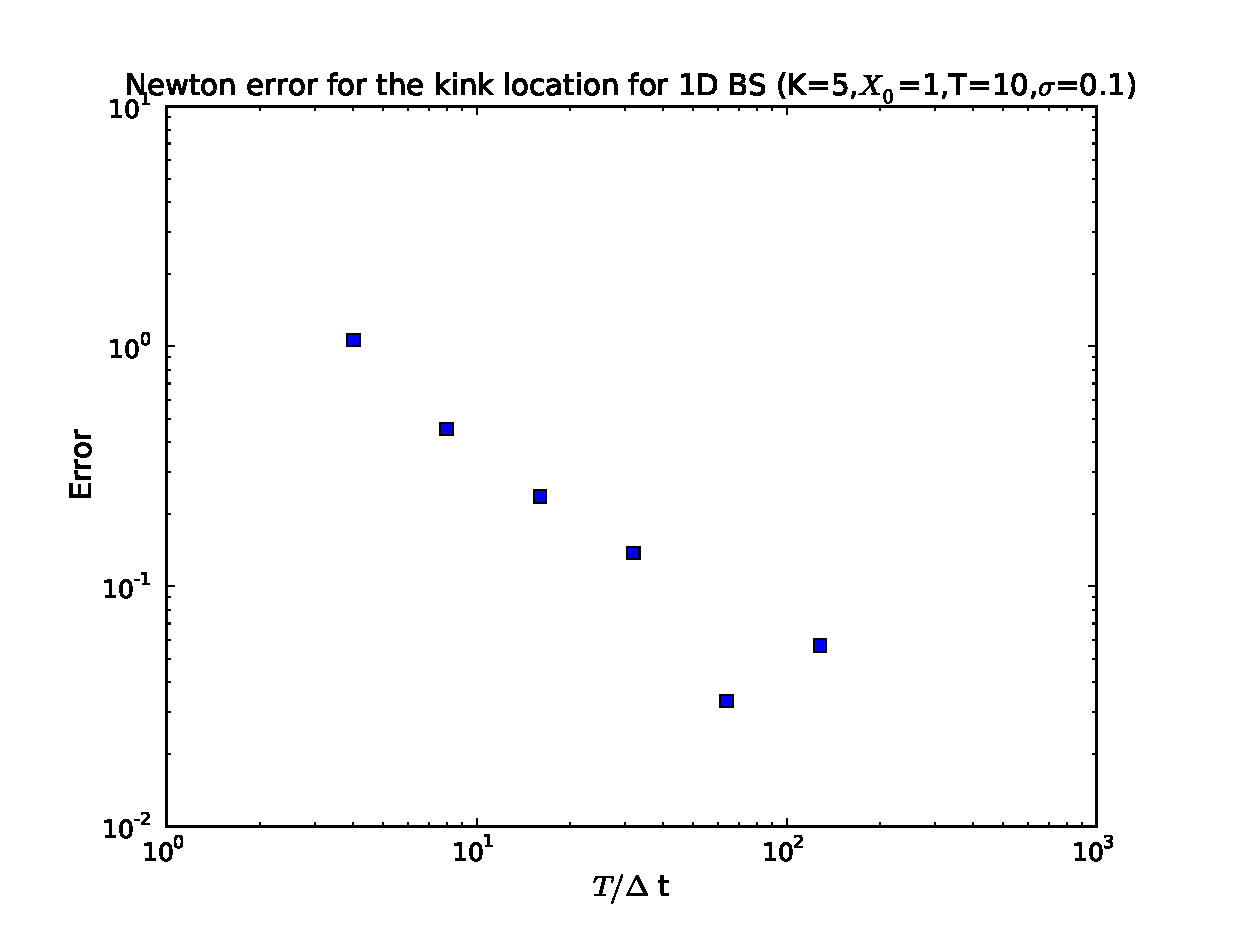
\includegraphics[scale=0.5]{./figures/kink_location_1D_BS_out_the_money.eps}
%\label{fig:1}
%\end{center}
%\end{figure}
%
%\begin{figure}[!h]
%	\begin{center}
%		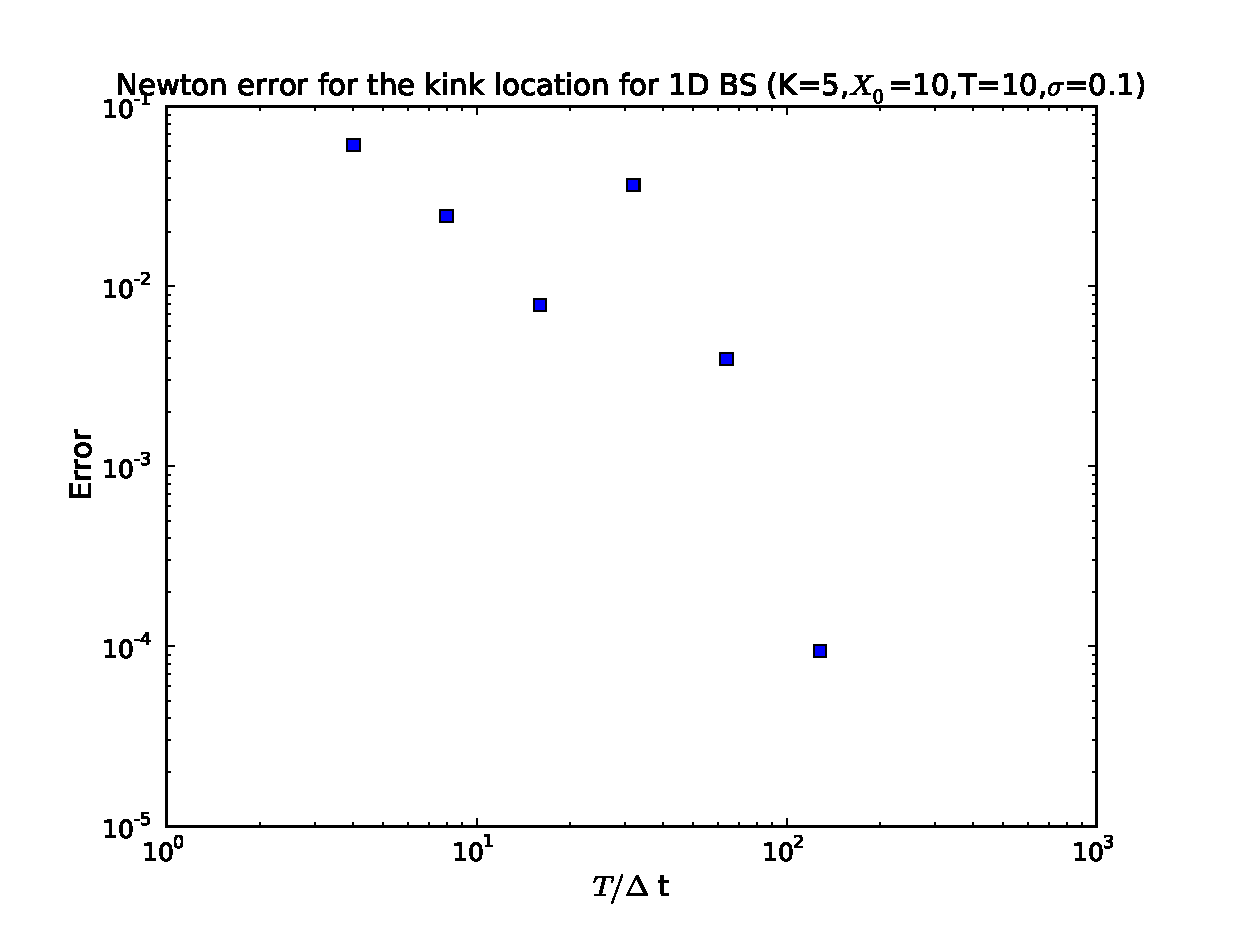
\includegraphics[scale=0.5]{./figures/kink_location_1D_BS_in_the_money.eps}
%		\label{fig:2}
%	\end{center}
%\end{figure}
%
%
%\begin{figure}[!h]
%	\begin{center}
%		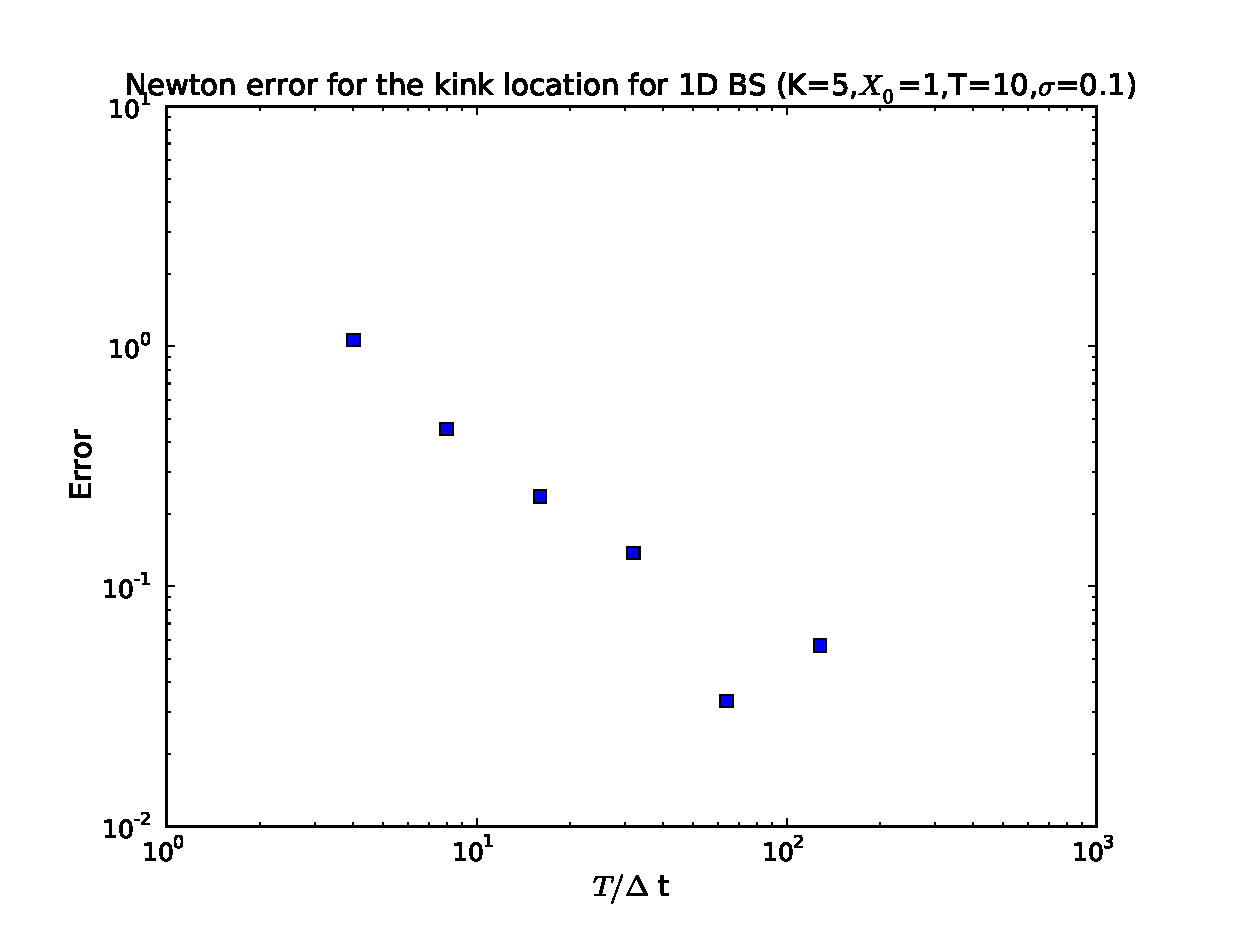
\includegraphics[scale=0.5]{./figures/kink_location_1D_BS_out_the_money.eps}
%		\label{fig:3}
%	\end{center}
%\end{figure}
%
%
%
%
%\newpage
%
%







%\begin{figure}[!h]
%	\centering
%	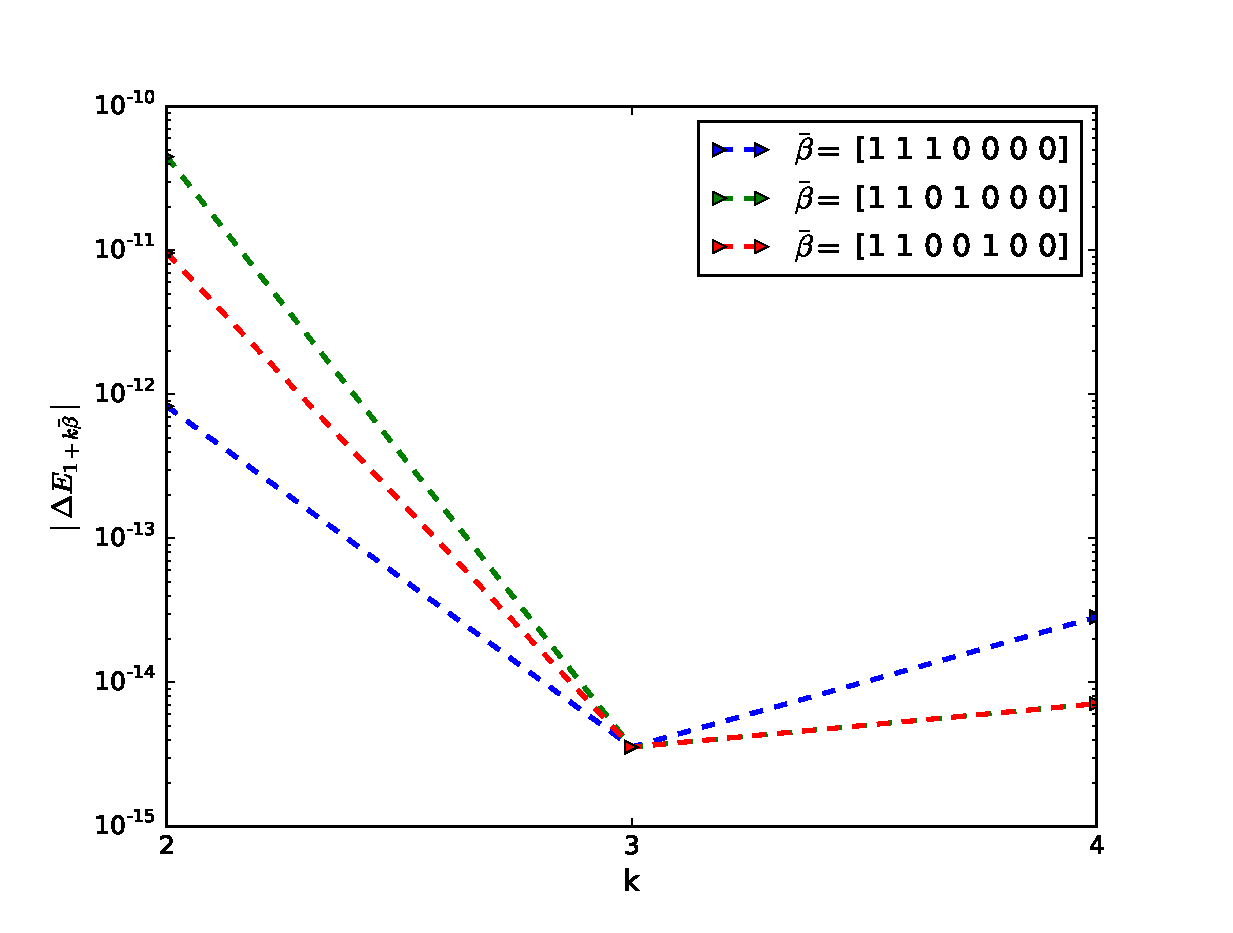
\includegraphics[width=0.6\linewidth]{./figures/mixed_difference_order3_1D_BS_N_8.eps}
%	
%	\caption{The rate of convergence of  third order mixed differences of  $\abs{\Delta E_{\beta}}$ ($\beta=\mathbf{1}+k \bar{\beta}$)): for  $N=8$.}
%	\label{fig:test6}
%\end{figure}





\subsection{The  basket call option under the discretized multi-dimensional Black-Scholes}\label{sec:The basket option under time stepping framework}

In the following, I present two ways of solving the root finding problem in multi-dimension. The first way, presented in Section \ref{sec: First way},  is an extension of Section \ref{sec:The discretized 1D Black-Scholes}, and the numerical results in Section \ref{sec:Result for the  $2$-dimensional Basket call option} are based on applying this way of numerical smoothing. In the second way, presented in Section \ref{sec: Second way}, we tried a different approach that is inspired by  the work of \cite{bayersmoothing}. However, the way I did it, it seems to me that we do not  need numerical smoothing and the smoothing can be done analytically.

\subsubsection{First way}\label{sec: First way}
In this suggested way, I try to extend the way we solved the one dimensional problem, as in Section \ref{sec:The discretized 1D Black-Scholes}, to higher dimensions.

We consider the basket option under multi-dimensional BS model where the process $\mathbf{X}$ is the discretized $d$-dimensional Black-Scholes model and the payoff function $g$ is given by
\begin{align}
	g(\mathbf{X}(T))=\max\left(\sum_{i=1}^{d} \omega_{i} X^{(i)}(T)-K,0  \right)	
\end{align}
Precisely, we are interested in the  $d$-dimensional lognormal example where the dynamics of the stock are given by

\begin{align}\label{lognormal_dynamics_basket}
	dX^{(i)}_t=\sigma^{(i)} X^{(i)}_t dB^{(i)}_t,
\end{align}

where $\{B^{(1)}, \dots,B^{(d)}\}$ are correlated Brownian motions with correlations $\rho_{ij}$.


In the discrete case, the numerical approximation of $X^{(j)}(T)$ satisfies


\begin{align}
	\bar{X}^{(j)}_T&=\Phi(\Delta t, z_1^{(j)}, \Delta B^{(j)}_0,\dots,\Delta B^{(j)}_{N-1}),  \quad 1 \le j \le d, \\ \nonumber
	&=\Phi(\Delta t, \Psi(z_1^{(j)},\dots,z_N^{(j)})), \quad 1 \le j \le d,
\end{align}
for some path function $\Phi$ and Brownian bridge map $\Psi$ as described in Section \ref{sec:Brwonian bridge construction}.

Using results from section \ref{sec:The discretized 1D Black-Scholes}, we have

\begin{align}
	\bar{X}^{(j)}(T)=X_0^{(j)} \prod_{i=0}^{N-1} \left[ 1+\frac{\sigma^{(j)}}{\sqrt{T}} z^{(j)}_1 \Delta t+ \sigma^{(j)} \Delta B^{(j)}_{i}\right], \quad 1 \le j \le d.
\end{align}
Therefore, in order to determine $\mathbf{y}_{\ast}=(y_{\ast}^{(1)},\dots,y_{\ast}^{(d)})$, we need to solve
\begin{align}
	\mathbf{x}=\sum_{j=1}^{d} \omega_j X^{(j)}_0 \prod_{i=0}^{N-1} \left[ 1+\frac{\sigma^{(j)}}{\sqrt{T}} y^{(j)}_{\ast}(\mathbf{x}) \Delta t+ \sigma^{(j)} \Delta B^{(j)}_{i}\right],
\end{align}

which implies that the location of the kink point for the approximate problem is equivalent to finding the roots of the polynomial $P(\mathbf{y}_\ast(K))$, given by
\begin{align}\label{polynomial_kink_location_basket}
	P(\mathbf{y}_{\ast}(K))&=\sum_{j=1}^{d} \omega_j X^{(j)}_0 \prod_{i=0}^{N-1} \left[ 1+\frac{\sigma^{(j)}}{\sqrt{T}} y^{(j)}_{\ast} \Delta t+ \sigma^{(j)} \Delta B^{(j)}_{i}\right]-K, \nonumber\\
	&=\sum_{j=1}^{d} \omega_j X^{(j)}_0 \left(\prod_{i=0}^{N-1} \left[ 1+\frac{\sigma^{(j)}}{\sqrt{T}} y_\ast^{(j)} \Delta t+ \sigma^{(j)} \Delta B^{(j)}_{i}\right]-\frac{K}{ \omega_j X^{(j)}_0  d}\right) \nonumber\\
	&=\sum_{j=1}^{d} \omega_j X^{(j)}_0 P^{(j)}\left(y_\ast^{(j)}\left(\frac{K}{ \omega_j X^{(j)}_0  d }\right)\right)
\end{align}

Therefore, the problem of finding the kink in the $d$-dimensional problem is brought to finding the location of the kink for each dimension by solving the root of the polynomial $P^{(j)}\left(y_\ast^{(j)}\left(\frac{K}{\omega_j X^{(j)}_0 }\right)\right)$.  

Using  \textbf{Newton iteration method}, we use the expression $P'=\frac{d P^{(j)}}{d y_\ast^{(j)}}$. If we denote $f_i^{(j)}(y)=1+\frac{\sigma^{(j)}}{\sqrt{T}} y \Delta t+ \sigma^{(j)} \Delta B^{(j)}_{i}$, then we can easily show that
\begin{align}\label{polynomial_kink_location_derivative_basket}
	P'^{(j)}(y)=\frac{\sigma^{(j)} \Delta t}{\sqrt{T}} \left( \prod_{i=0}^{N-1} f_i^{(j)}(y)\right) \left[ \sum_{i=0}^{N-1} \frac{1}{f_i^{(j)}(y)}\right].
\end{align}




Therefore, in this case, the integrand $h(\mathbf{z}^{(1)}_{-1},\dots,\mathbf{z}^{(d)}_{-1})$ (as expressed in \eqref{eq: pre_integration_step_wrt_y1_basket}) is given by

\begin{align}\label{smoothed_integrand_basket_opt_2d}
	h(\mathbf{z}^{(1)}_{-1},\dots,\mathbf{z}^{(d)}_{-1})&= \int_{\Omega}  \max  \left[ \left(\sum_{j=1}^{d} \Phi \circ \Psi(T;z_1^{(j)},\mathbf{z}^{(j)}_{-1})\right)-K,0\right]   \rho_d(z_1^{(1)},\dots,z_1^{(d)}) dz_1^{(1)}\dots dz_1^{(d)}.
\end{align}


We get the kink point by running Newton iteration in each dimension seperately for root solving of each polynomial $P^{(j)}$ as expressed in \eqref{polynomial_kink_location_basket} with a precision of $10^{-10}$. We  decompose the total integration domain $\Omega$  into sub-domains $\Omega_i,\: i=1,2,\dots, 2^d$ such that the integrand is smooth in the interior of  $\Omega_i$ and such that the kink is located along the boundary of these areas. The total integral is then given as the sum of the separate integrals, \ie
\begin{align}
	h(\mathbf{z}^{(1)}_{-1},\dots,\mathbf{z}^{(d)}_{-1}) &:=  \int_{\Omega}  \max  \left[ \left(\sum_{j=1}^{d} \Phi \circ \Psi(T;z_1^{(j)},\mathbf{z}^{(j)}_{-1})\right)-K,0\right]   \rho_d(z_1^{(1)},\dots,z_1^{(d)}) dz_1^{(1)}\dots dz_1^{(d)}  \nonumber\\
	&=\sum_{i=1}^{2^d}	\int_{\Omega_i} 
	\max  \left[ \left(\sum_{j=1}^{d} \Phi \circ \Psi(T;z_1^{(j)},\mathbf{z}^{(j)}_{-1})\right)-K,0\right]   \rho_d(z_1^{(1)},\dots,z_1^{(d)}) dz_1^{(1)}\dots dz_1^{(d)},
\end{align}

where we use Gauss-laguerre quadrature with $\beta$ points to get each part.

\FloatBarrier


\subsubsection{Second way}\label{sec: Second way}
 The $i$-th asset $X^{(i)}$ of the basket $(i=1,\dots,d)$ is given by 

\begin{equation}
X^{(i)}_{k \Delta t}=X^{(i)}_0 \exp\left( -\frac{\sigma_i^2}{2} k \Delta t +\sigma_i B^{(i)}_{k\Delta t}\right), \quad 1 \le k \le N  \COMMA
\end{equation} 
where $X^{(i)}_0$ is the current price of the $i$-th asset, $\sigma_i$ is the volatility of the $i$-th asset and $B=(B^{(1)},\dots, B^{(d)})$ is a $d$-dimensional Brownian motion. The correlation between $B^{(i)}$ and $B^{(j)}$ is denoted by $\rho_{ij}$. The payoff function of the European basket option is given by 
\begin{equation}\label{eq:basket_call_payoff}
f(Z)=\max\left(\sum_{i=1}^{d} c_i X^{(i)}_T(Z) -K,0\right)\COMMA
\end{equation}
where $c_i$ is the corresponding weight of the $i$-th asset, $Z \in \rset^{N \times d}$ is standard Gaussian  vector, and 


\begin{equation}
X^{(i)}_{k \Delta t} (Z)=X^{(i)}_0 e^{-\frac{\sigma_i^2}{2} k \Delta t} \exp\left(\sum_{j=1}^{d  N} C_{(k-1) d +i,j} Z_j\right) \PERIOD
\end{equation}
where $C$ is a $dN \times dN$-matrix with $C C^T=\bar{\Sigma}:=R  \otimes \Sigma$ ($\Sigma$ is $N \times N$ matrix  given by \eqref{eq:covariance_matrix_in_time}), and $R$ is an $d \times d$-matrix with $R_{ij}=\sqrt{T/N} \rho_{ij} \sigma_i\sigma_j$. 

Therefore, we have

\begin{align}\label{eq:asset_dynamics_last_inc}
X^{(i)}_{T} (Z)=X^{(i)}_{N \Delta t}(Z)&=X^{(i)}_0 e^{-\frac{\sigma_i^2}{2} T} \exp\left(\sum_{j=1}^{d  N} C_{(N-1) d +i,j} Z_j\right) \nonumber\\
&=\tilde{w}^{(i)}  \exp\left(A_{i\ast} Z\right)\nonumber\\
&=\tilde{w}^{(i)}  \exp\left(\widetilde{Z}^{(i)}\right)\COMMA
\end{align}
where $\tilde{w}^{(i)}=X^{(i)}_0 e^{-\frac{\sigma_i^2}{2} T} $,  $A$ is a   $d \times dN$  matrix such that $A:=\left(C_{(N-1) d +i,j} \right)_{1 \le i \le d, \: 1 \le j \le dN }$,  $A_{i\ast}$ is the $i$-th row vector of A, and $\widetilde{Z}=AZ$.

Let us denote by $\widetilde{\Sigma}$ the covariance matrix of $\widetilde{Z}$, then $\widetilde{\Sigma}=A A^T$. If we use the same approach in \cite{bayersmoothing}, Specifically Lemma $3.1$, then we can write 
\begin{equation}
\widetilde{\Sigma}=\widetilde{V} \widetilde{D} \widetilde{V}^T
\end{equation} 

such that $\tilde{D}=\text{diag}(\lambda_1^2, \dots, \lambda_d^2)$ is $d \times d$ diagonal matrix and $\widetilde{V} \in \rset^{d \times d}$ is an invertibe matrix, with the property that $\widetilde{V}_{i,1} \equiv 1,\: i=1,\dots,d$.


Going back to \eqref{eq:basket_call_payoff}, and replacing $\widetilde{Z}$ by $\widetilde{V} Y$, such that  $Y:=\widetilde{V}^{-1} \widetilde{Z} \sim \mathcal{N}(0,\widetilde{D})$, we obtain

\begin{align}\label{eq:basket_call_payoff_2}
f(Z)&=\max\left(\sum_{i=1}^{d} c_i X^{(i)}_T(Z) -K,0\right) \nonumber\\
&=\max\left(\sum_{i=1}^{d} w^{(i)} \exp\left(\widetilde{Z}^{(i)}\right) -K,0\right) \nonumber\\
&=\max\left(\sum_{i=1}^{d} w^{(i)} \exp\left((\widetilde{V} Y)^{(i)}\right) -K,0\right) \nonumber\\
&=\max\left(\sum_{i=1}^{d} w^{(i)} \exp\left( Y_1+ \sum_{j=2}^{d}\widetilde{V}_{ij} Y_j\right) -K,0\right) \nonumber\\
&=\max\left(h(Y_2, \dots,Y_d) e^{Y_1} -K,0\right) \COMMA
\end{align}

where $w^{(i)}=c_i \tilde{w}^{(i)}$ and $h(y_2,\dots,y_d):= \sum_{i=1}^{d} w^{(i)} \exp\left(\sum_{i=1}^{d} w^{(i)}  \sum_{j=2}^{d}\widetilde{V}_{ij} Y_j \right)$. 


Giving  \eqref{eq:basket_call_payoff_2}, and Lemma $3.3$ in \cite{bayersmoothing}, it seems to me that we do not  need numerical smoothing and the smoothing can be done analytically using conditional expectation formula. 







%For notation simplification, let us denote  by $\mathbf{Z}^{(i)}:=(Z_{N(i-1)+1}, \dots, Z_{iN})$ and  $\mathbf{Z}^{(i)}_{-1}:=(Z_{N(i-1)+2}, \dots, Z_{iN})$. 


%Going back to \eqref{eq:basket_call_payoff}, we have 
%\begin{align}\label{eq:basket_call_payoff_2}
%	f(Z)&=\max\left(\sum_{i=1}^{d} c_i S^{(i)}_T(Z) -K,0\right) \nonumber\\
%	&=\max\left(\sum_{i=1}^{d} w_i \exp\left(\sum_{j=1}^{dN}C_{(N-1) d +i,j} Z_j\right) -K,0\right) \nonumber\\
%	&=\max\left(\sum_{i=1}^{d} w_i \left( \exp\left(\sum_{\ell=1}^{d}C_{(N-1) d +i,(\ell-1)N+1} Z_{(\ell-1)N+1}+\sum_{\underset{j \neq (\ell-1)N+1, 1\le \ell\le d} {j=1}}^{dN}C_{(N-1) d +i,j} Z_j \right)\right) -K,0\right) \nonumber \\
%	&=\max\left(\sum_{i=1}^{d} w_i \exp(y_i)  \exp\left(\sum_{\underset{j \neq (\ell-1)N+1, 1\le \ell\le d} {j=1}}^{dN}C_{(N-1) d +i,j} Z_j \right) -K,0\right)\nonumber\\
%	&=\max\left(\sum_{i=1}^{d} w_i \exp(y_i)  h_i( \mathbf{Z}^{(1)}_{-1}, \dots \mathbf{Z}^{(d)}_{-1})-K,0\right)
%	\COMMA
%\end{align}
%where
%\begin{align*}
%	w_i&=c_i X^{(i)}_0 e^{-\frac{\sigma_i^2}{2} T}\\
%	y_i&=\sum_{\ell=1}^{d}C_{(N-1) d +i,(\ell-1)N+1} Z_{(\ell-1)N+1}\\
%	h_i( \mathbf{Z}^{(1)}_{-1}, \dots \mathbf{Z}^{(d)}_{-1})&=	\exp\left(\sum_{\underset{j \neq (\ell-1)N+1, 1\le \ell\le d} {j=1}}^{dN}C_{(N-1) d +i,j} Z_j \right)\PERIOD
%\end{align*}
%
%$y_i$ can be seen always as a linear combination including the first factors in each asset dimension.






\subsection{Summary of numerical results}
We conduct our experiments for $3$ different examples under discretized BS model: i) single binary, ii) single call, and  basket call options (We just includeded results for $2$-dimensional basket following the way suugested in Section \ref{sec: First way}, I still have issue for higher dimensions that we need to discuss, and this is maybe related to the way I am solving the problem in high dimension).

In Sections \ref{sec:Weak error plots_binary} ,\ref{sec:Weak error plots_call} and \ref{sec:Weak error plots_Basket_2D_call}, we estimate the weak error  (Bias) of MC combined with root finding, for the different  examples, for $2$ scenarios involving with/without  Richardson extrapolation. The conclusions of this section are: 
\begin{itemize}
	\item Without Richardson extrapolation: For all cases, we get a weak error of order $\Delta t$, with different  constants (See tables (\ref{Bias and Statistical errors of MC  for computing Binary option price  for different number of time steps, without Richardson extrapolation. The numbers between parentheses are the corresponding absolute errors.}, \ref{Bias and Statistical errors of MC  for computing Call option price  for different number of time steps, without Richardson extrapolation. The numbers between parentheses are the corresponding absolute errors.},\ref{Bias and Statistical errors of MC  for computing Basket 2d Call option price  for different number of time steps, without Richardson extrapolation. The numbers between parentheses are the corresponding absolute errors.}) for the corresponding bias values as well the statistical errors). 
	
	\item With Richardson extrapolation: For the case of binary  and $2$-dimensional basket call options, we get a weak error of order almost $\Delta t^2$. For the case of single call,   we get a weak error of order higher than $\Delta t^2$  (See tables (\ref{Bias and Statistical errors of MC  for computing Binary option price  for different number of time steps, with Richardson extrapolation (level $1$). The numbers between parentheses are the corresponding absolute errors.},\ref{Bias and Statistical errors of MC  for computing Call option price  for different number of time steps, with Richardson extrapolation (level $1$). The numbers between parentheses are the corresponding absolute errors.}) for the corresponding bias values as well the statistical errors).  
\end{itemize}


\begin{remark}
	We emphasize that the reported weak rates correspond to the pre-asymptotic regime that we are interested in. We are not interested on estimating the rates specifically but rather a sufficient precise estimate of the weak error (Bias), $\mathcal{E}_B(N)$, for different time steps $N$, in order to get the biased MC  solution for a given discretization, that we denoted $Q^N(\infty)$ in Section \ref{sec:Details of the MISC}.  For a fixed discretization, the corresponding biased solution will be set as a reference solution to the MISC method in order to estimate the quadrature error $\mathcal{E}_Q(TOL_{\text{MISC}},N)$.	
\end{remark}


In Sections \ref{sec:Comparing relative errors, binary}, \ref{sec:Comparing relative errors, call} and \ref{sec:Comparing relative errors, basket call}, we show tables and plots reporting  the different errors involved in MC method (bias and statistical error), and in MISC (Quadrature error). The quadrature error (see \eqref{eq:quadrature error}) is computed by subtracting the MISC solution from the biased solution, computed with sufficiently large  number of samples (to kill the statistical error). Given that both methods, MC and MISC, have the same bias,  the computational time of MC and MISC is compared such that the statistical error is almost equal to the stable quadrature error produced by MISC.

The conclusions of those sections are: 


\begin{itemize}
    
    \item For the case of single binary option (see Section \ref{sec:Results for the binary option example}), MISC coupled with Richardson extrapolation  is $3.5$ times faster than MC coupled with Richardson extrapolation, to achieve a total relative error around $0.3\%$ (See tables ( \ref{Total error of MISC and MC to compute Binary option price of the different tolerances for different number of time steps, with Richardson extrapolation (level $1$). The numbers between parentheses are the corresponding absolute errors.},\ref{Comparsion of the computational time of  MC and MISC, used to compute Binary option price  for different number of time steps, with Richardson extrapolation (level $1$)}) ).  Applying Richardson extrapolation brought a significant improvement for MISC (compare tables  ( \ref{Total error of MISC and MC to compute Binary option price of the different tolerances for different number of time steps, without Richardson extrapolation. The numbers between parentheses are the corresponding absolute errors.},\ref{Comparsion of the computational time of  MC and MISC, used to compute Binary option price  for different number of time steps, without Richardson extrapolation}) (no Richardson), tables ( \ref{Total error of MISC and MC to compute Binary option price of the different tolerances for different number of time steps, with Richardson extrapolation (level $1$). The numbers between parentheses are the corresponding absolute errors.},\ref{Comparsion of the computational time of  MC and MISC, used to compute Binary option price  for different number of time steps, with Richardson extrapolation (level $1$)})  (Richardson (level $1$)) and corresponding complexity plots).
	
	
	
	  \item For the case of single call option (see Section \ref{sec:Results for the call option example}), MISC  is $241$ times faster than MC, to achieve a total relative error below  $0.5\%$ (See tables ( \ref{Total error of MISC and MC to compute Call option price of the different tolerances for different number of time steps, without Richardson extrapolation. The numbers between parentheses are the corresponding absolute errors.},\ref{Comparsion of the computational time of  MC and MISC, used to compute Call option price  for different number of time steps, without Richardson extrapolation}) ).  Applying Richardson extrapolation brought a significant improvement for MISC (compare tables  ( \ref{Total error of MISC and MC to compute Call option price of the different tolerances for different number of time steps, without Richardson extrapolation. The numbers between parentheses are the corresponding absolute errors.},\ref{Comparsion of the computational time of  MC and MISC, used to compute Call option price  for different number of time steps, without Richardson extrapolation}) (no Richardson), tables ( \ref{Total error of MISC and MC to compute Call option price of the different tolerances for different number of time steps, with Richardson extrapolation (level $1$). The numbers between parentheses are the corresponding absolute errors.},\ref{Comparsion of the computational time of  MC and MISC, used to compute Call option price  for different number of time steps, with Richardson extrapolation (level $1$)})  (Richardson (level $1$)) and corresponding complexity plots).
	  
	\item For the case of $2$-dimensional basket call option (see Section \ref{sec:Result for the  $2$-dimensional Basket call option}), MISC  is $80$ times faster than MC, to achieve a total relative error around  $0.8\%$ (See tables ( \ref{Total error of MISC and MC to compute Basket 2dCall option price of the different tolerances for different number of time steps, without Richardson extrapolation. The numbers between parentheses are the corresponding absolute errors,beta_16},\ref{Comparsion of the computational time of  MC and MISC, used to compute Basket 2d Call option price  for different number of time steps, without Richardson extrapolation, beta_16}) ).

\end{itemize}

\subsection{Results for the single binary option example}\label{sec:Results for the binary option example}

In this case, the integrand $h(\mathbf{z}_{-1})$ is given by

\begin{align}\label{smoothed_integrand_binary_opt_2}
	h(\mathbf{z}_{-1})&= \int \mathbf{1}_{\Phi \circ \Psi(T;z_1,\mathbf{z}_{-1})>K}\frac{1}{\sqrt{2 \pi}} \operatorname{exp} (-z_1^2/2) dy \nonumber\\
	&=  P(Y>y_{\ast}(K)) ,
\end{align}
 
where  $y_{\ast}(x)$, is an invertible function that satisfies 
\begin{align}
	\Phi \circ \Psi (T;y_{\ast}(x),\mathbf{z}_{-1})=x	
\end{align}

We get the kink point by running Newton iteration with a precision of $10^{-10}$.

The paramters that we used in our numerical experiments are: $T=1$, $\sigma=0.4$ and $S_0=K=100$. The exact value of this case is $0.42074029$.

\subsubsection{Weak error plots} \label{sec:Weak error plots_binary}
In this section, we include the results of weak error rates, for the binary option example, for $2$ scenarios, without/with Richardson extrapolation (level $1$). We note that the weak errors plotted here correspond to relative errors.  The upper and lower bounds are $95\%$ confidence interval.

From figure \ref{fig:Weak_rate_binary}, we see that we get a weak error of order $\Delta t$ for the case without Richardson and we observe an improvement in the rate and the constant when using level $1$ of Richardson extrapolation. The corresponding values of the Bias are reported in tables (\ref{Bias and Statistical errors of MC  for computing Binary option price  for different number of time steps, without Richardson extrapolation. The numbers between parentheses are the corresponding absolute errors.},\ref{Bias and Statistical errors of MC  for computing Binary option price  for different number of time steps, with Richardson extrapolation (level $1$). The numbers between parentheses are the corresponding absolute errors.}).


\begin{figure}[h!]
	\centering
	\begin{subfigure}{.35\textwidth}
		\centering
		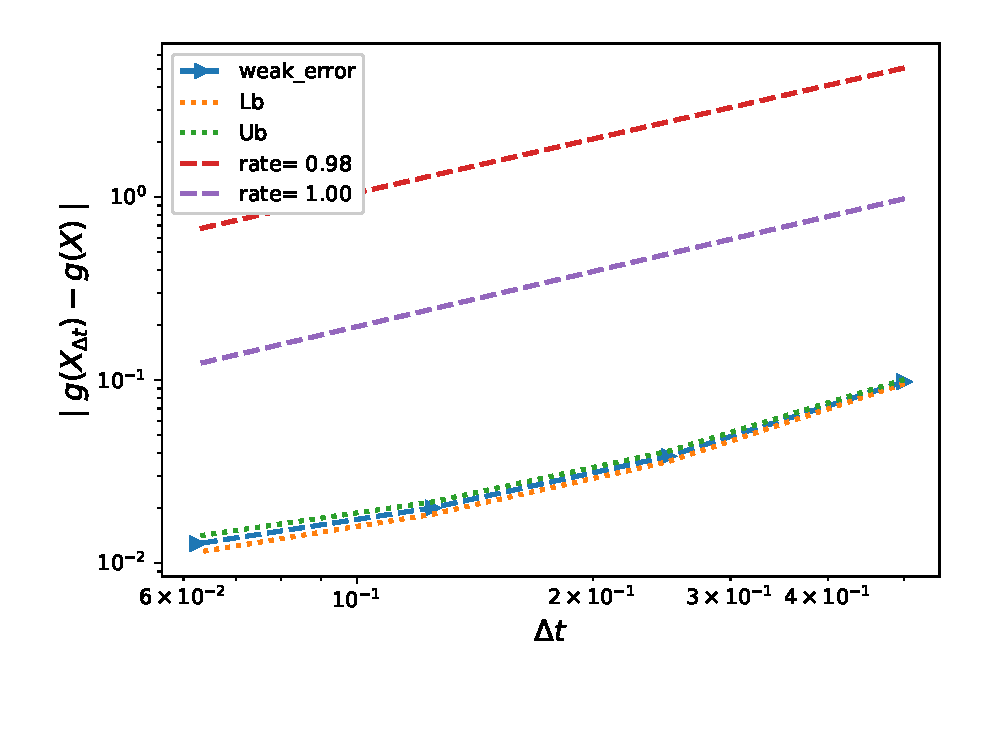
\includegraphics[width=1\linewidth]{./figures/binary_weak_error/without_richardson/weak_convergence_order_binary_option_relative_M_10_4}
		\caption{}
		\label{fig:sub3}
	\end{subfigure}%
	\begin{subfigure}{.35\textwidth}
		\centering
		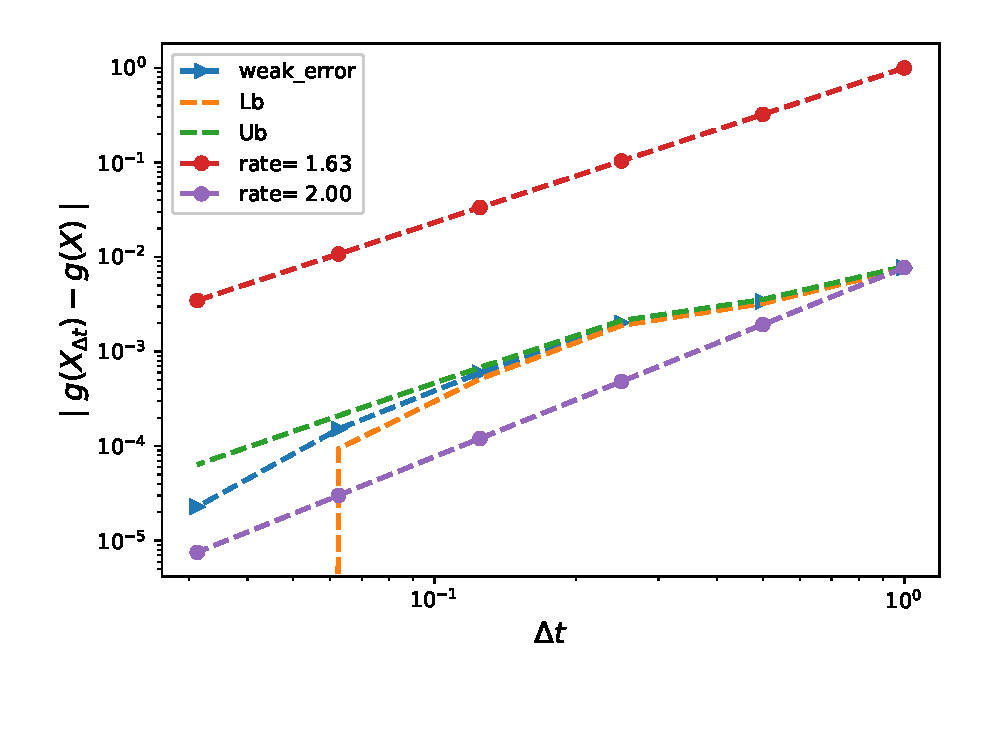
\includegraphics[width=1\linewidth]{./figures/binary_weak_error/with_richardson/weak_convergence_order_binary_richardson_relative_M_5_10_6}
		\caption{}
		\label{fig:sub4}
	\end{subfigure}
	
	\caption{The rate of convergence of the weak error for the binary option. a) $\abs{\expt{g(X_{\Delta t})}-g(X)}$  b)$\abs{\expt{2 g(X_{\Delta t/2}) -g(X_{\Delta t})}-g(X)}$.  }
	\label{fig:Weak_rate_binary}
\end{figure}




%\begin{figure}[h!]
%	\centering
%	\begin{subfigure}{.4\textwidth}
%		\centering
%		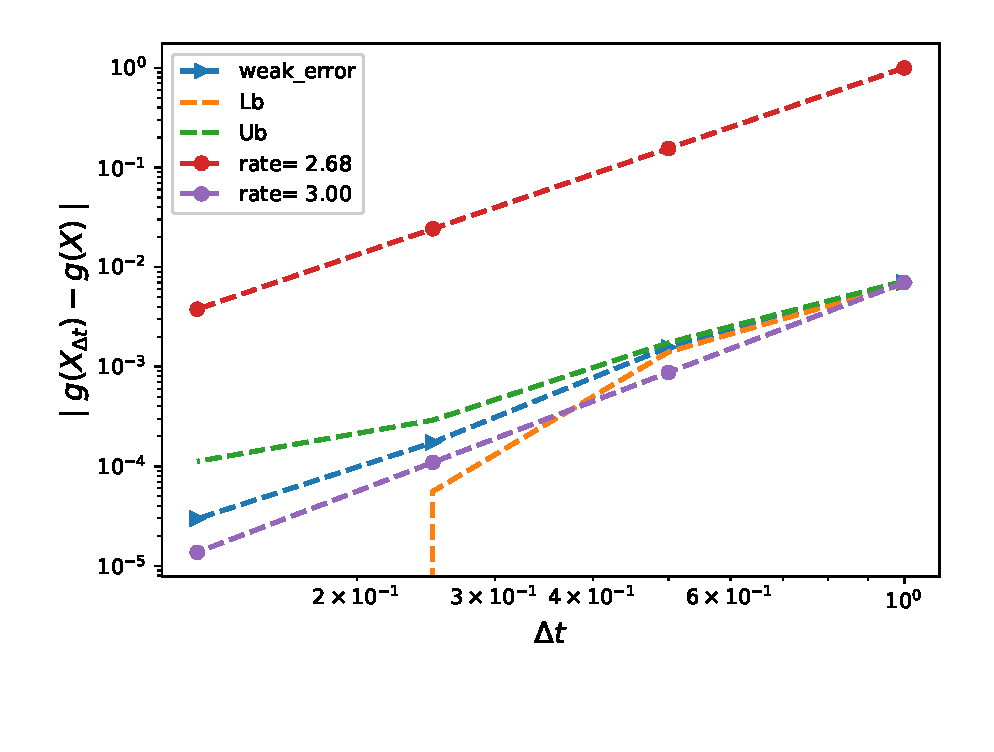
\includegraphics[width=1\linewidth]{./figures/binary_weak_error/with_richardson/weak_convergence_order_binary_richardson_level2_relative_M_5_10_6}
%		\caption{}
%		\label{fig:sub3}
%	\end{subfigure}%
%	\begin{subfigure}{.4\textwidth}
%		\centering
%		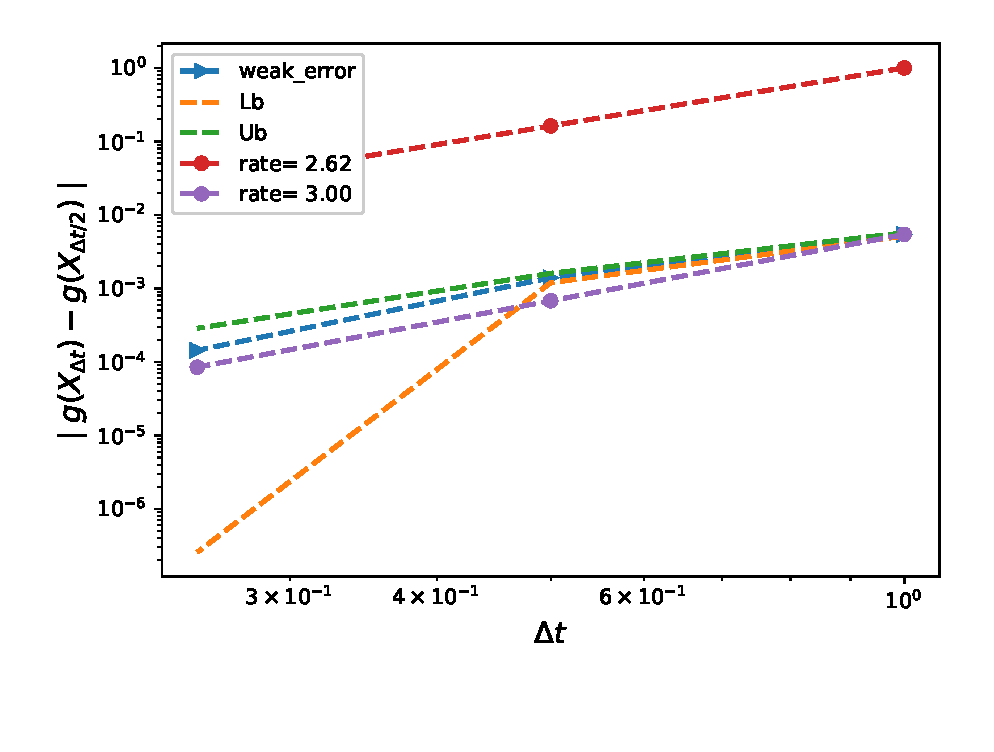
\includegraphics[width=1\linewidth]{./figures/binary_weak_error/with_richardson/weak_convergence_order_differences_binary_richardson_level2_relative_M_5_10_6}
%		\caption{}
%		\label{fig:sub4}
%	\end{subfigure}
%	
%	\caption{The rate of convergence of the weak error for the binary option, with Richardson extraploation (level $2$), using MC with $M=5.10^6$: a) $\abs{\frac{1}{3}\expt{8 g(X_{\Delta t/4}) -6g(X_{\Delta t/2}) +g(X_{\Delta t})}-g(X)}$  b) $\abs{\frac{1}{3}\expt{-8 g(X_{\Delta t/8}) +14g(X_{\Delta t/4})-7 (X_{\Delta t/2}) +g(X_{\Delta t})}}$ }
%	\label{fig:fig:Weak_rate_binary_with_rich_level2}
%\end{figure}
\FloatBarrier
\subsubsection{Comparing relative errors}\label{sec:Comparing relative errors, binary}


\subsubsection*{Without Richardson extrapolation}



\FloatBarrier
\begin{table}[h!]
	\centering
	\begin{tabular}{l*{6}{c}r}
		Method \textbackslash  Steps            & $2$ & $4$ & $8$ & $16$ &   \\
		\hline
		MISC ($TOL_{\text{MISC}}=5.10^{-1}$)  & $0.4620$ & $0.4404$ & $0.4299$ & $0.4250$  \\
		MISC ($TOL_{\text{MISC}}=10^{-1}$)  & $0.4620$ & $0.4404$ & $0.4301$ & $0.4250$  \\
		MISC ($TOL_{\text{MISC}}=5.10^{-2}$)  & $0.4620$ & $0.4403$ & $0.4300$ & $0.4250$  \\
		MISC ($TOL_{\text{MISC}}=10^{-2}$)  & $0.4620$ & $0.4406$ &  $0.4300$ & $0.4250$  \\
		MISC ($TOL_{\text{MISC}}=10^{-3}$)  & $0.4620$ & $0.4406$ & $0.4301$  & $0.4254$  \\
%		MISC ($TOL_{\text{MISC}}=10^{-4}$)  & $0.4620$ & $0.4406$ &  $0.4301$ & $-$  \\
		\hline
	%	MC method ($M=10^{5}$)   & $-$ & $-$  & $-$ & $-$ \\		
		MC method ($M=10^{4}$)   & $  0.4620$ & $    0.4369
		$  & $      0.4292$ & $  
		0.4261$ \\	
		\hline
	\end{tabular}
	\caption{Binary option price of the different methods for different number of time steps, without Richardson extrapolation.}
	\label{table: Binary option price of the different methods for different number of time steps, without Richardson extrapolation.}
\end{table}
\FloatBarrier
\begin{table}[h!]
	\centering
	\begin{tabular}{l*{6}{c}r}
		Method \textbackslash  Steps            & $2$ & $4$ & $8$ & $16$  \\
		\hline
		MC Bias $(M=10^{4})$  & 	$ \underset{(    
			0.0412)}{\mathbf{0.0980}}$  & $\underset{( 0.0162)}{\mathbf{ 0.0384
		}}$  & $\underset{(    0.0085
	)}{\mathbf{0.0201}}$ & $\underset{(   0.0053)}{\mathbf{   0.0127}}$\\ 
		
		MC Statistical error $(M=10^{4})$  &  $\underset{( 5.0e-04)} {\mathbf{1.2e-03}}$  & $\underset{( 5.0e-04)} {\mathbf{1.2e-03}}$ & $\underset{(3.4e-04)} {\mathbf{8.0e-04}}$ & $\underset{( 2.7e-04)} {\mathbf{6.5e-04}}$	\\
%			MC: Statistical error ($M=10^6$)  &  $\underset{( 5.0e-04)} {\mathbf{1.2e-03}}$  & $\underset{( 5.0e-04)} {\mathbf{1.2e-03}}$ & $\underset{( 5.0e-04)} {\mathbf{1.2e-03}}$ & $\underset{( 5.0e-04)} {\mathbf{1.2e-03}}$	\\
		\hline
	\end{tabular}
	\caption{Bias and statistical errors of MC  for computing binary option price  for different number of time steps, without Richardson extrapolation. The numbers between parentheses are the corresponding absolute errors.}
	\label{Bias and Statistical errors of MC  for computing Binary option price  for different number of time steps, without Richardson extrapolation. The numbers between parentheses are the corresponding absolute errors.}
\end{table}

\FloatBarrier




\begin{table}[h!]
	\centering
	\begin{tabular}{l*{6}{c}r}
		Method \textbackslash  Steps            & $2$ & $4$ & $8$ & $16$  \\
		\hline
		MISC ($TOL_{\text{MISC}}=5.10^{-1}$)  & $\underset{(2.4e-05)}{\mathbf{\red{1.0e-05}}}$ & $\underset{(0.0035)}{\mathbf{0.0083}}$  & $\underset{(0.0007)}{\mathbf{ 0.0017}}$ &$\underset{(0.0011)}{\mathbf{0.0026}}$ \\
		MISC ($TOL_{\text{MISC}}=10^{-1}$)   & $\underset{(2.4e-05)}{\mathbf{1.0e-05}}$ & $\underset{(0.0035)}{\mathbf{0.0083}}$ & $\underset{(0.0009)}{\mathbf{\red{0.0021}}}$ & $\underset{(0.0011)}{\mathbf{
				0.0026}}$ \\
		MISC ($TOL_{\text{MISC}}=5.10^{-2}$)  & $\underset{(2.4e-05)}{\mathbf{1.0e-05}}$& $\underset{(0.0034)}{\mathbf{0.0081}}$ & $\underset{(0.0008)}{\mathbf{ 0.0019}}$& $\underset{(0.0011)}{\mathbf{
				0.0026}}$ \\
		MISC ($TOL_{\text{MISC}}=10^{-2}$)  & $\underset{(2.4e-05)}{\mathbf{1.0e-05}}$ & $\underset{(0.0037)}{\mathbf{\red{0.0088}}}$ & $\underset{(0.0008)}{\mathbf{ 0.0019}}$ & $\underset{(0.0011)}{\mathbf{
				0.0026}}$ \\
		MISC ($TOL_{\text{MISC}}=10^{-3}$)  & $\underset{(2.4e-05)}{\mathbf{1.0e-05}}$ & $\underset{(0.0037)}{\mathbf{0.0088}}$& $\underset{(0.0009)}{\mathbf{0.0021}}$& $\underset{(0.0007)}{\mathbf{\red{ 0.0017}}}$ \\
%			MISC ($TOL_{\text{MISC}}=10^{-4}$)  & $\underset{(2.4e-05)}{\mathbf{1.0e-05}}$ & $\underset{(0.0037)}{\mathbf{0.0088}}$& $\underset{(0.0009)}{\mathbf{0.0021}}$& $\underset{(-)}{\mathbf{ -}}$ \\
		\hline
	\end{tabular}
	\caption{Quadrature error of MISC,  with different tolerances, to compute binary option price for different number of time steps, without Richardson extrapolation. The numbers between parentheses are the corresponding absolute errors. The values marked in red correspond to stable quadrature errors for MISC, and will be used for complexity comparison against MC.}
	\label{Quadrature error of MISC to compute Binary option price of the different tolerances for different number of time steps, without Richardson extrapolation. The numbers between parentheses are the corresponding absolute errors.}
\end{table}

\FloatBarrier
	\begin{figure}[h!]
	\centering
	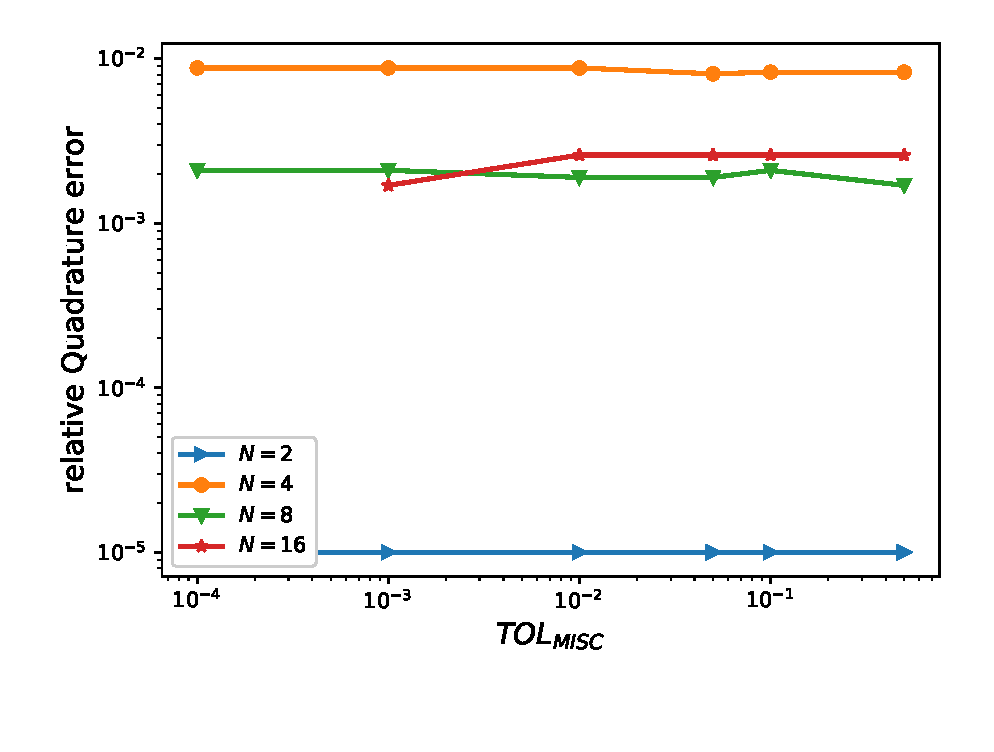
\includegraphics[width=0.4\linewidth]{./figures/Binary_MISC_quadrature_error/relative_quad_error_wrt_MISC_TOL_non_rich}
	
	
	\caption{Relative quadrature error of MISC, with different tolerances, to compute binary option price for different number of time steps, without Richardson extrapolation.}
	\label{fig:Quadrature_error_non_rich_binary}
\end{figure}



\FloatBarrier

\begin{table}[h!]
	\centering
	\begin{tabular}{l*{6}{c}r}
		Method \textbackslash  Steps         & $4$ & $8$ & $16$  \\
		\hline
		MISC ($TOL_{\text{MISC}}=5.10^{-1}$)   & $\mathbf{0.0467}$ & $\mathbf{ 0.0218}$ & $\mathbf{0.0153}$  \\
		MISC ($TOL_{\text{MISC}}=10^{-1}$) & $\mathbf{0.0467}$ & $\mathbf{\red{0.0222}}$ & $\mathbf{0.0153}$   \\
		MISC ($TOL_{\text{MISC}}=5.10^{-2}$)  & $\mathbf{0.0465}$ & $\mathbf{0.0220}$ & $\mathbf{0.0153}$  \\
		MISC ($TOL_{\text{MISC}}=10^{-2}$)  & $\mathbf{\red{ 0.0472}}$ & $\mathbf{ 0.0220}$ & $\mathbf{0.0153}$    \\
		MISC ($TOL_{\text{MISC}}=10^{-3}$)   & $\mathbf{ 0.0472}$  & $\mathbf{ 0.0222}$  & $\mathbf{\red{0.0144}}$\\
%	MISC ($TOL_{\text{MISC}}=10^{-4}$)  & $\mathbf{0.0980}$ & $\mathbf{0.0472}$ & $\mathbf{ 0.0222}$ & $\mathbf{-}$  \\
		\hline
		MC+root finding   &   $\mathbf{\red{0.0471 }}$ & $\mathbf{\red{0.0221}}$ & $\mathbf{\red{0.0141}}$  \\	
			MC     & $\mathbf{\red{0.0467}}$ & $\mathbf{\red{0.0222}}$ & $\mathbf{\red{0.0146}}$  \\	
		\hline
	
	\end{tabular}
	\caption{Total relative error of MISC, with different tolerances, and MC to compute binary option price for different number of time steps, without Richardson extrapolation.  The values marked in red, for MISC method, correspond to the total relative errors associated with  stable quadrature errors for MISC, and will be used for complexity comparison against MC.}
	\label{Total error of MISC and MC to compute Binary option price of the different tolerances for different number of time steps, without Richardson extrapolation. The numbers between parentheses are the corresponding absolute errors.}
\end{table}


\FloatBarrier

\begin{table}[h!]
	\centering
	\begin{tabular}{l*{6}{c}r}
		Method \textbackslash  Steps             & $4$ & $8$ & $16$ &   \\
		\hline
		MISC ($TOL_{\text{MISC}}=5.10^{-1}$)   & $0.8$ & $2$ & $9$  \\
		MISC ($TOL_{\text{MISC}}=10^{-1}$)   & $0.8$ & $\red{9}$ & $49$  \\
		MISC ($TOL_{\text{MISC}}=5.10^{-2}$)    & $1.3$ & $12$ & $59$  \\
		MISC ($TOL_{\text{MISC}}=10^{-2}$)   & $\red{2}$ & $14$ & $63$  \\
		MISC ($TOL_{\text{MISC}}=10^{-3}$)    & $2$ & $34$ & $\red{1090}$  \\
%    	MISC ($TOL_{\text{MISC}}=10^{-4}$)   & $0.3$ & $16$ & $193$ & $-$  \\
		\hline
		MC+root finding method    & $\red{9}$ & $\red{96}$ & $\red{141}$  \\
		MC method    & $\red{7}$ & $\red{95}$ & $\red{152}$  \\
		\hline
		Ratio of	$\text{(MC+root finding)}/\text{(MISC)}$  & $\red{4.5}$ & $\red{11}$ & $\red{0.13}$  \\
			Ratio of	$(\text{MC})/(\text{MISC})$ &  $\red{3.5}$ & $\red{11}$ & $\red{0.14}$  \\
			\hline
	\end{tabular}
	\caption{Comparison of the computational time of  MC and MISC, used to compute binary option price  for different number of time steps, without Richardson extrapolation. The average computational time of MC is computed over $10$ runs.}
	\label{Comparsion of the computational time of  MC and MISC, used to compute Binary option price  for different number of time steps, without Richardson extrapolation}
\end{table}



\FloatBarrier

	\begin{figure}[h!]
	\centering
	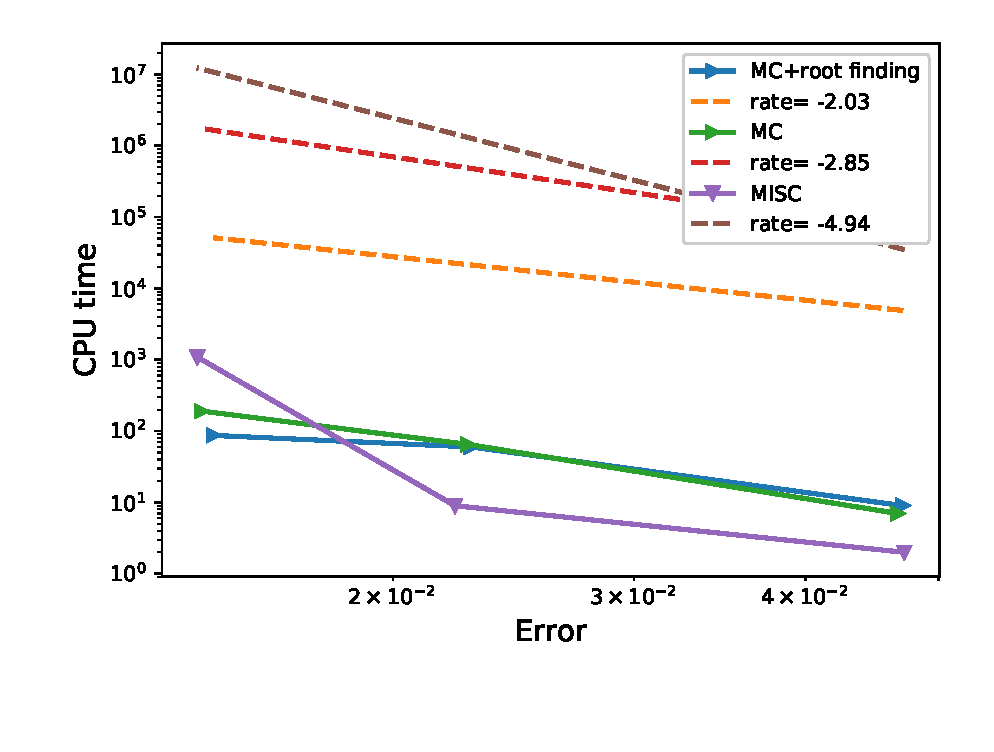
\includegraphics[width=0.4\linewidth]{./figures/Binary_Complexity_rates/error_vs_time}
	
	\caption{Complexity plot for MC and MISC for the case without Richardson extrapolation.}
	\label{fig:Complexity plot for MC and MISC , Binary, Non rich}
\end{figure}

\FloatBarrier

\subsubsection*{With Richardson extrapolation (level $1$)}


\FloatBarrier

\begin{table}[h!]
	\centering
	\begin{tabular}{l*{6}{c}r}
		Method \textbackslash  Steps            & $1-2$ & $2-4$ & $4-8$ & $8-16$ &   \\
		\hline
		MISC ($TOL_{\text{MISC}}=5.10^{-1}$)  & $0.4239$ & $0.4188$ & $0.4191$ & $0.4200$  \\
		MISC ($TOL_{\text{MISC}}=10^{-1}$)  &$0.4239$ & $0.4188$ &$0.4191$ & $0.4199$  \\
		MISC ($TOL_{\text{MISC}}=5.10^{-2}$) & $0.4239$ & $0.4188$ & $0.4190$ & $0.4199$  \\
		MISC ($TOL_{\text{MISC}}=10^{-2}$) &$0.4239$ & $0.4192$ & $0.4194$ & $0.4199$  \\
%		MISC ($TOL_{\text{MISC}}=10^{-3}$) & $0.4239$ & $0.4192$ & $0.4199$ & $0.4205$  \\
%			MISC ($TOL_{\text{MISC}}=10^{-4}$) & $0.4239$ & $0.4193$ & $0.4199$ & $-$  \\
		\hline
		MC method ($M=5.10^{6}$)   & $ 0.4240$ & $
		0.4224$ & $    0.4216$ & $  0.4210$  \\
		\hline
	\end{tabular}
	\caption{Binary option price of the different methods for different number of time steps, with Richardson extrapolation (level $1$).}
	\label{table: Binary option price of the different methods for different number of time steps, with Richardson extrapolation (level1).}
\end{table}

\FloatBarrier
\begin{table}[h!]
	\centering
	\begin{tabular}{l*{6}{c}r}
		Method \textbackslash  Steps            & $1-2$ & $2-4$ & $4-8$ & $8-16$  \\
		\hline
	MC Bias  ($M=5.10^{6}$)&$ \underset{(0.0032)}{\mathbf{0.0077}}$    & $\underset{(    0.0016
		)}{\mathbf{0.0039}}$  & $\underset{(0.0008)}{\mathbf{0.0020}}$  & $\underset{(0.0003)}{\mathbf{0.0006}}$\\
		MC Statistical error   ($M=5.10^{6}$)   & 	$ \underset{( 4.6e-05  )}{\mathbf{1.1e-04}}$  & $\underset{(3.5e-05)}{\mathbf{ 8.4e-05
	}}$  & $\underset{(2.5e-05)}{\mathbf{6.0e-05}}$ & $\underset{(   1.8e-05 )}{\mathbf{  4.2e-05 }}$\\ 
		
%		MC+root finding: Statistical error ($M=10^3$)     & 	$ \underset{( 3.5e-03  )}{\mathbf{8.3e-03}}$  & $\underset{(2.8e-03)}{\mathbf{ 6.6e-03
%		}}$  & $\underset{(1.8e-03)}{\mathbf{4.3e-03}}$ & $\underset{(  1.2e-03 )}{\mathbf{  2.9e-03 }}$\\ 
%		
		\hline
	\end{tabular}
	\caption{Bias and statistical errors of MC  for computing binary option price  for different number of time steps, with Richardson extrapolation (level $1$). The numbers between parentheses are the corresponding absolute errors.}
	\label{Bias and Statistical errors of MC  for computing Binary option price  for different number of time steps, with Richardson extrapolation (level $1$). The numbers between parentheses are the corresponding absolute errors.}
\end{table}

\FloatBarrier



\begin{table}[h!]
	\centering
	\begin{tabular}{l*{6}{c}r}
		Method \textbackslash  Steps            & $1-2$ & $2-4$ & $4-8$ & $8-16$  \\
		\hline
		MISC ($TOL_{\text{MISC}}=5.10^{-1}$)  & $\underset{(   1.0e-04)}{\mathbf{ \red{2.4e-04}}}$ & $\underset{(3.6e-03)}{\mathbf{8.6e-03}}$  & $\underset{(2.5e-03)}{\mathbf{5.9e-03}}$ &$\underset{(1.0e-03)}{\mathbf{2.4e-03}}$ \\
		MISC ($TOL_{\text{MISC}}=10^{-1}$)   & $\underset{(   1.0e-04)}{\mathbf{ 2.4e-04}}$ & $\underset{(3.6e-03)}{\mathbf{8.6e-03}}$  & $\underset{(2.5e-03)}{\mathbf{5.9e-03}}$ &$\underset{(   1.1e-04)}{\mathbf{ \red{2.6e-03}}}$ \\
		MISC ($TOL_{\text{MISC}}=5.10^{-2}$)  & $\underset{(   1.0e-04)}{\mathbf{ 2.4e-04}}$ & $\underset{(3.6e-03)}{\mathbf{8.6e-03}}$ & $\underset{(2.6e-03)}{\mathbf{6.2e-03}}$ &$\underset{(   1.1e-04)}{\mathbf{ 2.6e-03}}$ \\
		MISC ($TOL_{\text{MISC}}=10^{-2}$)  & $\underset{(   1.0e-04)}{\mathbf{ 2.4e-04}}$ & $\underset{(3.2e-03)}{\mathbf{\red{7.6e-03}}}$  & $\underset{(2.2e-03)}{\mathbf{\red{5.2e-03}}}$ &$\underset{(   1.1e-04)}{\mathbf{ 2.6e-03}}$\\
%		MISC ($TOL_{\text{MISC}}=10^{-3}$)  & $\underset{(   1.0e-04)}{\mathbf{ 2.4e-04}}$ & $\underset{(3.2e-03)}{\mathbf{7.6e-03}}$  & $\underset{(1.7e-03)}{\mathbf{4.0e-03}}$ &$\underset{(   5.e-04)}{\mathbf{1.2e-03}}$ \\
%	MISC ($TOL_{\text{MISC}}=10^{-4}$)  & $\underset{(   1.0e-04)}{\mathbf{ 2.4e-04}}$ & $\underset{(3.1e-03)}{\mathbf{7.4e-03}}$  & $\underset{(1.7e-03)}{\mathbf{4.0e-03}}$ &$\underset{()}{\mathbf{}}$ \\
		\hline
	\end{tabular}
	\caption{Quadrature error of MISC, with different tolerances,  to compute binary option price for different number of time steps, with Richardson extrapolation (level $1$). The numbers between parentheses are the corresponding absolute errors. The values marked in red correspond to stable quadrature errors for MISC, and will be used for complexity comparison against MC.}
	\label{Quadrature error of MISC to compute Binary option price of the different tolerances for different number of time steps, with Richardson extrapolation (level $1$). The numbers between parentheses are the corresponding absolute errors.}
\end{table}


\FloatBarrier
	\begin{figure}[h!]
	\centering
	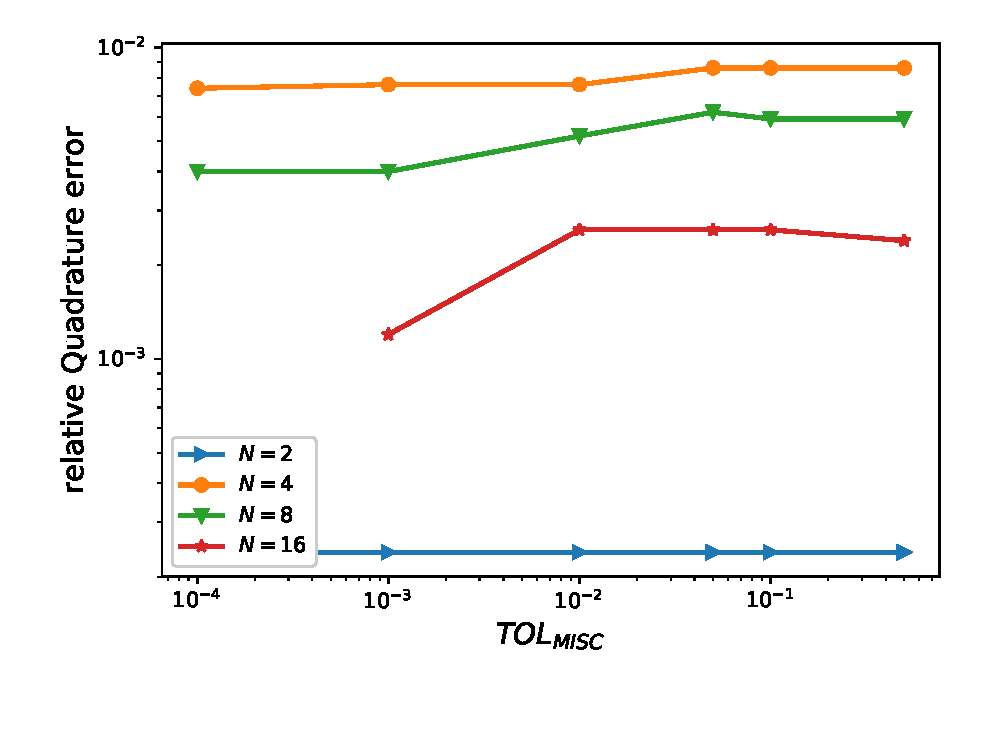
\includegraphics[width=0.4\linewidth]{./figures/Binary_MISC_quadrature_error/relative_quad_error_wrt_MISC_TOL_with_rich}
	
	
	\caption{Relative quadrature error of MISC, with different tolerances, to compute binary option price of the different tolerances for different number of time steps, with Richardson extrapolation.}
	\label{fig:Quadrature_error_with_rich_binary}
\end{figure}

\FloatBarrier

\begin{table}[h!]
	\centering
	\begin{tabular}{l*{6}{c}r}
		Method \textbackslash  Steps          & $2-4$ & $4-8$ & $8-16$  \\
		\hline
		MISC ($TOL_{\text{MISC}}=5.10^{-1}$)  & $\mathbf{0.0125}$ & $\mathbf{0.0079}$ & $\mathbf{0.0030}$  \\
		MISC ($TOL_{\text{MISC}}=10^{-1}$)  &    $\mathbf{0.0125}$ & $\mathbf{0.0079}$ & $\mathbf{\red{0.0032}}$  \\
		MISC ($TOL_{\text{MISC}}=5.10^{-2}$) & $\mathbf{0.0125}$ & $\mathbf{0.0082}$ & $\mathbf{0.0032}$  \\
		MISC ($TOL_{\text{MISC}}=10^{-2}$)   & $\mathbf{\red{0.0115}}$ & $\mathbf{\red{0.0072}}$ & $\mathbf{0.0032}$  \\
%		MISC ($TOL_{\text{MISC}}=10^{-3}$) &   $\mathbf{0.0079}$ & $\mathbf{0.0115}$ & $\mathbf{0.0060}$ & $\mathbf{0.0018}$  \\
%
%	MISC ($TOL_{\text{MISC}}=10^{-4}$) &   $\mathbf{0.0079}$ & $\mathbf{0.0113}$ & $\mathbf{0.0060}$ & $\mathbf{-}$  \\
		\hline
		MC+root finding   & $\mathbf{\red{0.0111}}$ & $\mathbf{\red{0.0070}}$ & $\mathbf{\red{0.0035}}$  \\	
			MC     & $\mathbf{\red{0.0116}}$ & $\mathbf{\red{0.0073}}$ & $\mathbf{\red{0.0029}}$  \\	
		\hline
		
	\end{tabular}
	\caption{Total relative error of MISC, with different tolerances, and MC to compute binary option price for different number of time steps, with Richardson extrapolation (level $1$).  The values marked in red, for MISC method, correspond to the total relative errors associated with  stable quadrature errors for MISC, and will be used for complexity comparison against MC.}
	\label{Total error of MISC and MC to compute Binary option price of the different tolerances for different number of time steps, with Richardson extrapolation (level $1$). The numbers between parentheses are the corresponding absolute errors.}
\end{table}



\FloatBarrier


\begin{table}[h!]
	\centering
	\begin{tabular}{l*{6}{c}r}
		Method \textbackslash  Steps         & $2-4$ & $4-8$ & $8-16$ &   \\
		\hline
		MISC ($TOL_{\text{MISC}}=5.10^{-1}$) & $1$ & $4$ & $9$  \\
		MISC ($TOL_{\text{MISC}}=10^{-1}$) & $1$ & $8$ & $\red{42}$  \\
		MISC ($TOL_{\text{MISC}}=5.10^{-2}$)  & $1$ & $10$ & $72$  \\
		MISC ($TOL_{\text{MISC}}=10^{-2}$)   & $\red{4}$ & $\red{15}$ & $78$  \\
%		MISC ($TOL_{\text{MISC}}=10^{-3}$)   &$0.3$ & $4$ & $100$ & $2253$  \\
%			MISC ($TOL_{\text{MISC}}=10^{-4}$)   &$0.3$ & $68$ & $392$ & $$  \\
		\hline
		MC+root finding method      & $\red{48}$ & $\red{62}$ & $\red{122 }$  \\
			MC    & $\red{12}$ & $\red{23}$ & $\red{147}$  \\
		\hline
			Ratio of	$\text{(MC+root finding)}/\text{(MISC)}$  & $\red{12}$ & $\red{4.1}$ & $\red{2.9}$  \\
		Ratio of	$(\text{MC})/(\text{MISC})$ & $\red{3}$ & $\red{1.5}$ & $\red{3.5}$  \\
		\hline
	\end{tabular}
	\caption{Comparison of the computational time of  MC and MISC, used to compute binary option price  for different number of time steps, with Richardson extrapolation (level $1$). The average computational time of MC is computed over $10$ runs.}
	\label{Comparsion of the computational time of  MC and MISC, used to compute Binary option price  for different number of time steps, with Richardson extrapolation (level $1$)}
\end{table}

\FloatBarrier
	\begin{figure}[h!]
\centering
\includegraphics[width=0.4\linewidth]{./figures/Binary_Complexity_rates/error_vs_time_rich}

\caption{Complexity plot for MC and MISC for the case with Richardson extrapolation.}
\label{fig:Complexity plot for MC and MISC , Binary, with rich}
\end{figure}






\FloatBarrier

\begin{figure}[h!]
\centering
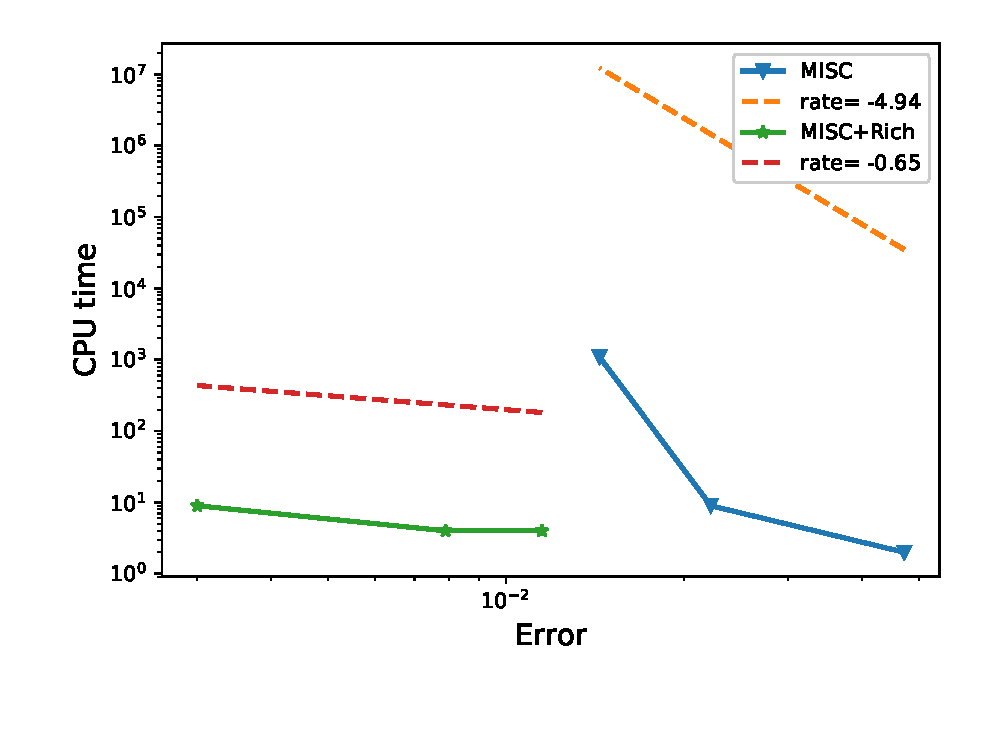
\includegraphics[width=0.4\linewidth]{./figures/Binary_Complexity_rates/error_vs_time_comparison}

\caption{Complexity plot for MISC without and with Richardson extrapolation, for the binary option.}
\label{fig:Complexity plot for MC and MISC , Binary, comparison}
\end{figure}

\FloatBarrier



%In the following, we compare the  relative errors for the binary option example under Black-Scholes model (see Tables (\ref{Relative error of the binary option price of the different tolerances for different number of time steps.}, \ref{Relative error of Call option price of the different tolerances for different number of time steps, using Richardson extrapolation (level $1$)})). We report the results for $2$ scenarios: i) Without using Richardson extrapolation, ii) Using level $1$ Richardson extrapoaltion.  You may see appendix \ref{appendix:Call prices for different methods_binary} for the values of binary option prices.
%
%Given the normalized bias computed by MC method (See Section \ref{sec:Weak error plots_binary}) (reported as bold values in the tables), we report in red in each table the smallest tolerance that MISC required to get below that relative bias (I do not put values for smaller tolerances, once the required bias is reached).
%
%From the tables (\ref{Relative error of the binary option price of the different tolerances for different number of time steps.}, \ref{Relative error of Call option price of the different tolerances for different number of time steps, using Richardson extrapolation (level $1$)})), we may observe that to get a relative error below $1\%$, we need around $16$ time steps for the case without Richardson extrapolation compared to only using $1$ time step in the coarse level for the case of level $1$ Richardson extraplation. 



%\begin{table}[h!]
%	\centering
%	\begin{tabular}{l*{5}{c}r}
%		Method \textbackslash  Steps    &$1-2$        & $2-4$ & $4-8$ & $8-16$  \\
%		\hline
%		MISC ($TOL_{\text{MISC}}=5.10^{-1}$)  &$\red{0.0076}$ & $0.0045$ & $0.0031$ & $0.0017$  \\
%		MISC ($TOL_{\text{MISC}}=10^{-2}$)  &$-$ & $\red{0.0036}$ & $0.0031$ & $0.0014$  \\
%		MISC ($TOL_{\text{MISC}}=10^{-3}$) & $-$ & $-$ & $  \red{0.0021}$ & $\red{0.0005}$   \\
%		MC method ($M=5.10^{6}$)&$ \mathbf{0.0077}$    & $\mathbf{0.0039}$  & $\mathbf{0.0020}$  & $\mathbf{0.0006}$ \\
%		\hline
%	\end{tabular}
%	\caption{Relative error of the binary option price of the different tolerances for different number of time steps, using Richardson extrapolation (level $1$)}
%	\label{Relative error of binary option price of the different tolerances for different number of time steps, using Richardson extrapolation (level $1$)}
%\end{table}


\FloatBarrier
\subsection{Results for the single call option example}\label{sec:Results for the call option example}


In this case, the integrand $h(\mathbf{z}_{-1})$ is given by

\begin{align}\label{smoothed_integrand_call_opt_2}
	h(\mathbf{z}_{-1})&= \int_{\Omega}  \max \left(\Phi \circ \Psi(T;z_1,\mathbf{z}_{-1})-K,0\right) \frac{1}{\sqrt{2 \pi}} \operatorname{exp}(-z_1^2/2) dz_1 
\end{align}


We get the kink point by running Newton iteration with a precision of $10^{-10}$. We  decompose the total integration domain $\Omega$  into sub-domains $\Omega_i,\: i=1,2$ such that the
integrand is smooth in the interior of 
$\Omega_i$ and such that the kink is located along the boundary of these areas. The total integral is then given
as the sum of the separate integrals, \ie
\begin{align}
	h(\mathbf{z}_{-1}) &:=  \int_{\Omega} \max \left(\Phi \circ \Psi(T;z_1,\mathbf{z}_{-1})-K,0\right) \frac{1}{\sqrt{2 \pi}} \operatorname{exp}(-z_1^2/2) dy \\ \nonumber
	&=\sum_{i=1}^{2}	\int_{\Omega_i} \max \left(\Phi \circ \Psi(T;z_1,\mathbf{z}_{-1})-K,0\right) \frac{1}{\sqrt{2 \pi}} \operatorname{exp}(-z_1^2/2) dz_1,
\end{align}


where we use Gauss-laguerre quadrature with $\beta$ points to get each part.

The paramters that we used in our numerical experiments are: $T=1$, $\sigma=0.4$ and $S_0=K=100$. The exact value of this case is $15.85193755$.











\subsubsection{Weak error plots} \label{sec:Weak error plots_call}



In this section, we include the results of weak error rates for  the call option for $2$ scenarios, without/with Richardson extrapolation (level $1$). We note that the weak errors plotted here correspond to relative errors.  The upper and lower bounds are $95\%$ confidence interval.

We can see from figure \ref{fig:Weak_rate_call_beta_32} that we get a weak error of order $\Delta t$ for the case without Richardson extrapolation and  an improvement in the rate and the constant when using level $1$ of Richardson extrapolation, approximately of order $\Delta t^2$.  



%\subsubsection*{$\beta=10$}
%From figure \ref{fig:Weak_rate_call_without_rich}, we see that we get a weak error of order $\Delta t$. From figure \ref{fig:fig:Weak_rate_call_with_rich}, we observe that we get a weak error of order $\Delta t^2$ (if eliminate the  last point having a wide confidence interval point). From figure \ref{fig:Weak_rate_call_with_rich_level2}, we observe that we get an almost constant weak error, with that constant being the smallest cpmpared to without and with level $1$ Ricardson extrapolation. The upper and lower bounds are $95\%$ confidence interval.

%\begin{figure}[h!]
%	\centering
%	\begin{subfigure}{.35\textwidth}
%		\centering
%		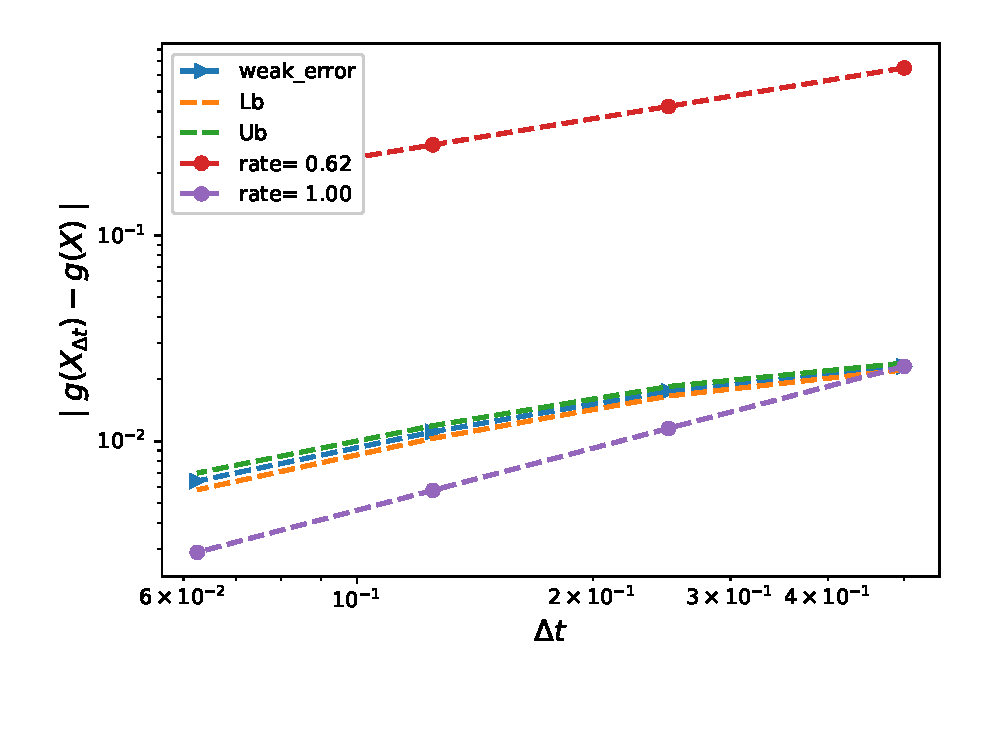
\includegraphics[width=1\linewidth]{./figures/weak_error_rates_call/Beta_10/without_richardson/weak_convergence_order_call_option_relative_M_10_5}
%		\caption{}
%		\label{fig:sub3}
%	\end{subfigure}%
%	\begin{subfigure}{.35\textwidth}
%		\centering
%		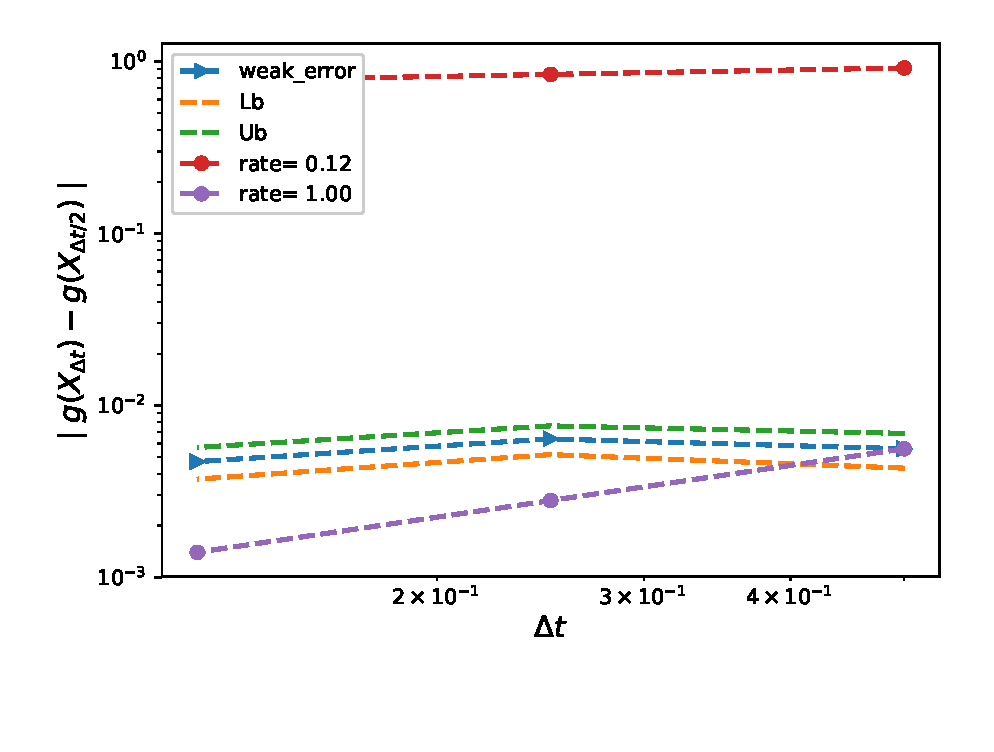
\includegraphics[width=1\linewidth]{./figures/weak_error_rates_call/Beta_10/without_richardson/weak_convergence_order_differences_call_option_relative_M_10_5}
%		\caption{}
%		\label{fig:sub4}
%	\end{subfigure}
%	
%	\caption{The rate of convergence of the weak error for the call option, without Richardson extraploation, using MC with $M=10^5$: a) $\abs{\expt{g(X_{\Delta t})}-g(X)}$  b) $\abs{\expt{g(X_{\Delta t})-g(X_{\Delta t/2})}}$ }
%	\label{fig:Weak_rate_call_without_rich}
%\end{figure}
%\begin{figure}[h!]
%	\centering
%	\begin{subfigure}{.35\textwidth}
%		\centering
%		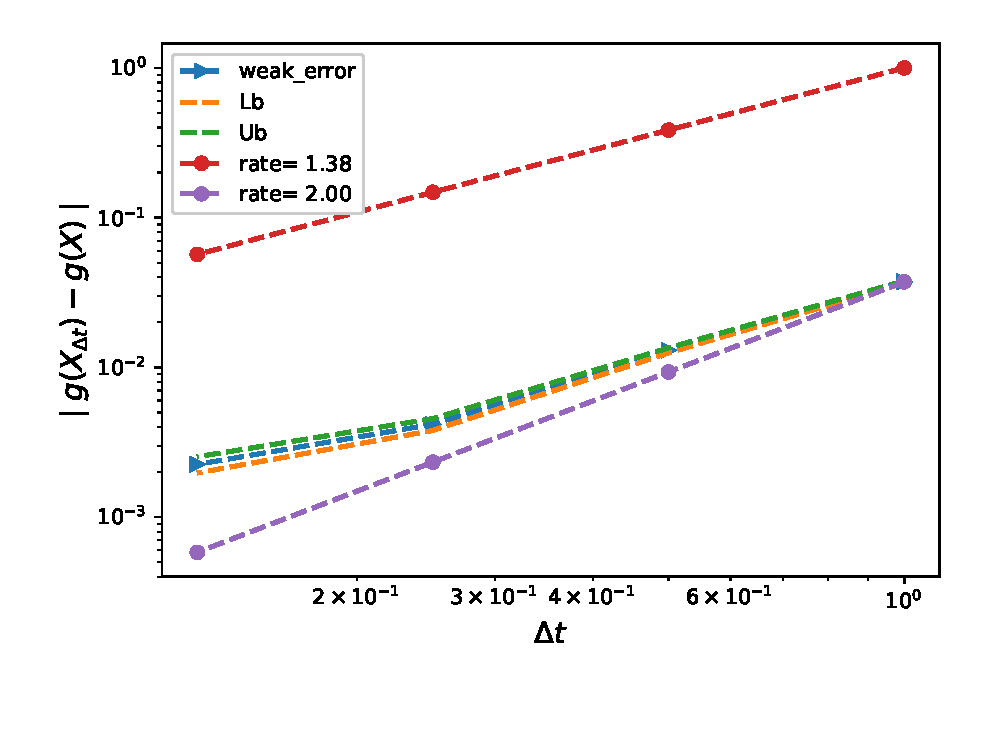
\includegraphics[width=1\linewidth]{./figures/weak_error_rates_call/Beta_10/with_richardson/weak_convergence_order_call_richardson_relative_M_10_6}
%		\caption{}
%		\label{fig:sub3}
%	\end{subfigure}%
%	\begin{subfigure}{.35\textwidth}
%		\centering
%		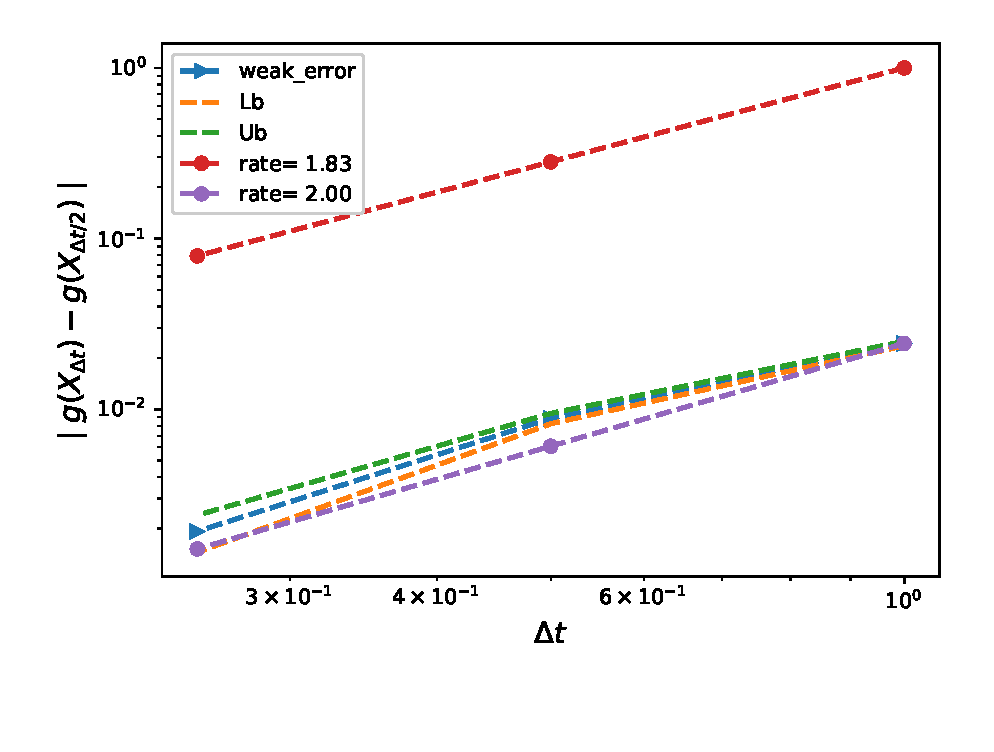
\includegraphics[width=1\linewidth]{./figures/weak_error_rates_call/Beta_10/with_richardson/weak_convergence_order_differences_call_richardson_relative_M_10_6}
%		\caption{}
%		\label{fig:sub4}
%	\end{subfigure}
%	
%	\caption{The rate of convergence of the weak error for the  call option with Richardson extraploation, using MC with $M=10^6$: a) $\abs{\expt{2 g(X_{\Delta t/2}) -g(X_{\Delta t})}-g(X)}$  b) $\abs{\expt{3 g(X_{\Delta t/2})-g(X_{\Delta t})-2 g(X_{\Delta t/4})}}$ }
%	\label{fig:fig:Weak_rate_call_with_rich}
%\end{figure}



%\begin{figure}[h!]
%	\centering
%	\begin{subfigure}{.4\textwidth}
%		\centering
%		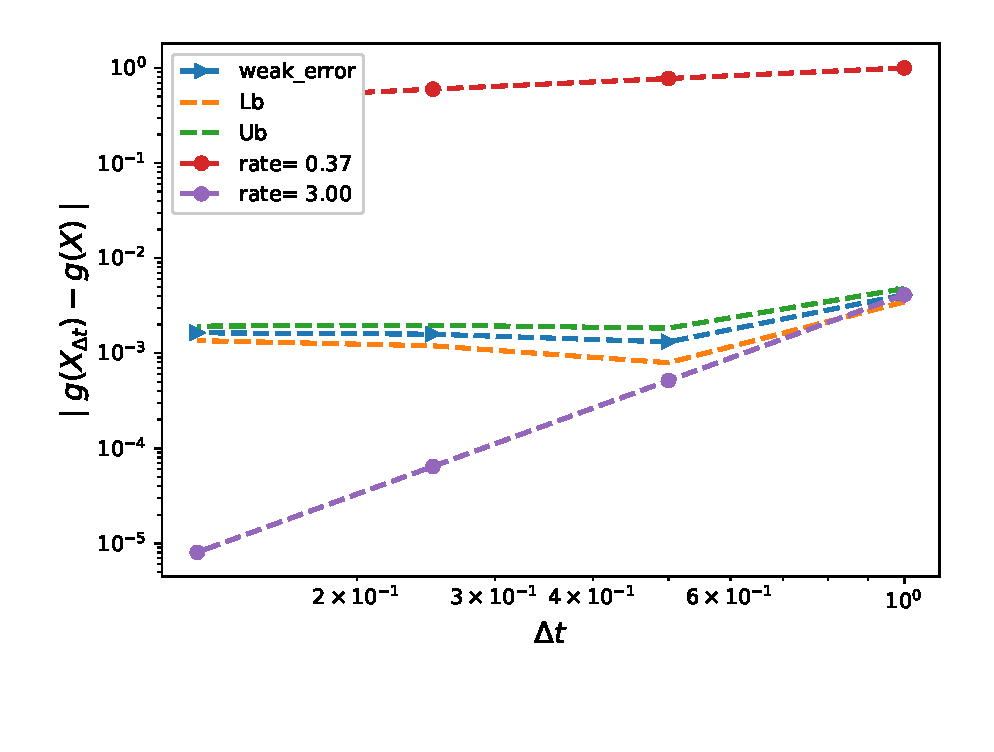
\includegraphics[width=1\linewidth]{./figures/weak_error_rates_call/Beta_10/with_richardson/weak_convergence_order_Call_richardson_level2_relative_M_10_6}
%		\caption{}
%		\label{fig:sub3}
%	\end{subfigure}%
%	\begin{subfigure}{.4\textwidth}
%		\centering
%		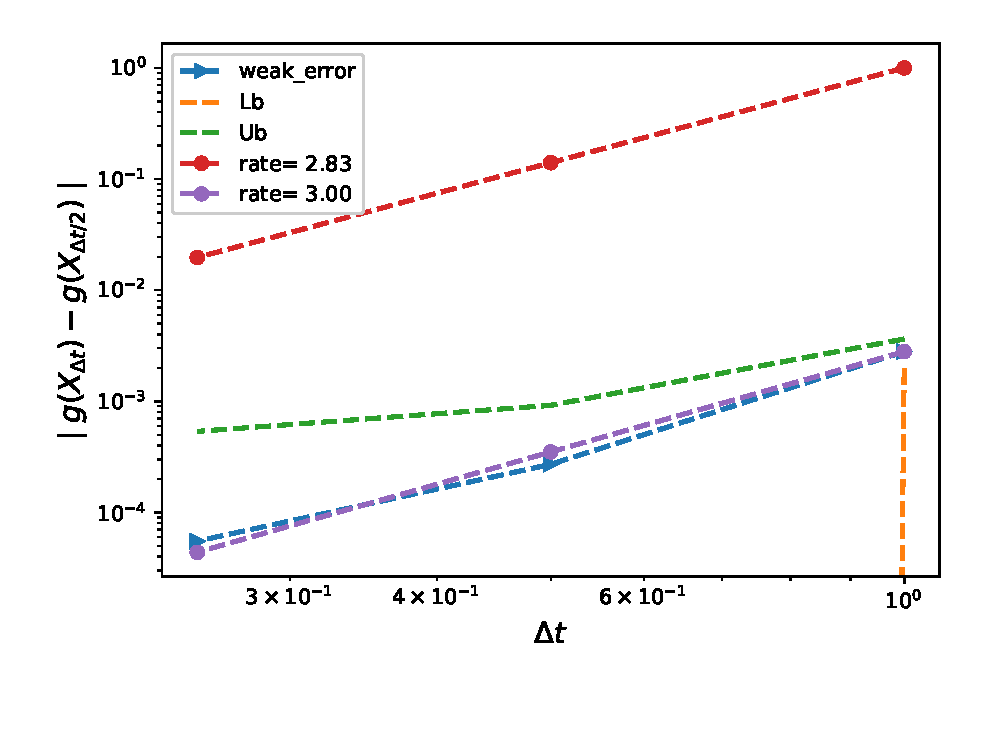
\includegraphics[width=1\linewidth]{./figures/weak_error_rates_call/Beta_10/with_richardson/weak_convergence_order_differences_Call_richardson_level2_relative_M_10_6}
%		\caption{}
%		\label{fig:sub4}
%	\end{subfigure}
	
%	\caption{The rate of convergence of the weak error for the  call option with Richardson extraploation (level 2), using MC with $M=10^6$: a) $\abs{\frac{1}{3}\expt{8 g(X_{\Delta t/4}) -6g(X_{\Delta t/2}) +g(X_{\Delta t})}-g(X)}$  b) $\abs{\frac{1}{3}\expt{-8 g(X_{\Delta t/8}) +14g(X_{\Delta t/4})-7 (X_{\Delta t/2}) +g(X_{\Delta t})}}$}
%	\label{fig:Weak_rate_call_with_rich_level2}
%\end{figure}


%\FloatBarrier
%\subsubsection*{$\beta=32$}

\begin{figure}[h!]
	\centering
	\begin{subfigure}{.35\textwidth}
		\centering
		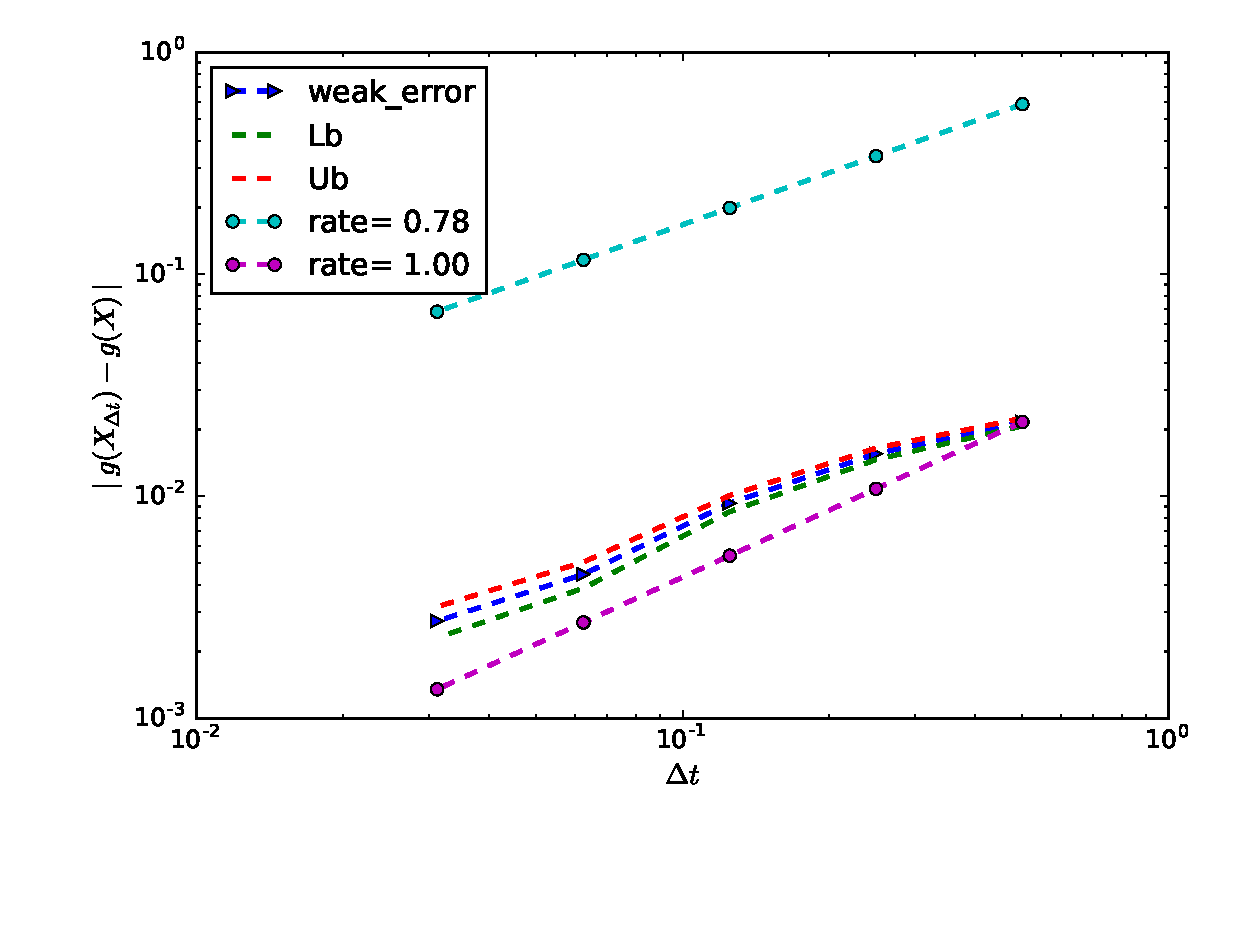
\includegraphics[width=1\linewidth]{./figures/weak_error_rates_call/Beta_32/without_rich/weak_convergence_order_call_option_relative_M_10_5}
		\caption{}
		\label{fig:sub3}
	\end{subfigure}%
	\begin{subfigure}{.35\textwidth}
		\centering
		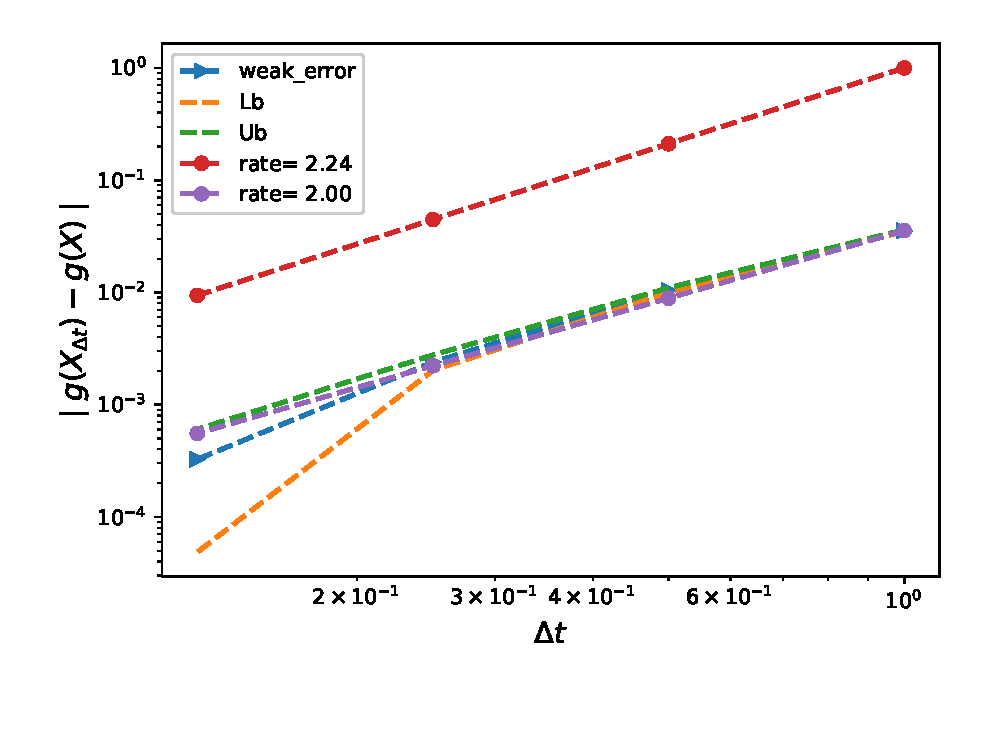
\includegraphics[width=1\linewidth]{./figures/weak_error_rates_call/Beta_32/with_rich/weak_convergence_order_call_richardson_relative}
		\caption{}
		\label{fig:sub4}
	\end{subfigure}
	
	\caption{The rate of convergence of the weak error for the call option using MC. a) $\abs{\expt{g(X_{\Delta t})}-g(X)}$  b)$\abs{\expt{2 g(X_{\Delta t/2}) -g(X_{\Delta t})}-g(X)}$ }
	\label{fig:Weak_rate_call_beta_32}
\end{figure}

%\begin{figure}[h!]
%	\centering
%	\begin{subfigure}{.35\textwidth}
%		\centering
%		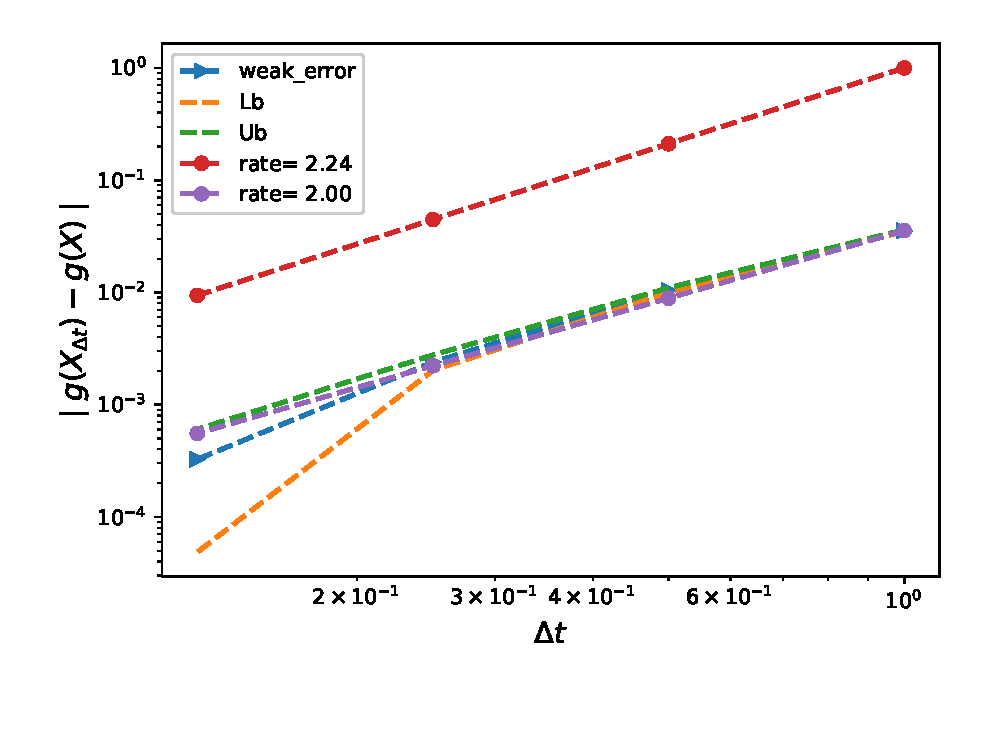
\includegraphics[width=1\linewidth]{./figures/weak_error_rates_call/Beta_32/with_rich/weak_convergence_order_call_richardson_relative}
%		\caption{}
%		\label{fig:sub3}
%	\end{subfigure}%
%	\begin{subfigure}{.35\textwidth}
%		\centering
%		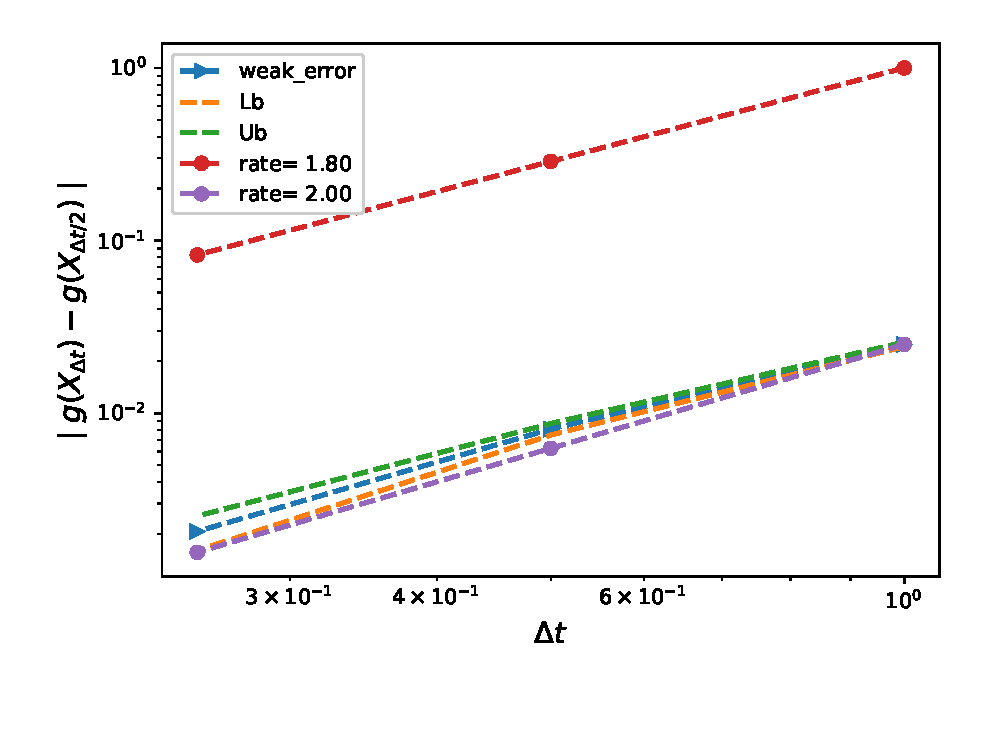
\includegraphics[width=1\linewidth]{./figures/weak_error_rates_call/Beta_32/with_rich/weak_convergence_order_differences_call_richardson_relative}
%		\caption{}
%		\label{fig:sub4}
%	\end{subfigure}
%	
%	\caption{The rate of convergence of the weak error for the  call option with Richardson extraploation (level 1), using MC with $M=5.10^6$: a)   b) $\abs{\expt{3 g(X_{\Delta t/2})-g(X_{\Delta t})-2 g(X_{\Delta t/4})}}$}
%	\label{fig:Weak_rate_call_with_rich_level1_beta_32}
%\end{figure}


%\begin{figure}[h!]
%	\centering
%	\begin{subfigure}{.4\textwidth}
%		\centering
%		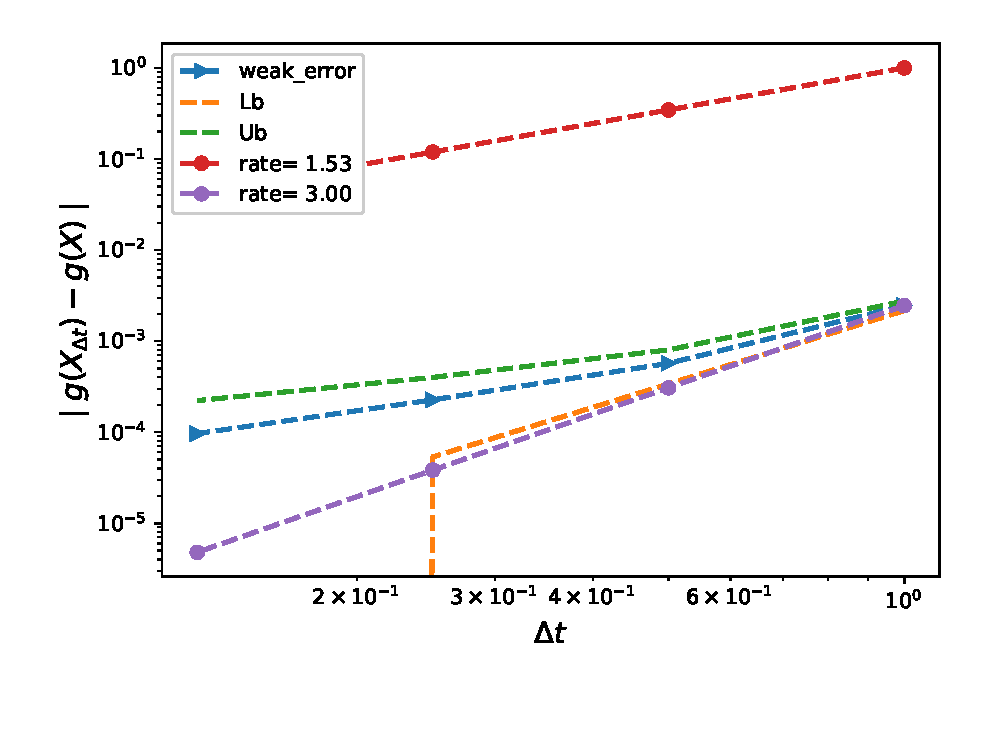
\includegraphics[width=1\linewidth]{./figures/weak_error_rates_call/Beta_32/with_rich/weak_convergence_order_Call_richardson_level2_relative_M_5_10_6}
%		\caption{}
%		\label{fig:sub3}
%	\end{subfigure}%
%	\begin{subfigure}{.4\textwidth}
%		\centering
%		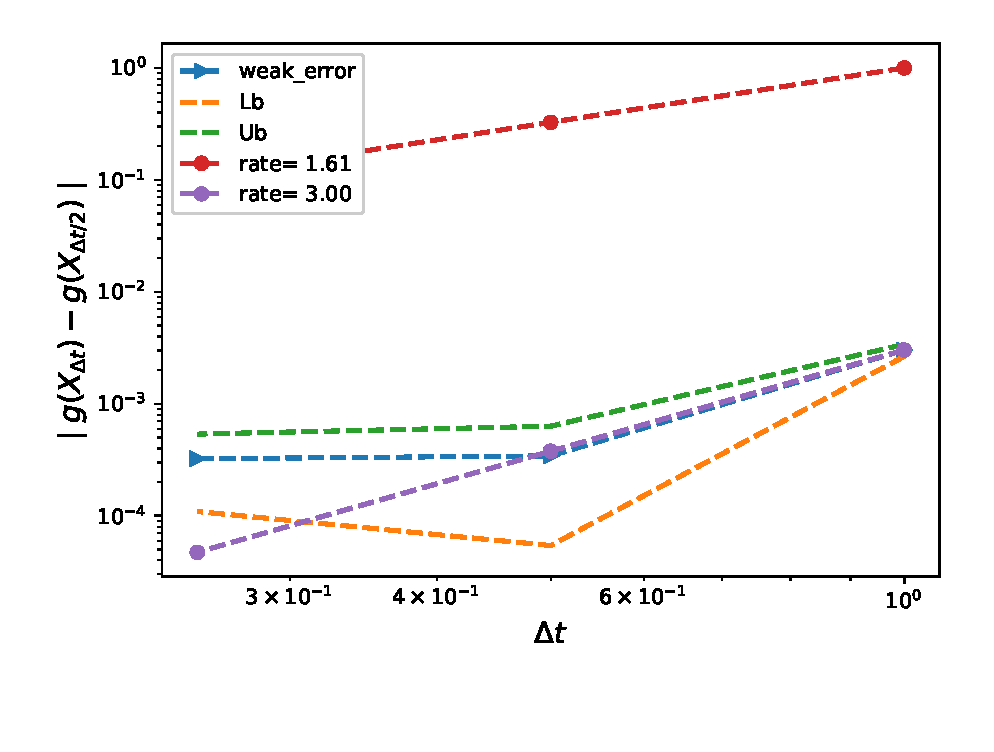
\includegraphics[width=1\linewidth]{./figures/weak_error_rates_call/Beta_32/with_rich/weak_convergence_order_differences_Call_richardson_level2_relative_M_5_10_6}
%		\caption{}
%		\label{fig:sub4}
%	\end{subfigure}
%	
%	\caption{The rate of convergence of the weak error for the  call option with Richardson extraploation (level 2), using MC with $M=5.10^6$: a) $\abs{\frac{1}{3}\expt{8 g(X_{\Delta t/4}) -6g(X_{\Delta t/2}) +g(X_{\Delta t})}-g(X)}$  b) $\abs{\frac{1}{3}\expt{-8 g(X_{\Delta t/8}) +14g(X_{\Delta t/4})-7 (X_{\Delta t/2}) +g(X_{\Delta t})}}$}
%	\label{fig:Weak_rate_call_with_rich_level2_beta_32}
%\end{figure}

\FloatBarrier
\subsubsection{Comparing relative errors}\label{sec:Comparing relative errors, call}
\subsubsection*{Without Richardson extrapolation}


%
%In this Section, we report the results for the Call option, using the different Methods: MISC, MC $+$ root finding  and MC, without Richardson extrapolation . We mention that for MISC we used a very small tolerance for the Newton solver, when solving the Kink point problem ($TOL_{\text{Newton}}=10^{-10}$), we also used $\beta=32$ (number of Laguerre quadrature points ). We start by reporting the observed approximated values using different methods (See table \ref{table:Call option price of the different methods for different number of time steps, without Richardson extrapolation.}). The biased values for MC method were computed using the values of Bias, reported in table \ref{Bias and Statistical errors of MC  for computing Call option price  for different number of time steps, without Richardson extrapolation. The numbers between parentheses are the corresponding absolute errors.}. In table \ref{Quadrature error of MISC to compute Call option price of the different tolerances for different number of time steps, without Richardson extrapolation. The numbers between parentheses are the corresponding absolute errors.}, we report the behavior of quadrature error with respect to MISC tolerance. We precise that the quadrature error is computed by substracting the MISC approximated value from the biased MC value. We report in red the values where MISC becomes stable (see also figure \ref{fig:Quadrature_error_non_rich_Call}). Those values where used to compute the needed number of samples for MC (with and without root finding), to achieve similar magnitude  for statistical error. Later, in table \ref{Total error of MISC and MC to compute Call option price of the different tolerances for different number of time steps, without Richardson extrapolation. The numbers between parentheses are the corresponding absolute errors.}, we report the total relative error for all methods (Quadrature error + Bias for MISC and Statistical error + Bias for MC). We also report in table \ref{Comparsion of the computational time of  MC and MISC, used to compute Call option price  for different number of time steps, without Richardson extrapolation}, the computational time needed for all different methods.  We finally provide in figure \ref{fig:Complexity plot for MC and MISC , Call non rich}, the complexity rates for the different involved methods.

\begin{table}[h!]
	\centering
	\begin{tabular}{l*{6}{c}r}
		Method \textbackslash  Steps            & $2$ & $4$ & $8$ & $16$ &   \\
		\hline
		MISC ($TOL_{\text{MISC}}=5.10^{-1},\beta=32$)  & $16.184$ & $16.070$ & $15.998$ & $15.930$  \\
		MISC ($TOL_{\text{MISC}}=10^{-1},\beta=32$)  & $16.184$ & $16.070$ & $15.996$ &$15.928$  \\
		MISC ($TOL_{\text{MISC}}=5.10^{-2},\beta=32$) & $16.184$ & $16.070$ & $15.996$ & $15.928$  \\
		MISC ($TOL_{\text{MISC}}=10^{-2},\beta=32$) & $16.184$ & $16.103$ & $15.996$ &$15.928$  \\
%		MISC ($TOL_{\text{MISC}}=10^{-3},\beta=32$) & $16.184$ & $16.103$ & $15.996$ & $-$  \\
		
		\hline
		MC method ($M=10^{5}$)   & $  16.194$ & $ 16.099$ & $
		15.999$ & $  15.923$  \\
		\hline
	\end{tabular}
	\caption{Call option price of the different methods for different number of time steps, without Richardson extrapolation.}
	\label{table:Call option price of the different methods for different number of time steps, without Richardson extrapolation.}
\end{table}


\begin{table}[h!]
	\centering
	\begin{tabular}{l*{6}{c}r}
		Method \textbackslash  Steps            & $2$ & $4$ & $8$ & $16$  \\
		\hline
		MC Bias ($M=10^{5}$)  & 	$ \underset{(      0.3424 )}{\mathbf{0.0216}}$  & $\underset{(0.2473)}{\mathbf{ 0.0156
		}}$  & $\underset{(  0.1474)}{\mathbf{0.0093}}$ & $\underset{(     0.0713
	)}{\mathbf{  0.0045 }}$\\ 
		
		MC Statistical error  ($M=10^{5}$)   & 	$ \underset{( 7.5e-03  )}{\mathbf{4.4e-04}}$  & $\underset{(7.5e-03 )}{\mathbf{ 4.7e-04
		}}$  & $\underset{(6.3e-03 )}{\mathbf{4.0e-04}}$ & $\underset{( 4.9e-03 )}{\mathbf{ 3.1e-04  }}$\\ 
	
%		MC Statistical error ($M=10^4$)     & 	$ \underset{( 2.2e-02  )}{\mathbf{1.4e-03}}$  & 	$ \underset{( 2.2e-02  )}{\mathbf{1.4e-03}}$  & $\underset{(1.9e-02 )}{\mathbf{1.2e-03}}$ & $\underset{( 1.5e-02 )}{\mathbf{ 9.3e-04  }}$\\ 
%		
		\hline
	\end{tabular}
	\caption{Bias and statistical errors of MC  for computing call option price  for different number of time steps, without Richardson extrapolation. The numbers between parentheses are the corresponding absolute errors.}
	\label{Bias and Statistical errors of MC  for computing Call option price  for different number of time steps, without Richardson extrapolation. The numbers between parentheses are the corresponding absolute errors.}
\end{table}




\begin{table}[h!]
	\centering
	\begin{tabular}{l*{6}{c}r}
		Method \textbackslash  Steps            & $2$ & $4$ & $8$ & $16$  \\
		\hline
		MISC ($TOL_{\text{MISC}}=5.10^{-1}$)  & $\underset{( 0.0103)}{\mathbf{\red{0.0007}}}$ & $\underset{(0.0290)}{\mathbf{0.0018}}$  & $\underset{(0.0010
			)}{\mathbf{6.3e-05}}$ &$\underset{(   0.0070)}{\mathbf{0.0004}}$ \\
		MISC ($TOL_{\text{MISC}}=10^{-1}$)   &  $\underset{( 0.0103)}{\mathbf{0.0007}}$& $\underset{(0.0290)}{\mathbf{0.0018}}$ & $\underset{(
			0.0030
			)}{\mathbf{\red{0.0002}}}$ &$\underset{(0.0020)}{\mathbf{\red{0.0001}}}$ \\
		MISC ($TOL_{\text{MISC}}=5.10^{-2}$)  &$\underset{( 0.0103)}{\mathbf{0.0007}}$ & $\underset{(0.0290)}{\mathbf{0.0018}}$  & $\underset{(
			0.0030
			)}{\mathbf{0.0002}}$ &$\underset{(0.0020)}{\mathbf{0.0001}}$ \\
		MISC ($TOL_{\text{MISC}}=10^{-2}$)  & $\underset{( 0.0103)}{\mathbf{0.0007}}$ & $\underset{( 0.0040)}{\mathbf{\red{0.0003}}}$  & $\underset{(
			0.0030
			)}{\mathbf{0.0002}}$ &$\underset{(0.0020)}{\mathbf{0.0001}}$ \\
%		MISC ($TOL_{\text{MISC}}=10^{-3}$)  & $\underset{( 0.0103)}{\mathbf{0.0007}}$  & $\underset{( 0.0040)}{\mathbf{0.0003}}$ & $\underset{(
%			0.0030
%			)}{\mathbf{0.0002}}$ &$\underset{(-)}{\mathbf{-}}$ \\
%		
		\hline
	\end{tabular}
	\caption{Quadrature error of MISC, with different tolerances, to compute call option price for different number of time steps, without Richardson extrapolation. The numbers between parentheses are the corresponding absolute errors. The values marked in red correspond to stable quadrature errors for MISC, and will be used for complexity comparison against MC.}
	\label{Quadrature error of MISC to compute Call option price of the different tolerances for different number of time steps, without Richardson extrapolation. The numbers between parentheses are the corresponding absolute errors.}
\end{table}

\FloatBarrier
	\begin{figure}[h!]
\centering
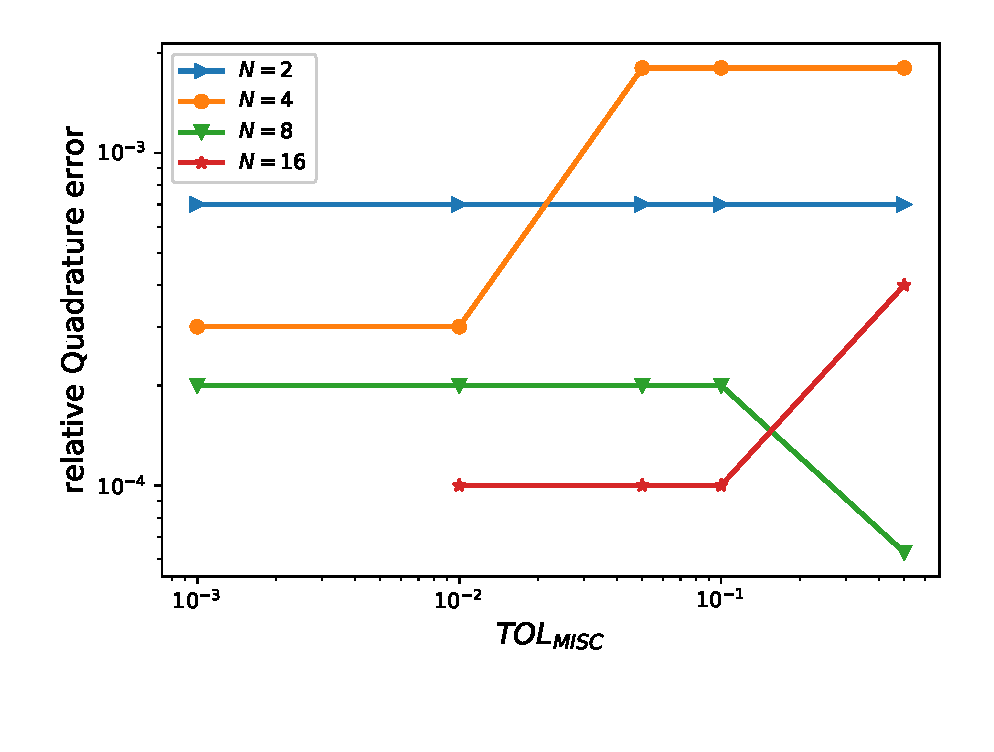
\includegraphics[width=0.4\linewidth]{./figures/Call_MISC_quadrature_error/relative_quad_error_wrt_MISC_TOL_non_rich}


\caption{Relative quadrature error of MISC, with different tolerances, to compute call option price for different number of time steps, without Richardson extrapolation.}
\label{fig:Quadrature_error_non_rich_Call}
\end{figure}


\FloatBarrier
\begin{table}[h!]
	\centering
	\begin{tabular}{l*{6}{c}r}
		Method \textbackslash  Steps            & $2$ & $4$ & $8$ & $16$  \\
		\hline
		MISC ($TOL_{\text{MISC}}=5.10^{-1}$)  &  $\mathbf{\red{0.0223}}$ & $\mathbf{0.0174}$ & $\mathbf{0.0094}$ & $\mathbf{0.0049}$  \\
		MISC ($TOL_{\text{MISC}}=10^{-1}$)  &  $\mathbf{0.0223}$& $\mathbf{0.0174}$ & $\mathbf{\red{0.0095}}$ & $\mathbf{\red{0.0046}}$  \\
		MISC ($TOL_{\text{MISC}}=5.10^{-2}$) & $\mathbf{0.0223}$ & $\mathbf{0.0174}$ &  $\mathbf{0.0095}$ & $\mathbf{0.0046}$  \\
		MISC ($TOL_{\text{MISC}}=10^{-2}$)  &  $\mathbf{0.0223}$& $\mathbf{\red{0.0159}}$ & $\mathbf{0.0095}$ &  $\mathbf{0.0046}$  \\
%		MISC ($TOL_{\text{MISC}}=10^{-3}$) &  $\mathbf{0.0223}$ & $\mathbf{0.0159}$ & $\mathbf{0.0095}$ & $\mathbf{}$  \\
		
		\hline
%		MC  ($M=10^5$)   &  $\mathbf{0.0266}$ & $\mathbf{0.0161}$ & $\mathbf{0.0097}$ & $\mathbf{\red{0.0048}}$  \\	
		
			MC +root finding  &  $\mathbf{\red{0.0223}}$ & $\mathbf{\red{0.0159}}$ & $\mathbf{\red{0.0095}}$ & $\mathbf{\red{0.0046}}$  \\	
				MC   &  $\mathbf{\red{0.0223}}$ & $\mathbf{\red{0.0159}}$ & $\mathbf{\red{0.0095}}$ & $\mathbf{\red{0.0046}}$  \\	
		\hline
	\end{tabular}
	\caption{Total relative  error of MISC, with different tolerances, and MC to compute call option price for different number of time steps, without Richardson extrapolation. The values marked in red, for MISC method, correspond to the total relative errors associated with  stable quadrature errors for MISC, and will be used for complexity comparison against MC.}
	\label{Total error of MISC and MC to compute Call option price of the different tolerances for different number of time steps, without Richardson extrapolation. The numbers between parentheses are the corresponding absolute errors.}
\end{table}

\FloatBarrier




\begin{table}[h!]
	\centering
	\begin{tabular}{l*{6}{c}r}
		Method \textbackslash  Steps            & $2$ & $4$ & $8$ & $16$ &   \\
		\hline
		MISC ($TOL_{\text{MISC}}=5.10^{-1}$) & $\red{0.3}$ & $3$ & $17$ & $473$  \\
		MISC ($TOL_{\text{MISC}}=10^{-1}$)  & $0.3$ & $3$ & $\red{58}$ & $\red{656}$  \\
		MISC ($TOL_{\text{MISC}}=5.10^{-2}$)   & $0.3$ & $3$ & $73$ & $731$  \\
		MISC ($TOL_{\text{MISC}}=10^{-2}$)  & $0.3$ & $\red{6}$ & $108$ & $1972$  \\
%		MISC ($TOL_{\text{MISC}}=10^{-3}$)   & $0.3$ & $28$ & $264$ & $-$  \\
		\hline
%		MC method ($M=10^5, \beta=32$)    & $168$ & $216$ & $290$ & $\red{432}$  \\
			MC method +root finding   & $\red{1328}$ & $\red{8140}$ & $\red{21400}$ & $\red{70200}$  \\
				MC method & $\red{1450}$ & $\red{9990}$ & $\red{32790}$ & $\red{ 158108
				}$  \\
		\hline
		
			Ratio of	$\text{(MC+root finding)}/\text{(MISC)}$ & $\red{ 4400}$ & $\red{   1400}$ & $\red{369}$ & $\red{ 107}$  \\
		Ratio of	$(\text{MC})/(\text{MISC})$ & $\red{ 4800}$ & $\red{ 1665}$ & $\red{ 565}$ & $\red{ 241}$  \\
		\hline
	\end{tabular}
	\caption{Comparison of the computational time of  MC and MISC, used to compute call option price  for different number of time steps, without Richardson extrapolation. The average computational time of MC is computed over $10$ runs.}
	\label{Comparsion of the computational time of  MC and MISC, used to compute Call option price  for different number of time steps, without Richardson extrapolation}
\end{table}



\FloatBarrier
	\begin{figure}[h!]
\centering
\includegraphics[width=0.4\linewidth]{./figures/Call_Complexity_rates/error_vs_time}

\caption{Complexity plot for MC and MISC for the case without Richardson extrapolation.}
\label{fig:Complexity plot for MC and MISC , Call non rich}
\end{figure}


\FloatBarrier

\subsubsection*{With Richardson extrapolation (level $1$)}



%%
%%In this Section, we report the results for the Call option, using the different Methods: MISC, MC $+$ root finding  and MC, with Richardson extrapolation . We mention that for MISC we used a very small tolerance for the Newton solver, when solving the Kink point problem ($TOL_{\text{Newton}}=10^{-10}$), we also used $\beta=32$ (number of Laguerre quadrature points ). We start by reporting the observed approximated values using different methods (See table \ref{table: Call option price of the different methods for different number of time steps, with Richardson extrapolation (level1).}. The biased values for MC method were computed using the values of Bias, reported in table \ref{Bias and Statistical errors of MC  for computing Call option price  for different number of time steps, with Richardson extrapolation (level $1$). The numbers between parentheses are the corresponding absolute errors.}. In table \ref{Quadrature error of MISC to compute Call option price of the different tolerances for different number of time steps, with Richardson extrapolation (level $1$). The numbers between parentheses are the corresponding absolute errors.}, we report the behavior of quadrature error with respect to MISC tolerance. We precise that the quadrature error is computed by substracting the MISC approximated value from the biased MC value. We report in red the values where MISC becomes stable (see also figure \ref{fig:Quadrature_error_with_rich_Call}). Those values where used to compute the needed number of samples for MC (with and without root finding), to achieve similar magnitude  for statistical error. Later, in table \ref{Total error of MISC and MC to compute Call option price of the different tolerances for different number of time steps, with Richardson extrapolation (level $1$). The numbers between parentheses are the corresponding absolute errors.}, we report the total relative error for all methods (Quadrature error + Bias for MISC and Statistical error + Bias for MC). We also report in table\ref{Comparsion of the computational time of  MC and MISC, used to compute Call option price  for different number of time steps, with Richardson extrapolation (level $1$)}, the computational time needed for all different methods.  We finally provide in figure \ref{fig:Complexity plot for MC and MISC , Call, comparison}, the comparison between the two versions of MISC (without/with Richardson extrapolation).



\begin{table}[h!]
	\centering
	\begin{tabular}{l*{6}{c}r}
		Method \textbackslash  Steps            & $1-2$ & $2-4$ & $4-8$ & $8-16$ &   \\
		\hline
		MISC ($TOL_{\text{MISC}}=5.10^{-1}$)  & $16.4108$ & $16.0254$ & $15.8912$ & $15.8621$  \\
		MISC ($TOL_{\text{MISC}}=10^{-1}$)  & $16.4108$ & $16.0254$ & $15.8883$ & $15.8603$  \\
		MISC ($TOL_{\text{MISC}}=5.10^{-2}$) & $16.4108$ & $16.0218$ & $15.8885$ & $15.8600$  \\
%		MISC ($TOL_{\text{MISC}}=10^{-2}$) & $16.4108$& $16.0218$ & $15.8888$ & $15.8595$  \\
%		MISC ($TOL_{\text{MISC}}=10^{-3}$) & $16.4108$ & $16.0207$ & $15.8885$ & $-$  \\
		
		\hline
		MC method ($M=5.10^{6}$)   & $  16.4147$ & $ 16.0184$ & $15.8900$ & $15.8567$  \\
		\hline
	\end{tabular}
	\caption{Call option price of the different methods for different number of time steps, with Richardson extrapolation (level $1$).}
	\label{table: Call option price of the different methods for different number of time steps, with Richardson extrapolation (level1).}
\end{table}


\begin{table}[h!]
	\centering
	\begin{tabular}{l*{6}{c}r}
		Method \textbackslash  Steps            & $1-2$ & $2-4$ & $4-8$ & $8-16$  \\
		\hline
		MC Bias ($M=5.10^6$)   & 	$ \underset{(    0.5627
			 )}{\mathbf{0.0355}}$  & $\underset{(  0.1664)}{\mathbf{ 0.0105
		}}$  & $\underset{( 0.0380)}{\mathbf{0.0024}}$ & $\underset{( 0.0048
	 )}{\mathbf{ 0.0003  }}$\\ 
		
		MC Statistical error ($M=5.10^6$)     & 	$ \underset{(  4.4e-03 )}{\mathbf{2.8e-04}}$  & $\underset{(3.8e-03 )}{\mathbf{ 2.4e-04
		}}$  & $\underset{(3.0e-03)}{\mathbf{1.9e-04}}$ & $\underset{(2.2e-03 )}{\mathbf{ 1.4e-04  }}$\\ 
		
%			MC Statistical error ($M=10^5$)     & 	$ \underset{(  1.4e-02 )}{\mathbf{9.0e-04}}$  & $\underset{(1.3e-02)}{\mathbf{ 8.0e-04
%		}}$  & $\underset{(9.4e-03)}{\mathbf{5.9e-04}}$ & $\underset{( 7.1e-03 )}{\mathbf{ 4.5e-04  }}$\\ 
		\hline
	\end{tabular}
	\caption{Bias and statistical errors of MC  for computing Call option price  for different number of time steps, with Richardson extrapolation (level $1$). The numbers between parentheses are the corresponding absolute errors.}
	\label{Bias and Statistical errors of MC  for computing Call option price  for different number of time steps, with Richardson extrapolation (level $1$). The numbers between parentheses are the corresponding absolute errors.}
\end{table}




\begin{table}[h!]
	\centering
	\begin{tabular}{l*{6}{c}r}
		Method \textbackslash  Steps            & $1-2$ & $2-4$ & $4-8$ & $8-16$  \\
		\hline
		MISC ($TOL_{\text{MISC}}=5.10^{-1}$)  & $\underset{(0.0039
			)}{\mathbf{ \red{2.5e-04}}}$ & $\underset{(0.0070)}{\mathbf{4.4e-04}}$  & $\underset{(0.0012
			)}{\mathbf{7.6e-05}}$ &$\underset{(0.0054)}{\mathbf{3.4e-04}}$ \\
		MISC ($TOL_{\text{MISC}}=10^{-1}$)   & $\underset{(0.0039
			)}{\mathbf{ 2.5e-04}}$ & $\underset{(0.0070)}{\mathbf{4.4e-04}}$  & $\underset{(  0.0017)}{\mathbf{1.1e-04}}$ &$\underset{(0.0036)}{\mathbf{\red{2.3e-04}}}$ \\
		MISC ($TOL_{\text{MISC}}=5.10^{-2}$)  & $\underset{(0.0039
			)}{\mathbf{ 2.5e-04}}$ & $\underset{(0.0034)}{\mathbf{\red{\red{2.1e-04}}}}$  & $\underset{(    0.0015)}{\mathbf{\red{9.5e-05}}}$ &$\underset{(0.0033)}{\mathbf{2.1e-04}}$ \\
%		MISC ($TOL_{\text{MISC}}=10^{-2}$)  & $\underset{(0.0039
%			)}{\mathbf{ 2.5e-04}}$ & $\underset{(0.0034)}{\mathbf{2.1e-04}}$  & $\underset{(0.0012
%			)}{\mathbf{7.6e-05}}$&$\underset{(0.0028
%			)}{\mathbf{1.7e-04}}$ \\
%		MISC ($TOL_{\text{MISC}}=10^{-3}$)  & $\underset{(0.0039
%			)}{\mathbf{ 2.5e-04}}$ & $\underset{(0.0023
%			)}{\mathbf{1.5e-04}}$   &$\underset{(    0.0015)}{\mathbf{9.5e-05}}$ & $\underset{()}{\mathbf{}}$ \\
		
		\hline
	\end{tabular}
	\caption{Quadrature error of MISC, with different tolerances, to compute call option price  for different number of time steps, with Richardson extrapolation (level $1$). The numbers between parentheses are the corresponding absolute errors. The values marked in red correspond to stable quadrature errors for MISC, and will be used for complexity comparison against MC.}
	\label{Quadrature error of MISC to compute Call option price of the different tolerances for different number of time steps, with Richardson extrapolation (level $1$). The numbers between parentheses are the corresponding absolute errors.}
\end{table}

\FloatBarrier


	\begin{figure}[h!]
\centering
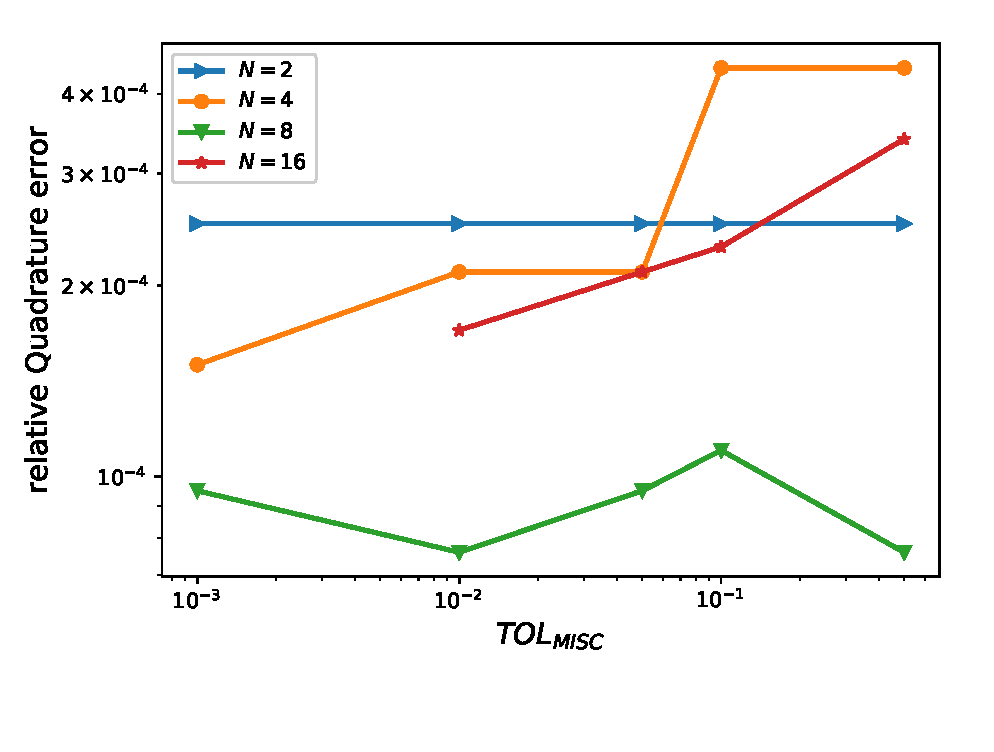
\includegraphics[width=0.4\linewidth]{./figures/Call_MISC_quadrature_error/relative_quad_error_wrt_MISC_TOL_with_rich}


\caption{Relative quadrature error of MISC, with different tolerances, to compute call option price for different number of time steps, with Richardson extrapolation.}
\label{fig:Quadrature_error_with_rich_Call}
\end{figure}




\FloatBarrier

\begin{table}[h!]
	\centering
	\begin{tabular}{l*{6}{c}r}
		Method \textbackslash  Steps            & $1-2$ & $2-4$ & $4-8$ & $8-16$  \\
		\hline
		MISC ($TOL_{\text{MISC}}=5.10^{-1}$)  &  $\mathbf{\red{0.0358}}$ & $\mathbf{0.0109}$ & $\mathbf{0.0025}$ & $\mathbf{0.0006}$  \\
		MISC ($TOL_{\text{MISC}}=10^{-1}$)  &  $\mathbf{0.0358}$ & $\mathbf{0.0109}$ & $\mathbf{0.0025}$ & $\mathbf{\red{0.0005}}$  \\
		MISC ($TOL_{\text{MISC}}=5.10^{-2}$) &  $\mathbf{0.0358}$ & $\mathbf{\red{0.0107}}$ & $\mathbf{\red{0.0025}}$ & $\mathbf{0.0005}$  \\
%		MISC ($TOL_{\text{MISC}}=10^{-2}$)  &  $\mathbf{0.0358}$ & $\mathbf{0.0107}$ & $\mathbf{0.0025}$ & $\mathbf{0.0005}$ \\
%		MISC ($TOL_{\text{MISC}}=10^{-3}$) &  $\mathbf{0.0358}$ & $\mathbf{0.0107}$ & $\mathbf{0.0025}$ & $\mathbf{}$  \\
		
		\hline
%		MC  ($M=5.10^6$)   &  $\mathbf{\red{0.0358}}$ & $\mathbf{\red{0.0107}}$ & $\mathbf{\red{0.0026}}$ & $\mathbf{\red{0.0004}}$  \\	
%			MC + root finding  &  $\mathbf{\red{0.0358}}$ & $\mathbf{\red{0.0107}}$ & $\mathbf{\red{0.0025}}$ & $\mathbf{\red{0.}}$  \\	
		\hline
	\end{tabular}
	\caption{Total relative error of MISC, with different tolerances,  to compute call option price for different number of time steps, with Richardson extrapolation (level $1$).  The values marked in red, for MISC method, correspond to the total relative errors associated with  stable quadrature errors for MISC, and will be used for complexity comparison against MC.}
	\label{Total error of MISC and MC to compute Call option price of the different tolerances for different number of time steps, with Richardson extrapolation (level $1$). The numbers between parentheses are the corresponding absolute errors.}
\end{table}



\FloatBarrier


\begin{table}[h!]
	\centering
	\begin{tabular}{l*{6}{c}r}
		Method \textbackslash  Steps            & $1-2$ & $2-4$ & $4-8$ & $8-16$ &   \\
		\hline
		MISC ($TOL_{\text{MISC}}=5.10^{-1}$) & $\red{0.3}$ & $4$ & $56$ & $713$  \\
		MISC ($TOL_{\text{MISC}}=10^{-1}$)  & $0.3$  & $4$ & $107$ & $\red{1126}$  \\
		MISC ($TOL_{\text{MISC}}=5.10^{-2}$)   & $0.3$  & $\red{9}$ & $\red{135}$ & $1253$  \\
%		MISC ($TOL_{\text{MISC}}=10^{-2}$)  &  $0.3$  & $9$ & $186$ & $3540$  \\
%		MISC ($TOL_{\text{MISC}}=10^{-3}$)   & $0.3$  & $63$ & $836$ & $$  \\
		\hline
%		MC +root finding   & $\red{ 2.4e+05}$ & $\red{ 4.3e+05}$ & $\red{ 3.5e+06}$ & $\red{-}$  \\
		\hline
	\end{tabular}
	\caption{Comparison of the computational time of  MISC, used to compute call option price  for different number of time steps, with Richardson extrapolation (level $1$). The average computational time of MC is computed over $10$ runs.}
	\label{Comparsion of the computational time of  MC and MISC, used to compute Call option price  for different number of time steps, with Richardson extrapolation (level $1$)}
\end{table}


\FloatBarrier
%	\begin{figure}[h!]
%	\centering
%	\includegraphics[width=0.7\linewidth]{./figures/Call_Complexity_rates/error_vs_time_rich}
%	
%	\caption{Complexity plot for MC and MISC for the case with Richardson extrapolation.}
%	\label{fig:Complexity plot for MC and MISC , Call, with rich}
%\end{figure}







\begin{figure}[h!]
	\centering
	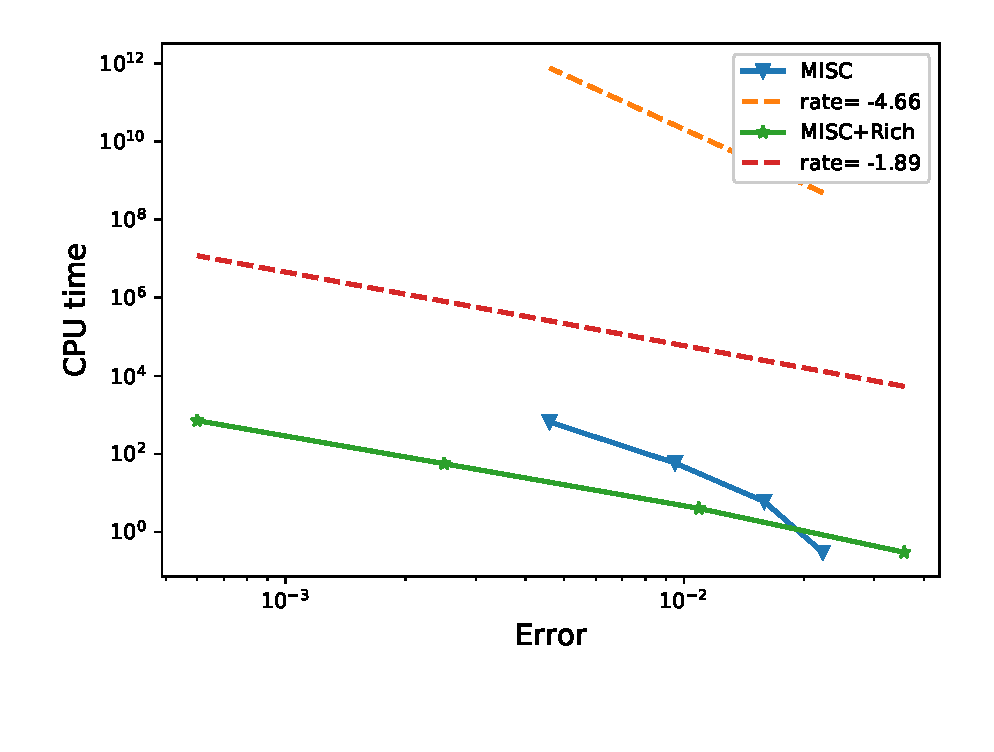
\includegraphics[width=0.4\linewidth]{./figures/Call_Complexity_rates/error_vs_time_comparision}
	
	\caption{Complexity plot for MISC without and with Richardson extrapolation, for the call option.}
	\label{fig:Complexity plot for MC and MISC , Call, comparison}
\end{figure}




\FloatBarrier
%In the following, we compare the  relative errors for the call option example under Black-Scholes model(see Tables (\ref{Relative error of the call option price of the different tolerances for different number of time steps.}, \ref{Relative error of Call option price of the different tolerances for different number of time steps, using Richardson extrapolation (level $1$)}, \ref{Relative error of Call option price of the different tolerances for different number of time steps, using Richardson extrapolation (level $2$)})). We report the results for $3$ scenarios: i) Without using Richardson extrapolation, ii) Using level $1$ Richardson extrapoaltion, iii) Using level $2$ Richardson extrapoaltion.  You may see appendix \ref{appendix:Call prices for different methods} for the values of call option prices. The value of $\beta$ used to get those points is $\beta=10$.
%
%Given the normalized bias computed by MC method (See Section \ref{sec:Weak error plots_call}) (reported as bold values in the tables), we report in red in each table the smallest tolerance that MISC required to get below that relative bias (I do not put values for smaller tolerances, once the required bias is reached). In case I do not reach those bias I put the best value that I get with MISC in red.
%
%From the tables (\ref{Relative error of the call option price of the different tolerances for different number of time steps.}, \ref{Relative error of Call option price of the different tolerances for different number of time steps, using Richardson extrapolation (level $1$)}, \ref{Relative error of Call option price of the different tolerances for different number of time steps, using Richardson extrapolation (level $2$)})), we may observe that to get a relative error below $0.5\%$, we need more than $16$ time steps for the case without Richardson extrapolation compared to only using $4$ time step in the coarse level for the case of level $1$ Richardson extraplation,  and  only using $1$ time step in the coarse level for the case of level $2$ Richardson extraplation.

%\begin{table}[h!]
%	\centering
%	\begin{tabular}{l*{6}{c}r}
%		Method \textbackslash  Steps            & $2$ & $4$ & $8$ & $16$ &   \\
%		\hline
%		MISC ($TOL_{\text{MISC}}=5.10^{-1}$)  & $ \red{0.0229}$ & $  0.0179$ & $\red{0.0111}$ & $ 0.0068$  \\
%		MISC ($TOL_{\text{MISC}}=10^{-3}$)  & $-$ & $ \red{ 0.0177}$ & $-$ & $\red{  0.0066}$  \\
%			MC method ($M=10^{5}$)&$ \mathbf{0.0231}$    & $\mathbf{0.0175}$  & $\mathbf{0.0111}$  & $\mathbf{0.0064}$ \\	
%		\hline
%	\end{tabular}
%	\caption{Relative error of the call option price of the different tolerances for different number of time steps, without Richardson extrapolation}
%	\label{Relative error of the call option price of the different tolerances for different number of time steps.}
%\end{table}

%\begin{table}[h!]
%	\centering
%	\begin{tabular}{l*{5}{c}r}
%		Method \textbackslash  Steps    &$1-2$        & $2-4$ & $4-8$ & $8-16$  \\
%		\hline
%		MISC ($TOL_{\text{MISC}}=5.10^{-1}$)  &$\red{0.0372}$ & $ 0.0129$ & $0.0043$ & $ 0.0025$  \\
%		MISC ($TOL_{\text{MISC}}=10^{-3}$) & $-$ & $ \red{0.0126}$ & $\red{    0.0042}$ & $\red{0.0023}$   \\
%		MC method ($M=10^{5}$)&$ \mathbf{0.0374}$    & $\mathbf{0.0116}$  & $\mathbf{0.0027}$  & $\mathbf{0.0022}$ \\
%		\hline
%	\end{tabular}
%	\caption{Relative error of the call option price of the different tolerances for different number of time steps, using Richardson extrapolation (level $1$)}
%	\label{Relative error of Call option price of the different tolerances for different number of time steps, using Richardson extrapolation (level $1$)}
%\end{table}


%\begin{table}[h!]
%	\centering
%	\begin{tabular}{l*{5}{c}r}
%		Method \textbackslash  Steps    &$1-2-4$        & $2-4-8$ & $4-8-16$   \\
%		\hline
%		MISC ($TOL_{\text{MISC}}=5.10^{-1}$)  &$0.0047$ & $  0.0015$ & $0.0019
%		$   \\
%		MISC ($TOL_{\text{MISC}}=10^{-3}$) & $ \red{0.0043}$ & $ \red{0.0013}$ & $\red{  0.0017}$    \\
%		MC method ($M=10^{6}$)&$ \mathbf{0.0041}$    & $\mathbf{0.0013}$  & $\mathbf{0.0016}$  \\
%		\hline
%	\end{tabular}
%	\caption{Relative error of the call option price of the different tolerances for different number of time steps, using Richardson extrapolation (level $2$)}
%	\label{Relative error of Call option price of the different tolerances for different number of time steps, using Richardson extrapolation (level $2$)}
%\end{table}








\subsection{Result for the  $2$-dimensional Basket call option}\label{sec:Result for the  $2$-dimensional Basket call option}
\subsubsection{Weak error plots} \label{sec:Weak error plots_Basket_2D_call}

We consider the case of $2$-dimensional Basket call option, with parameters: $S^{(1,2)}=100$, $K=100$, $\sigma^{(1,2)}=0.4$, $\rho=0.3$, $r=0$, $T=1$.  The MC  value of this case (with large number of samples) is $12.900784$ with a statistical error equal to $	0.001033$ (Provided by Premia).


In this section, we include the results of weak error rates for $2$ scenarios, without/with Richardson extrapolation (level $1$). We note that the weak errors plotted here correspond to relative errors.  

 We can see from figure \ref{fig:Weak_rate_basket_2d} that we get a weak error of order $\Delta t$ for the case without Richardson extrapolation and almost $\Delta t^2$ for the case with Richardson extrapolation. 
 
% From figure \ref{fig:Weak_rate_call_with_rich_level1_beta_64}, we observe an improvement in the rate and the constant when using level $1$ of Richardson extrapolation, approximately of order $\Delta t^2$. For all the plots below, the upper and lower bounds are $95\%$ confidence interval.



\begin{figure}[h!]
	\centering
	\begin{subfigure}{.35\textwidth}
		\centering
		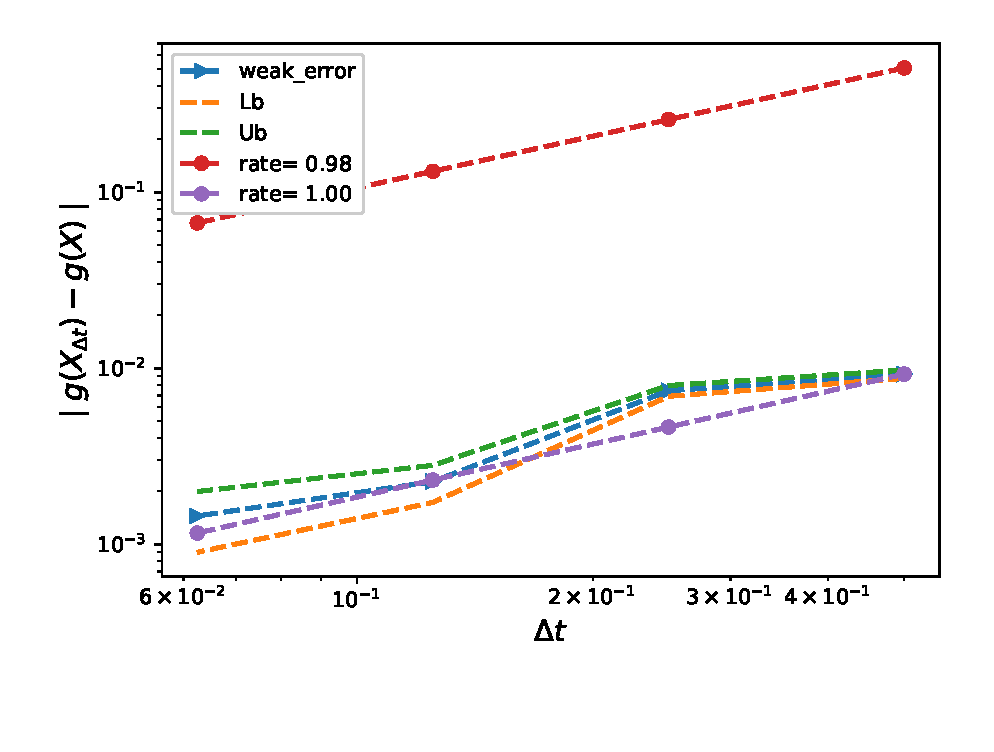
\includegraphics[width=1\linewidth]{./figures/weak_error_rates_basket_2d/without_richardson/weak_convergence_order_basket_option_2d_1_relative_M_4_10_7_plain}
		\caption{}
		\label{fig:sub3}
	\end{subfigure}%
	\begin{subfigure}{.35\textwidth}
		\centering
		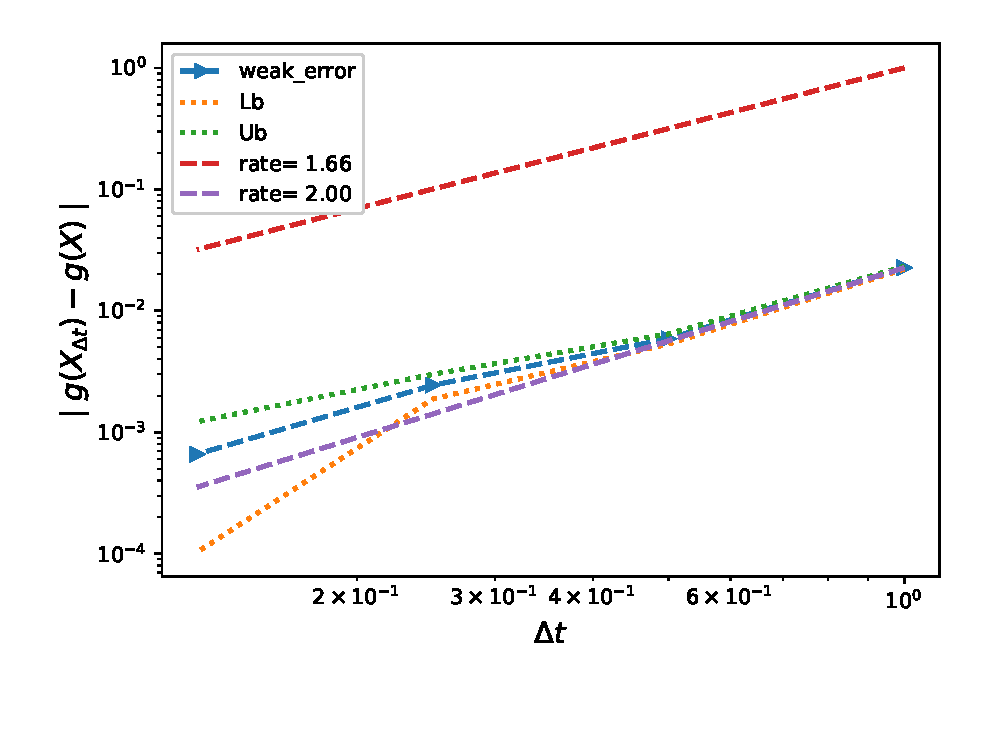
\includegraphics[width=1\linewidth]{./figures/weak_error_rates_basket_2d/with_richardson/weak_convergence_order_basket_option_2d_1_richardson_relative_M_4_10_7_plain}
		\caption{}
		\label{fig:sub4}
	\end{subfigure}
	
	\caption{The rate of convergence of the weak error for the Basket ($2$-dimensional) call option using MC. a) $\abs{\expt{g(X_{\Delta t})}-g(X)}$  b) $\abs{\expt{2 g(X_{\Delta t/2}) -g(X_{\Delta t})}-g(X)}$}
	\label{fig:Weak_rate_basket_2d}
\end{figure}






%\begin{figure}[h!]
%	\centering
%	\begin{subfigure}{.35\textwidth}
%		\centering
%		\includegraphics[width=1\linewidth]{}
%		\caption{}
%		\label{fig:sub3}
%	\end{subfigure}%
%	\begin{subfigure}{.35\textwidth}
%		\centering
%		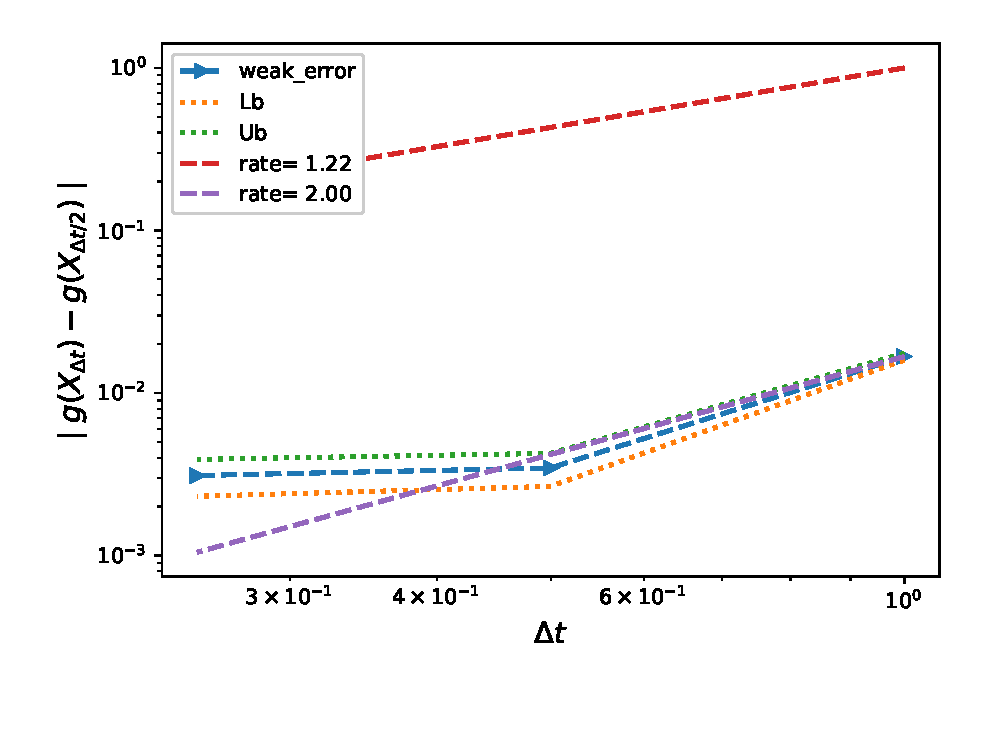
\includegraphics[width=1\linewidth]{./figures/weak_error_rates_basket_2d/with_richardson/weak_convergence_order_differences_basket_option_2d_1_richardson_relative_M_4_10_7_plain}
%		\caption{}
%		\label{fig:sub4}
%	\end{subfigure}
%	
%	\caption{The rate of convergence of the weak error for the  Basket ($2$-dimensional) call option with Richardson extraploation (level 1), using MC with $M=4.10^7$: a)   b) $\abs{\expt{3 g(X_{\Delta t/2})-g(X_{\Delta t})-2 g(X_{\Delta t/4})}}$}
%	\label{fig:Weak_rate_call_with_rich_level1}
%\end{figure}




\FloatBarrier
\subsubsection{Comparing relative errors}\label{sec:Comparing relative errors, basket call}
\subsubsection*{Without Richardson extrapolation}


\begin{table}[h!]
\centering
\begin{tabular}{l*{6}{c}r}
Method \textbackslash  Steps            & $2$ & $4$ & $8$ & $16$ &   \\
\hline
MISC ($TOL_{\text{MISC}}=5.10^{-1},\beta=16$)  & $
 13.0009$ & $    12.8577$ & $    12.8854$ & $
   12.9000$  \\
MISC ($TOL_{\text{MISC}}=10^{-1},\beta=16$)  & $
 13.0009$ & $   12.9912
$ & $
12.9556
$ &$ 12.9231$  \\
MISC ($TOL_{\text{MISC}}=5.10^{-2},\beta=16$) & $
 13.0009$ & $    13.0049
$ & $ 12.9550

$ & $-$  \\
MISC ($TOL_{\text{MISC}}=10^{-2},\beta=16$) & $  13.0548$ & $    13.0046$ & $   12.9550
$ &$-$  \\
%MISC ($TOL_{\text{MISC}}=10^{-3},\beta=16$) & $   13.0548$ & $   13.0046$ & $-$ & $-$  \\
%MISC ($TOL_{\text{MISC}}=10^{-4},\beta=16$) & $  13.0545$ & $   13.0047$ & $-$ & $-$  \\
%MISC ($TOL_{\text{MISC}}=10^{-5},\beta=16$) & $  13.0545$ & $-$ & $-$ & $-$  \\
\hline
MC method ($M=4.10^{7}$)   & $  13.0203
$ & $ 12.9969$ & $12.9301
$ & $ 12.9194 $  \\
\hline
\end{tabular}
\caption{Basket ($2$-dimensional) call option price of the different methods for different number of time steps, without Richardson extrapolation.}
\label{table:Basket 2d option price of the different methods for different number of time steps, without Richardson extrapolation, beta_16}
\end{table}







\FloatBarrier



\begin{table}[h!]
	\centering
	\begin{tabular}{l*{6}{c}r}
		Method \textbackslash  Steps            & $2$ & $4$ & $8$ & $16$  \\
		\hline
		MC Bias ($M=4.10^{7}$)  & 	$ \underset{(      0.1195
			 )}{\mathbf{0.0093}}$  & $\underset{(0.0968
			 )}{\mathbf{ 0.0075
		}}$  & $\underset{(  0.0297)}{\mathbf{0.0023}}$ & $\underset{(         0.0181
	
			)}{\mathbf{  0.0014 }}$\\ 
		
		MC Statistical error  ($M=4.10^{7}$)   & 	$ \underset{( 3.2e-03  )}{\mathbf{2.5e-04}}$  & $\underset{(3.5e-03 )}{\mathbf{ 2.7e-04
		}}$  & $\underset{(3.6e-03 )}{\mathbf{2.8e-04}}$ & $\underset{( 3.6e-03 )}{\mathbf{ 2.8e-04  }}$\\ 
		\hline
	\end{tabular}
	\caption{Bias and statistical errors of MC  for computing Basket ($2$-dimensional) call option price  for different number of time steps, without Richardson extrapolation. The numbers between parentheses are the corresponding absolute errors.}
	\label{Bias and Statistical errors of MC  for computing Basket 2d Call option price  for different number of time steps, without Richardson extrapolation. The numbers between parentheses are the corresponding absolute errors.}
\end{table}


\FloatBarrier
\begin{table}[h!]
\centering
\begin{tabular}{l*{6}{c}r}
Method \textbackslash  Steps            & $2$ & $4$ & $8$ & $16$  \\
\hline
MISC ($TOL_{\text{MISC}}=5.10^{-1}$)  & $\underset{(  0.0194)}{\mathbf{    0.0015}}$  & $\underset{(   0.1392
	)}{\mathbf{    0.0108}}$ & $\underset{( 0.0447
	
	-
	)}{\mathbf{ 0.0035}}$ &$\underset{(
	0.0194)}{\mathbf{   \red{ 0.0015}}}$ \\
MISC ($TOL_{\text{MISC}}=10^{-1}$)  & $\underset{(  0.0194)}{\mathbf{    0.0015}}$   & $\underset{(   0.0057)}{\mathbf{4.4e-04}}$ & $\underset{(0.0255)}{\mathbf{\red{0.0020}}}$ &$\underset{(0.0037)}{\mathbf{2.9e-04}}$ \\
MISC ($TOL_{\text{MISC}}=5.10^{-2}$)  & $\underset{(  0.0194)}{\mathbf{    0.0015}}$  & $\underset{( 0.0080)}{\mathbf{\red{6.2e-04}}}$ & $\underset{(
	0.0249
	)}{\mathbf{0.0019}}$ &$\underset{(-)}{\mathbf{-}}$ \\
MISC ($TOL_{\text{MISC}}=10^{-2}$)  & $\underset{( 0.0345)}{\mathbf{\red{0.0027}}}$  & $\underset{( 0.0077)}{\mathbf{6.0e-04}}$ & $\underset{(
	0.0249
	)}{\mathbf{0.0019}}$&$\underset{(-)}{\mathbf{-}}$ \\
%MISC ($TOL_{\text{MISC}}=10^{-3}$)  & $\underset{( 0.0345)}{\mathbf{0.0027}}$  & $\underset{( 0.0077)}{\mathbf{6.0e-04}}$ & $\underset{(
%-
%	)}{\mathbf{-}}$ &$\underset{(-)}{\mathbf{-}}$ \\
%MISC ($TOL_{\text{MISC}}=10^{-4}$)  & $\underset{( 0.0342)}{\mathbf{0.0027
%}}$  & $\underset{( 0.0078)}{\mathbf{6.0e-04}}$& $\underset{(
%	-
%	)}{\mathbf{-}}$ &$\underset{(-)}{\mathbf{-}}$ \\
%MISC ($TOL_{\text{MISC}}=10^{-5}$)  & $\underset{( 0.0342)}{\mathbf{0.0027
%}}$  & $\underset{( -)}{\mathbf{-}}$ & $\underset{(
%	-
%	)}{\mathbf{-}}$ &$\underset{(-)}{\mathbf{-}}$ \\
\hline
\end{tabular}
\caption{Quadrature error of MISC, with different tolerances, to compute Basket ($2$-dimensional) call option price  for different number of time steps, without Richardson extrapolation. The numbers between parentheses are the corresponding absolute errors. The values marked in red correspond to stable quadrature errors for MISC, and will be used for complexity comparison against MC.}
\label{Quadrature error of MISC to compute Basket 2d Call option price of the different tolerances for different number of time steps, without Richardson extrapolation. The numbers between parentheses are the corresponding absolute errors, beta_16}
\end{table}

\FloatBarrier
	\begin{figure}[h!]
	\centering
	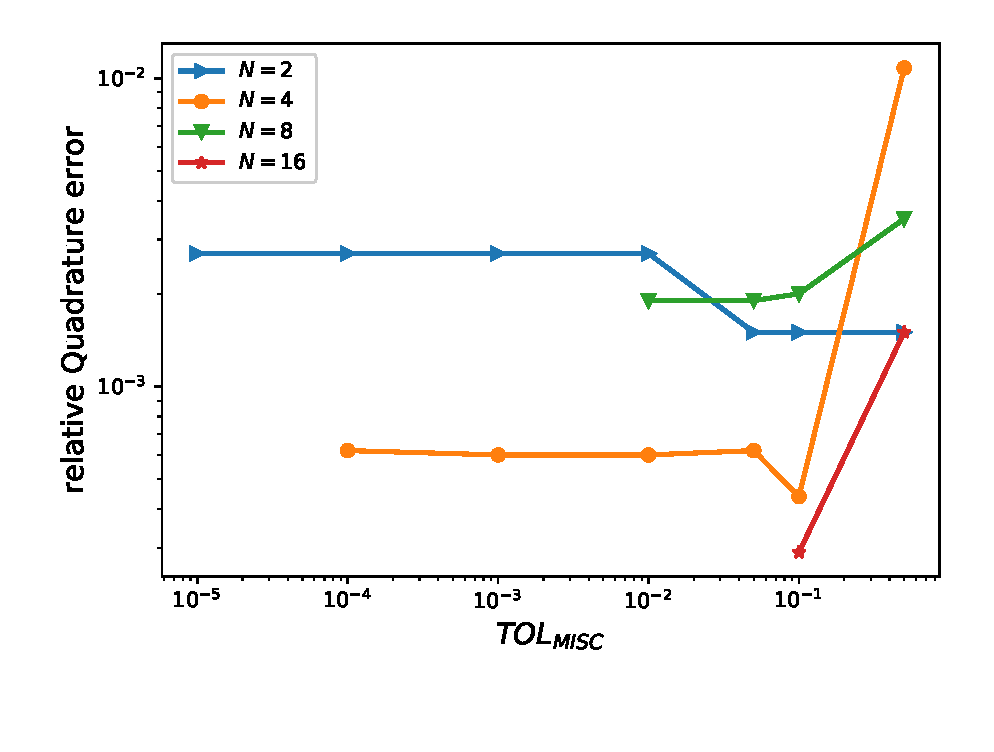
\includegraphics[width=0.4\linewidth]{./figures/Basket_2d_MISC_quadrature_error/relative_quad_error_wrt_MISC_TOL_non_rich}
	
	
	\caption{Relative quadrature error of MISC,with different tolerances,  to compute Basket ($2$-dimensional) call option price for different number of time steps, without Richardson extrapolation.}
	\label{fig:Quadrature_error_non_rich_basket_Call}
\end{figure}

\FloatBarrier

\begin{table}[h!]
	\centering
	\begin{tabular}{l*{6}{c}r}
		Method \textbackslash  Steps            & $2$ & $4$ & $8$ & $16$  \\
		\hline
		MISC ($TOL_{\text{MISC}}=5.10^{-1}$) &$\mathbf{0.0108}$ & $\mathbf{0.0183}$ & $\mathbf{0.0058}$ & $\mathbf{\red{0.0029}}$  \\	
		MISC ($TOL_{\text{MISC}}=10^{-1}$) & $\mathbf{0.0108}$ & $\mathbf{0.0079}$ & $\mathbf{\red{0.0043}}$ & $\mathbf{0.0017}$  \\	
		MISC ($TOL_{\text{MISC}}=5.10^{-2}$) & $\mathbf{0.0108}$ & $\mathbf{\red{0.0081}}$ & $\mathbf{0.0042}$ & $\mathbf{-}$  \\	
		MISC ($TOL_{\text{MISC}}=10^{-2}$)& $\mathbf{\red{0.0120}}$ & $\mathbf{0.0081}$ &$\mathbf{0.0042}$ & $\mathbf{-}$  \\	
%		MISC ($TOL_{\text{MISC}}=10^{-3}$) &  $\mathbf{0.0120}$& $\mathbf{0.0081}$ & $\mathbf{-}$ & $\mathbf{-}$  \\	
%		MISC ($TOL_{\text{MISC}}=10^{-4}$) &  $\mathbf{0.0120}$& $\mathbf{0.0081}$ & $\mathbf{-}$ & $\mathbf{-}$  \\
%		MISC ($TOL_{\text{MISC}}=10^{-5}$) &  $\mathbf{0.0120}$& $\mathbf{-}$ & $\mathbf{-}$ & $\mathbf{-}$  \\
		\hline	
		MC +root finding  & $\mathbf{\red{0.0120}}$ & $\mathbf{\red{0.0081}}$ & $\mathbf{\red{0.0042}}$ & $\mathbf{\red{0.0029}}$\\
		MC   &  $\mathbf{\red{0.0119}}$ & $\mathbf{\red{0.0081}}$ & $\mathbf{\red{0.0042}}$ & $\mathbf{\red{0.0029}}$  \\	
		\hline
	\end{tabular}
	\caption{Total relative  error of MISC, with different tolerances, and MC to compute Basket ($2$-dimensional) call option price  for different number of time steps, without Richardson extrapolation.  The values marked in red, for MISC method, correspond to the total relative errors associated with  stable quadrature errors for MISC, and will be used for complexity comparison against MC.}
	\label{Total error of MISC and MC to compute Basket 2dCall option price of the different tolerances for different number of time steps, without Richardson extrapolation. The numbers between parentheses are the corresponding absolute errors,beta_16}
\end{table}

\FloatBarrier

\begin{table}[h!]
\centering
\begin{tabular}{l*{6}{c}r}
Method \textbackslash  Steps            & $2$ & $4$ & $8$ & $16$ &   \\
\hline
MISC ($TOL_{\text{MISC}}=5.10^{-1}$) & $3$ & $15$ & $197$ & $\red{ 1048}$  \\
MISC ($TOL_{\text{MISC}}=10^{-1}$)  & $3$ & $34$ & $\red{217}$ & $ 7324$  \\
MISC ($TOL_{\text{MISC}}=5.10^{-2}$)  & $3$ & $\red{44}$ & $917$ & $-$  \\
MISC ($TOL_{\text{MISC}}=10^{-2}$)  & $\red{4}$ & $98$ & $1825$ & $-$  \\
%MISC ($TOL_{\text{MISC}}=10^{-3}$)   & $4$ & $245$ & $-$ & $-$  \\
%MISC ($TOL_{\text{MISC}}=10^{-4}$)   & $23$ & $1035$ & $-$ & $-$  \\
%MISC ($TOL_{\text{MISC}}=10^{-5}$)   & $58$ & $-$ & $-$ & $-$  \\
\hline
MC method +root finding   & $\red{  557}$ & $\red{   13564}$ & $\red{  1218}$ & $\red{ 1749
}$  \\
MC method & $\red{164}$ & $\red{3518}$ & $\red{451}$ & $\red{1112}$  \\
\hline

Ratio of	$\text{(MC+root finding)}/\text{(MISC)}$ & $\red{139}$ & $\red{  308}$ & $\red{5.6}$ & $\red{1.7}$  \\
Ratio of	$(\text{MC})/(\text{MISC})$ & $\red{41}$ & $\red{80}$ & $\red{2.1}$ & $\red{ 1.1}$  \\
\hline
\end{tabular}
\caption{Comparison of the computational time of  MC and MISC, used to compute Basket ($2$-dimensional) call option price  for different number of time steps, without Richardson extrapolation. The average computational time of MC is computed over $10$ runs.}
\label{Comparsion of the computational time of  MC and MISC, used to compute Basket 2d Call option price  for different number of time steps, without Richardson extrapolation, beta_16}
\end{table}


\FloatBarrier

\begin{figure}[h!]
	\centering
	\includegraphics[width=0.4\linewidth]{./figures/Basket_2d_Complexity_rates/error_vs_time}
	
	\caption{Complexity plot for MC and MISC for the case without Richardson extrapolation.}
	\label{fig:Complexity plot for MC and MISC , Basket 2d Call non rich}
\end{figure}

\FloatBarrier
%\subsubsection*{With Richardson extrapolation (level $1$)}
%
%\FloatBarrier
%
%
%\begin{table}[h!]
%	\centering
%	\begin{tabular}{l*{6}{c}r}
%		Method \textbackslash  Steps            & $1-2$ & $2-4$ & $4-8$  \\
%		\hline
%		MISC ($TOL_{\text{MISC}}=5.10^{-1}$, $\beta=16$) & $   13.0821
%		$ & $ 12.7353
%		$ & $   12.8138$   \\
%		MISC ($TOL_{\text{MISC}}=10^{-1}$, $\beta=16$)  & $    13.1898
%		$ & $ 12.8791
%		$ & $   12.9055$  \\
%		MISC ($TOL_{\text{MISC}}=5.10^{-2}$, $\beta=16$) & $    13.1898
%		$ & $ 12.9151 $ & $-$   \\
%		MISC ($TOL_{\text{MISC}}=10^{-2}$,$\beta=16$ ) & $    13.1898
%		$ & $ 
%		12.9567$ & $-$  \\
%%		MISC ($TOL_{\text{MISC}}=10^{-3}$, $\beta=16$) & $    13.1898
%%		$ & $ 12.9558$ & $-$ \\
%%			MISC ($TOL_{\text{MISC}}=10^{-4}$,$\beta=16$) & $  13.1893
%%			  
%%		$ & $-$ & $-$  \\
%		\hline
%		MC method ($M=4.10^{7}$)   & $ 13.1927$ & $12.9768$ & $12.9322$ \\
%		\hline
%	\end{tabular}
%	\caption{Basket $2$-dimensional call option price of the different methods for different number of time steps, with Richardson extrapolation (level $1$).}
%	\label{table: Call option price of the different methods for different number of time steps, with Richardson extrapolation (level1),beta_16}
%\end{table}
%
%\FloatBarrier
%
%\begin{table}[h!]
%	\centering
%	\begin{tabular}{l*{6}{c}r}
%		Method \textbackslash  Steps            & $1-2$ & $2-4$ & $4-8$ & $8-16$  \\
%		\hline
%		MC Bias ($M=4.10^7$)   & 	$ \underset{(    0.2919
%			
%			)}{\mathbf{0.0226}}$  & $\underset{(    0.0760)}{\mathbf{ 0.0059
%		}}$  & $\underset{(   0.0314)}{\mathbf{0.0024}}$ & $\underset{( 0.0085
%	
%			)}{\mathbf{ 0.0007}}$\\ 
%		
%		MC Statistical error ($M=4.10^7$)     & 	$ \underset{(  3.7e-03 )}{\mathbf{2.9e-04}}$  & $ \underset{(  3.7e-03 )}{\mathbf{2.9e-04}}$ & $ \underset{(  3.7e-03 )}{\mathbf{2.9e-04}}$ & $ \underset{(  3.6e-03 )}{\mathbf{2.8e-04}}$\\ 
%		
%		\hline
%	\end{tabular}
%	\caption{Bias and statistical errors of MC  for computing Basket ($2$-dimensional) call option price  for different number of time steps, with Richardson extrapolation (level $1$). The numbers between parentheses are the corresponding absolute errors.}
%	\label{Bias and Statistical errors of MC  for computing Basket ($2$-dimensional) Call option price  for different number of time steps, with Richardson extrapolation (level $1$). The numbers between parentheses are the corresponding absolute errors,beta_16}
%\end{table}
%
%\FloatBarrier
%
%\begin{table}[h!]
%	\centering
%	\begin{tabular}{l*{6}{c}r}
%		Method \textbackslash  Steps            & $1-2$ & $2-4$ & $4-8$   \\
%		\hline
%		MISC ($TOL_{\text{MISC}}=5.10^{-1}$)  & $\underset{(0.1106)}{\mathbf{0.0086
%		}}$ & $\underset{(0.2415)}{\mathbf{0.0187}}$& $\underset{(
%		    0.1184
%		
%			)}{\mathbf{ 0.0092}}$  \\
%		MISC ($TOL_{\text{MISC}}=10^{-1}$)  & $\underset{(0.0029)}{\mathbf{\red{0.0002}
%		}}$  & $\underset{(     0.0977
%	 )}{\mathbf{      0.0076}}$& $\underset{(
%		    0.0267
%		
%			)}{\mathbf{   \red{0.0021}}}$  \\
%		MISC ($TOL_{\text{MISC}}=5.10^{-2}$) & $\underset{(0.0029)}{\mathbf{0.0002
%		}}$ & $\underset{(    0.0617)}{\mathbf{  0.0048}}$& $\underset{(
%			-
%			)}{\mathbf{-}}$  \\
%		MISC ($TOL_{\text{MISC}}=10^{-2}$)  & $\underset{(0.0029)}{\mathbf{0.0002
%		}}$ & $\underset{(  0.0201)}{\mathbf{   \red{0.0016}}}$& $\underset{(
%			-
%			)}{\mathbf{-}}$ \\
%%		MISC ($TOL_{\text{MISC}}=10^{-3}$)  & $\underset{(0.0029)}{\mathbf{0.0002
%%		}}$  & $\underset{(    0.0210
%%	)}{\mathbf{   0.0016}}$& $\underset{(
%%			-
%%			)}{\mathbf{-}}$  \\
%%		MISC ($TOL_{\text{MISC}}=10^{-4}$)  & $\underset{(0.0029)}{\mathbf{0.0002
%%		}}$ & $\underset{(-)}{\mathbf{-}}$& $\underset{(
%%			-
%%			)}{\mathbf{-}}$  \\
%	
%		\hline
%	\end{tabular}
%	\caption{Quadrature error of MISC, with different tolerances,  to compute Basket ($2$-dimensional) call option price for different number of time steps, with Richardson extrapolation. The numbers between parentheses are the corresponding absolute errors. The values marked in red correspond to stable quadrature errors for MISC, and will be used for complexity comparison against MC.}
%	\label{Quadrature error of MISC to compute Basket 2d Call option price of the different tolerances for different number of time steps, with Richardson extrapolation. The numbers between parentheses are the corresponding absolute errors, beta_16}
%\end{table}
%
%
%
%
%\FloatBarrier
%\begin{table}[h!]
%	\centering
%	\begin{tabular}{l*{6}{c}r}
%		Method \textbackslash  Steps            & $1-2$ & $2-4$ & $4-8$   \\
%		\hline
%		MISC ($TOL_{\text{MISC}}=5.10^{-1}$) & $\mathbf{0.0312}$& $\mathbf{0.0246}$ & $\mathbf{0.0116}$  \\
%		MISC ($TOL_{\text{MISC}}=10^{-1}$) & $\mathbf{\red{0.0228}}$& $\mathbf{0.0135}$ & $\mathbf{\red{0.0045}}$   \\	
%		MISC ($TOL_{\text{MISC}}=5.10^{-2}$) & $\mathbf{0.0228}$& $\mathbf{0.0107}$ & $\mathbf{-}$   \\
%		MISC ($TOL_{\text{MISC}}=10^{-2}$)& $\mathbf{0.0228}$& $\mathbf{\red{0.0075}}$ & $\mathbf{-}$   \\	
%%		MISC ($TOL_{\text{MISC}}=10^{-3}$) & $\mathbf{0.0228}$& $\mathbf{0.0075}$ & $\mathbf{-}$ \\
%%		MISC ($TOL_{\text{MISC}}=10^{-4}$) & $\mathbf{0.0228}$& $\mathbf{-}$ & $\mathbf{-}$  \\
%		\hline	
%		MC +root finding & $\mathbf{\red{-}}$ & $\mathbf{\red{-}}$ & $\mathbf{\red{-}}$   \\	
%		MC   &  $\mathbf{\red{-}}$ & $\mathbf{\red{-}}$ & $\mathbf{\red{-}}$   \\	
%		\hline
%	\end{tabular}
%	\caption{Total relative error of MISC, with different tolerances, and MC to compute Basket ($2$-dimensional) call option price  for different number of time steps, with Richardson extrapolation.  The values marked in red, for MISC method, correspond to the total relative errors associated with  stable quadrature errors for MISC, and will be used for complexity comparison against MC.}
%	\label{Total error of MISC and MC to compute Basket 2dCall option price of the different tolerances for different number of time steps, with Richardson extrapolation. The numbers between parentheses are the corresponding absolute errors,beta_16}
%\end{table}
%\FloatBarrier
%\begin{table}[h!]
%	\centering
%	\begin{tabular}{l*{6}{c}r}
%		Method \textbackslash  Steps            & $1-2$ & $2-4$ & $4-8$     \\
%		\hline
%		MISC ($TOL_{\text{MISC}}=5.10^{-1}$) & $5$  & $39$ & $396$  \\
%		MISC ($TOL_{\text{MISC}}=10^{-1}$)  & $\red{8}$  & $70$ & $ \red{1379}$  \\
%		MISC ($TOL_{\text{MISC}}=5.10^{-2}$)  & $8$  & $76$ & $-$   \\
%		MISC ($TOL_{\text{MISC}}=10^{-2}$) & $8$  & $ \red{262}$ & $-$ \\
%%		MISC ($TOL_{\text{MISC}}=10^{-3}$)   & $8$  & $339$ & $-$   \\
%%		MISC ($TOL_{\text{MISC}}=10^{-4}$)   & $55$  & $-$ & $-$   \\
%		\hline
%		
%		\hline
%	\end{tabular}
%	\caption{Comparison of the computational time of  MISC, used to compute Basket $2$-dimensional call option price  for different number of time steps, with Richardson extrapolation (level $1$). The average computational time of MC is computed over $10$ runs.}
%	\label{Comparsion of the computational time of  MC and MISC, used to compute Call option price  for different number of time steps, with Richardson extrapolation (level $1$),beta_16}
%\end{table}
%\FloatBarrier
%
%%\subsubsection{Case of  $3$-dimensional Basket call option}
%%\subsubsection*{Weak error plots} \label{sec:Weak error plots_Basket_3D_call}
%%
%%\begin{figure}[h!]
%%	\centering
%%	\begin{subfigure}{.35\textwidth}
%%		\centering
%%		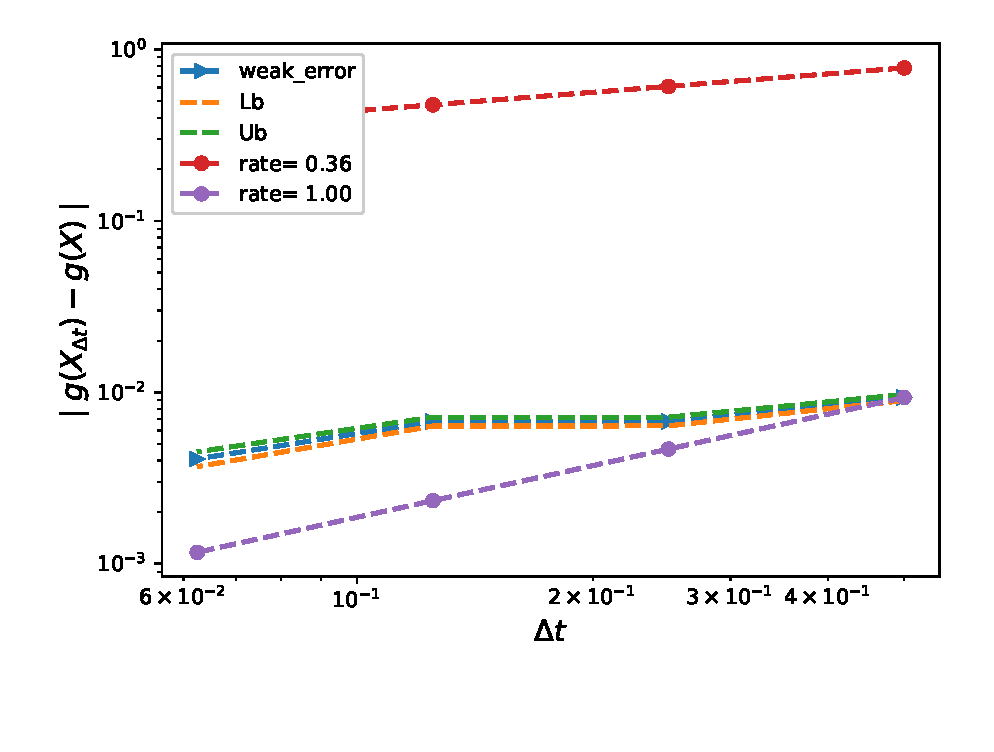
\includegraphics[width=1\linewidth]{./figures/weak_error_rates_basket_3d/without_richardson/weak_convergence_order_basket_option_3d_1_relative_M_7_10_7_plain_1}
%%		\caption{}
%%		\label{fig:sub3}
%%	\end{subfigure}%
%%	\begin{subfigure}{.35\textwidth}
%%		\centering
%%		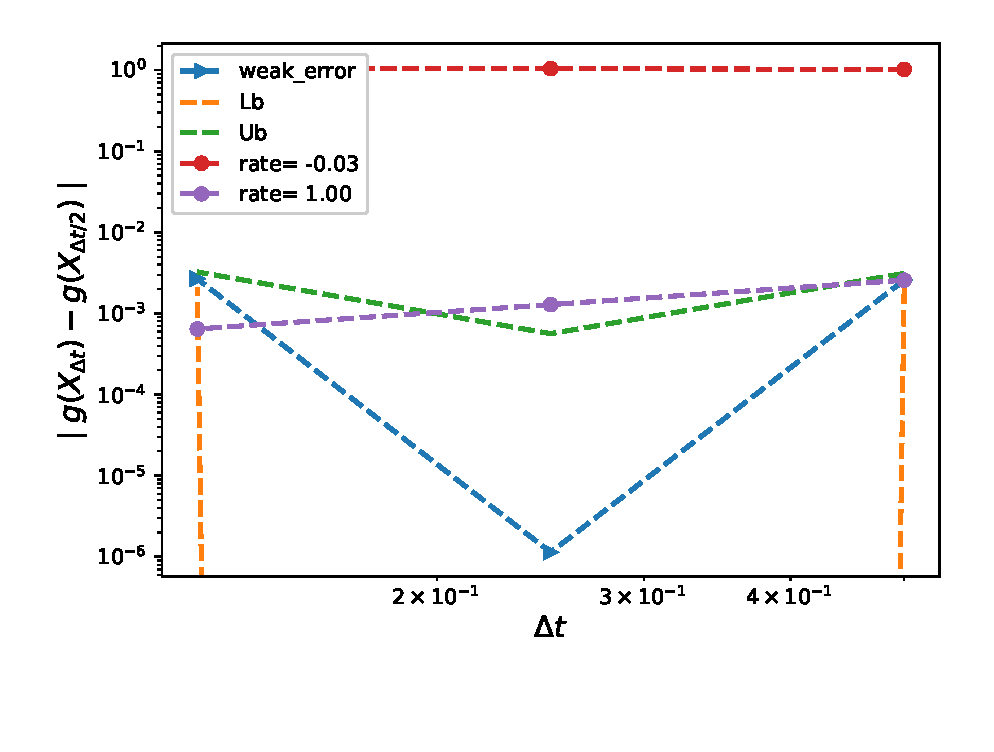
\includegraphics[width=1\linewidth]{./figures/weak_error_rates_basket_3d/without_richardson/weak_convergence_order_differences_basket_option_3d_1_relative_M_7_10_7_plain_1}
%%		\caption{}
%%		\label{fig:sub4}
%%	\end{subfigure}
%%	
%%	\caption{The rate of convergence of the weak error for the Basket ($3$-dimensional) call option, without Richardson extraploation, using MC with $M=7.10^7$: a) $\abs{\expt{g(X_{\Delta t})}-g(X)}$  b) $\abs{\expt{g(X_{\Delta t})-g(X_{\Delta t/2})}}$ }
%%	\label{fig:Weak_rate_basket_3d_without_rich}
%%\end{figure}
%%\FloatBarrier
%%
%%\subsubsection*{Comparing relative errors}\label{sec:Comparing relative errors, basket_3d call}
%%\subsubsection*{Without Richardson extrapolation}
%%
%%
%%\begin{table}[h!]
%%	\centering
%%	\begin{tabular}{l*{6}{c}r}
%%		Method \textbackslash  Steps            & $2$ & $4$ & $8$ & $16$ &   \\
%%		\hline
%%		MISC ($TOl=5.10^{-1},\beta=16$)  & $-$ & $-$ & $-$ & $-$  \\
%%		MISC ($TOl=10^{-1},\beta=16$)   & $-$ & $-$ & $-$ & $-$  \\
%%		MISC ($TOl=5.10^{-2},\beta=16$) & $-$ & $-$ & $-$ & $-$  \\
%%		MISC ($TOl=10^{-2},\beta=16$) & $-$ & $-$ & $-$ & $-$  \\
%%		MISC ($TOl=10^{-3},\beta=16$)  & $-$ & $-$ & $-$ & $-$  \\
%%		MISC ($TOl=10^{-4},\beta=16$)  & $-$ & $-$ & $-$ & $-$  \\
%%		MISC ($TOl=10^{-5},\beta=16$)  & $-$ & $-$ & $-$ & $-$  \\
%%		\hline
%%		MC method ($M=7.10^{7}$)    & $-$ & $-$ & $-$ & $-$  \\
%%		\hline
%%	\end{tabular}
%%	\caption{Basket ($3$-dimensional) Call option price of the different methods for different number of time steps, without Richardson extrapolation.}
%%	\label{table:Basket 3d option price of the different methods for different number of time steps, without Richardson extrapolation, beta_}
%%\end{table}
%%
%%
%%
%%
%%
%%
%%\begin{table}[h!]
%%	\centering
%%	\begin{tabular}{l*{6}{c}r}
%%		Method \textbackslash  Steps            & $2$ & $4$ & $8$ & $16$ &   \\
%%		\hline
%%		MISC ($TOl=5.10^{-1}$)  & $-$ & $-$ & $-$ & $-$  \\
%%		MISC ($TOl=10^{-1}$)   & $-$ & $-$ & $-$ & $-$  \\
%%		MISC ($TOl=5.10^{-2}$)   & $-$ & $-$ & $-$ & $-$  \\
%%		MISC ($TOl=10^{-2}$) & $-$ & $-$ & $-$ & $-$  \\
%%		MISC ($TOl=10^{-3}$)   & $-$ & $-$ & $-$ & $-$  \\
%%		MISC ($TOl=10^{-4}$)   & $-$ & $-$ & $-$ & $-$  \\
%%		MISC ($TOl=10^{-5}$)   & $-$ & $-$ & $-$ & $-$  \\
%%		\hline
%%		MC method +root finding   & $-$ & $-$ & $-$ & $-$  \\
%%		MC method  & $-$ & $-$ & $-$ & $-$  \\
%%		\hline
%%		
%%		Ratio of	$\text{(MC+root finding)}/\text{(MISC)}$  & $-$ & $-$ & $-$ & $-$  \\
%%		Ratio of	$(\text{MC})/(\text{MISC})$ & $-$ & $-$ & $-$ & $-$  \\
%%		\hline
%%	\end{tabular}
%%	\caption{Comparison of the computational time of  MC and MISC, used to compute Basket ($3$-dimensional) Call option price  for different number of time steps, without Richardson extrapolation}
%%	\label{Comparsion of the computational time of  MC and MISC, used to compute Basket 3d Call option price  for different number of time steps, without Richardson extrapolation, beta_16}
%%\end{table}
%

\subsection{The basket option with the smoothing trick as in \cite{bayersmoothing}}\label{sec:The basket option with smoothing trick without a time stepping procedure}

The third experiment that we consider is the pricing of  a European  basket call option in a Black-Scholes model. The basket is composed of $d$ assets ($d=3,8,25$) and we use the same trick of smoothing the integrand that was proposed in \cite{bayersmoothing}. In this case, the dimension of the parameter space $N=d-1$. The interpolation over the parameter space is based on the tensorized Lagrangian interpolation technique with Gaussian  points. The aim of this section is to check the performance of MISC without time stepping. The main goal is to extend this case to the time stepping framework in the next section \ref{sec:The basket option under time stepping framework}


%\newpage
\subsubsection{Results using MISC}
In table \ref{table: Complexity rates of the different experiemnts  for the basket option using BS model}, we summarize the observed  complexity rates for different tested settings for the basket example. From this table, we can check that even with the $25$ dimensional case, the complexity rate in terms of the elapsed time is at least order $1$, which is better than MC, which is $2$. Detailed plots for each case are given by figures (\ref{fig:misc_3D_Basket_1}, \ref{fig:misc_3D_Basket_2}) for $d=3$, figures (\ref{fig:misc_8D_Basket_1}, \ref{fig:misc_8D_Basket_2}) for $d=8$ and figures (\ref{fig:misc_25D_Basket_1}, \ref{fig:misc_25D_Basket_2}) for $d=25$. Mainly, from the plots, 
we checked  that we achive the prescribed tolerance using MISC, the convergence rates of mixed differences which is a basic assumption for using MISC (we observe exponential decay of error rates wrt to the number of quadrature points) and finally the complexity rates. In the next Section, we try to extend these results to the time stepping framework.


\begin{table}[h!]
	\centering
	\begin{tabular}{l*{3}{c}r}
		\# assets  \textbackslash          & $3$ & $8$ & $25$   \\
		\hline
		rate   & $-1/3$ & $-9/20$ & $-16/25$  \\
		\hline
	\end{tabular}
	\caption{Complexity rates of the different experiments  for the basket option using BS model}
	\label{table: Complexity rates of the different experiemnts  for the basket option using BS model}
\end{table}	

\subsubsection*{Case of $3$-dimensional Basket}
\begin{figure}[!h]
	\centering
	\begin{subfigure}{.4\textwidth}
		\centering
		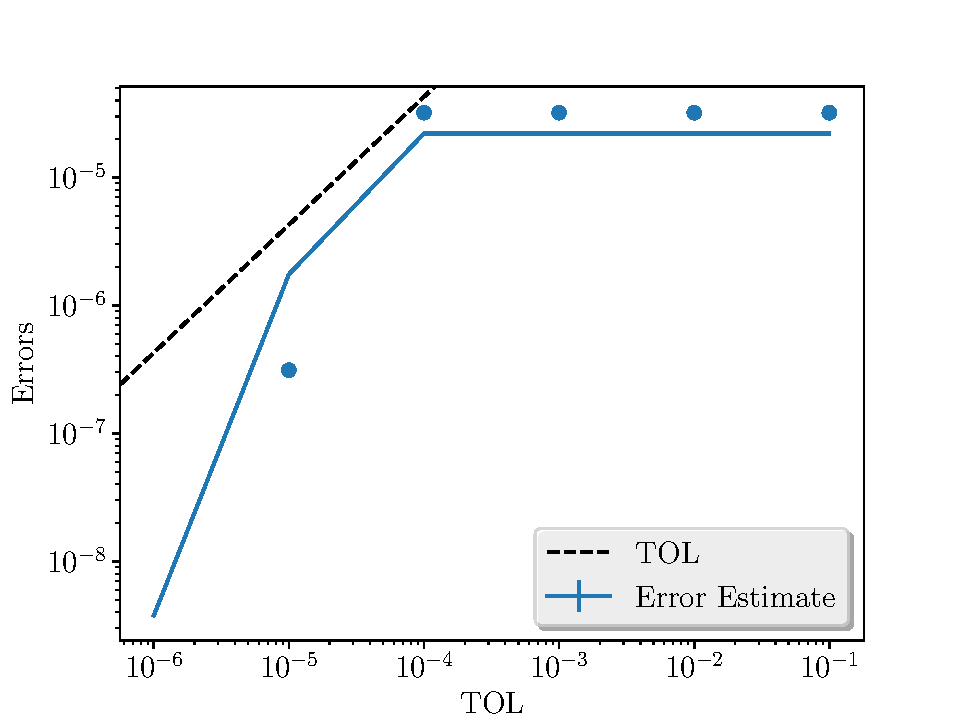
\includegraphics[width=1\linewidth]{./figures/3D_basket/error_estimate.pdf}
		\caption{Error estimate}
		\label{fig:misc_3D_Basket_sub1}
	\end{subfigure}%
	\begin{subfigure}{.4\textwidth}
		\centering
		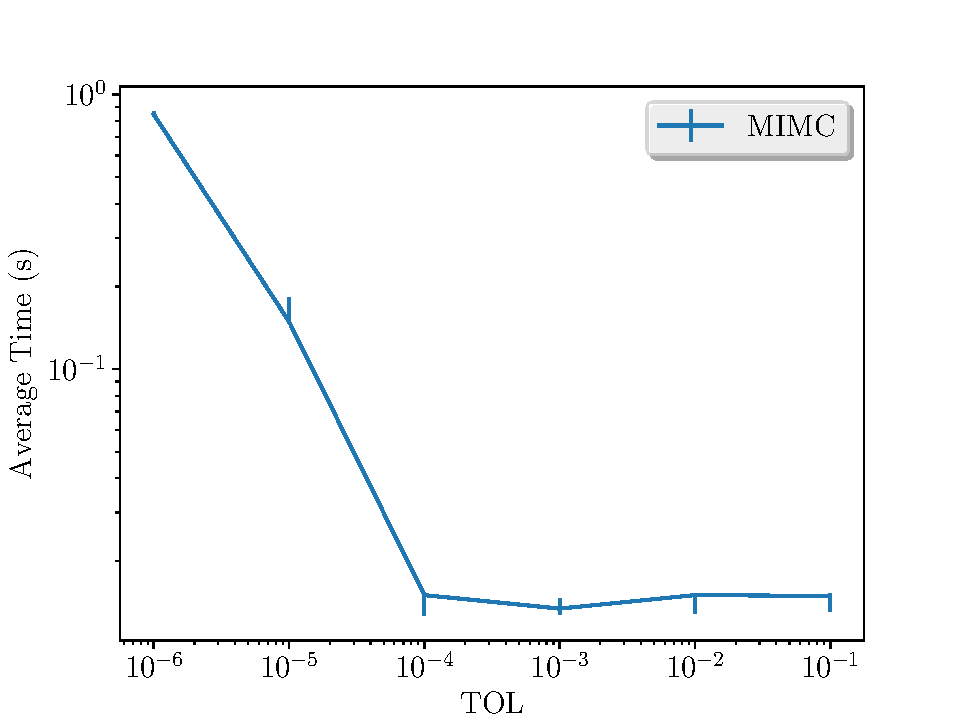
\includegraphics[width=1\linewidth]{./figures/3D_basket/average_running_time.pdf}
		\caption{Average running time as a function of $\text{TOL}$}
		\label{fig:misc_3D_Basket_sub2}
	\end{subfigure}%
	\caption{Convergence and complexity results for the $3$-dimensional basket option using BS model.}
	\label{fig:misc_3D_Basket_1}
\end{figure}



\begin{figure}[!h]
	\centering
	\begin{subfigure}{.4\textwidth}
		\centering
		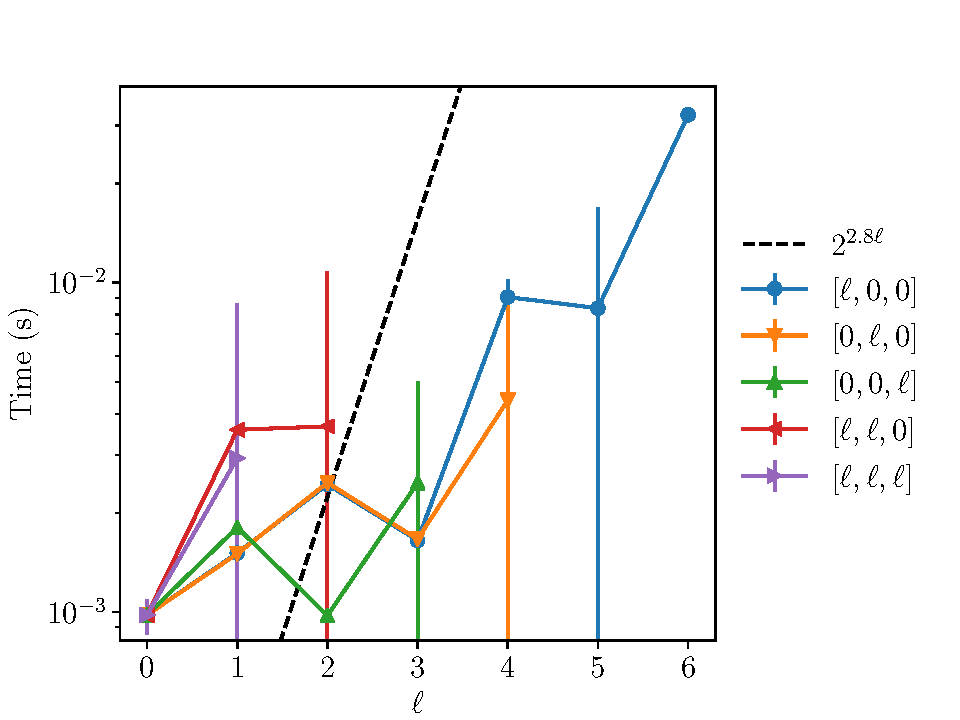
\includegraphics[width=1\linewidth]{./figures/3D_basket/level_work.pdf}
		\caption{Average Computational time per level.}
		\label{fig:misc_3D_Basket_sub3}
	\end{subfigure}%
	\begin{subfigure}{.4\textwidth}
		\centering
		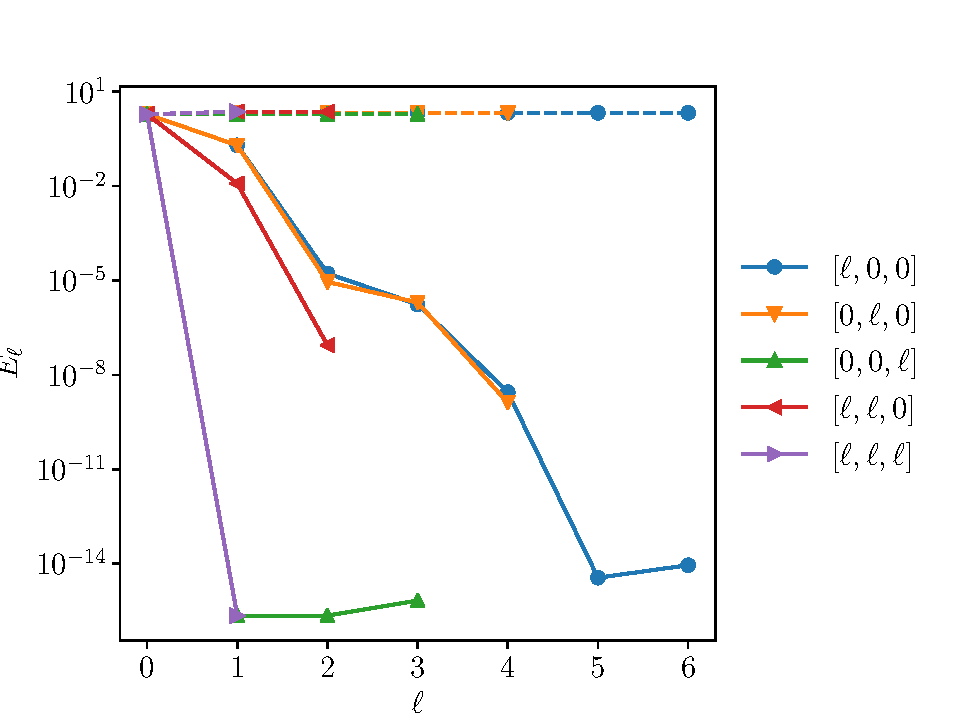
\includegraphics[width=1\linewidth]{./figures/3D_basket/levels_error_rate.pdf}
		\caption{The convergence rate of mixed differences per level.}
		\label{fig:misc_3D_Basket_sub4}
	\end{subfigure}%
	\caption{Convergence and work rates for discretization levels for the $3$-dimensional basket option using BS model.}
	\label{fig:misc_3D_Basket_2}
\end{figure}

\FloatBarrier


\subsubsection*{Case of $8$-dimensional Basket}
\begin{figure}[!h]
	\centering
	\begin{subfigure}{.4\textwidth}
		\centering
		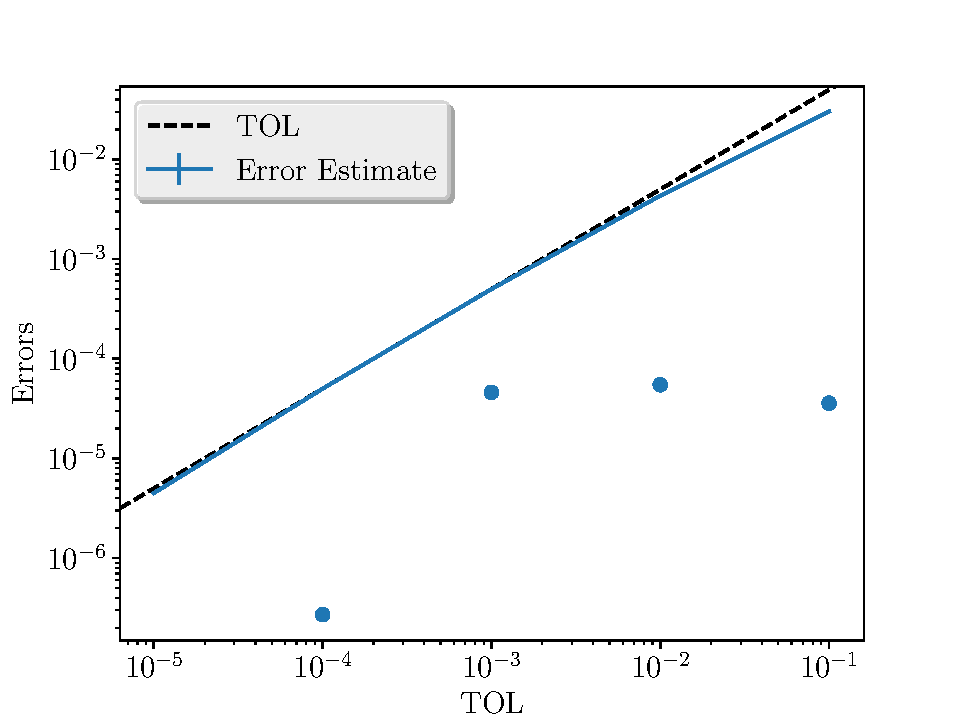
\includegraphics[width=1\linewidth]{./figures/8D_basket/error_estimate.pdf}
		\caption{Error estimate}
		\label{fig:misc_8D_Basket_sub1}
	\end{subfigure}%
	\begin{subfigure}{.4\textwidth}
		\centering
		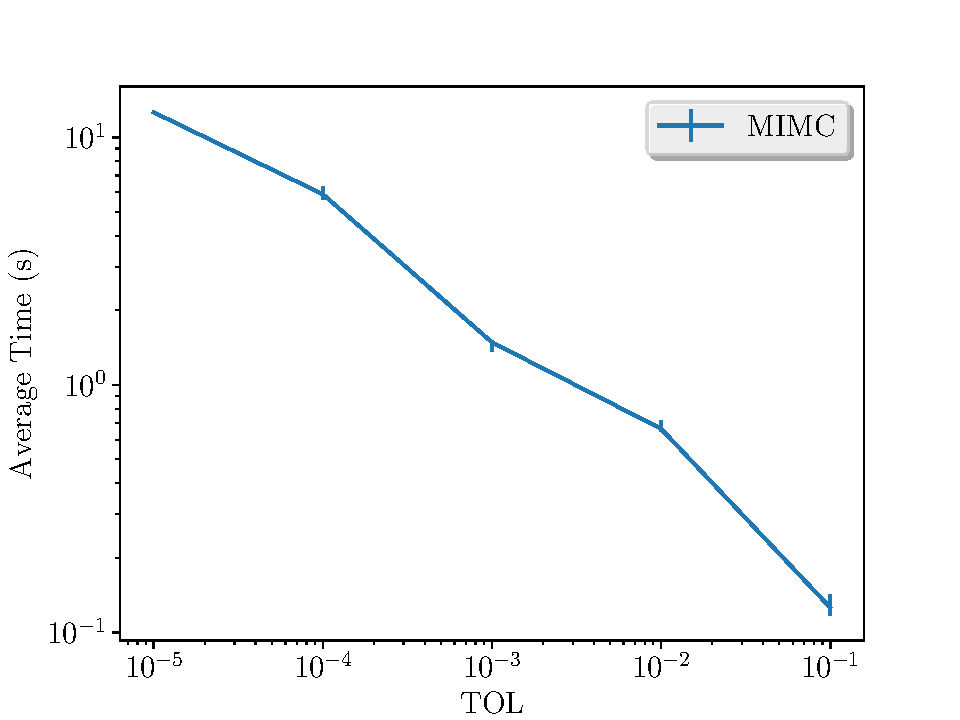
\includegraphics[width=1\linewidth]{./figures/8D_basket/average_running_time.pdf}
		\caption{Average running time as a function of $TOL$}
		\label{fig:misc_8D_Basket_sub2}
	\end{subfigure}%
	\caption{Convergence and complexity results for  the $8$-dimensional basket option using BS model.}
	\label{fig:misc_8D_Basket_1}
\end{figure}



\begin{figure}[!h]
	\centering
	\begin{subfigure}{.4\textwidth}
		\centering
		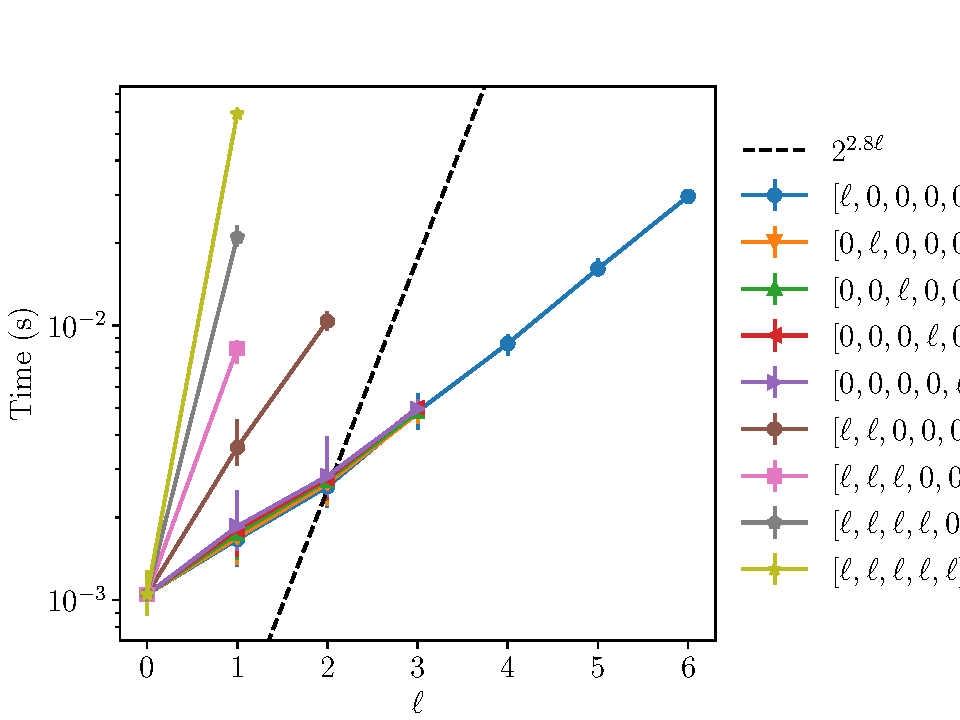
\includegraphics[width=1\linewidth]{./figures/8D_basket/level_work.pdf}
		\caption{Average Computational time per level.}
		\label{fig:misc_8D_Basket_sub3}
	\end{subfigure}%
	\begin{subfigure}{.4\textwidth}
		\centering
		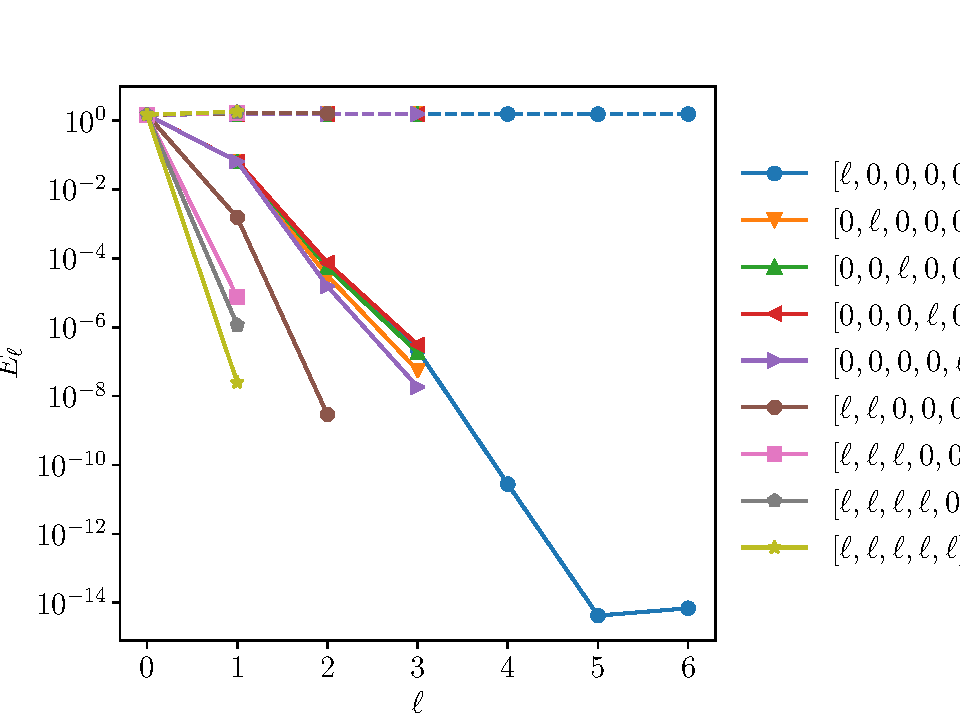
\includegraphics[width=1\linewidth]{./figures/8D_basket/levels_error_rate.pdf}
		\caption{The convergence rate of mixed differences per level.}
		\label{fig:misc_8D_Basket_sub4}
	\end{subfigure}%
	\caption{Convergence and work rates for discretization levels for the $8$-dimensional basket option using BS model.}
	\label{fig:misc_8D_Basket_2}
\end{figure}
\FloatBarrier

\subsubsection*{Case of $25$-dimensional Basket}
\begin{figure}[h!]
	\centering
	\begin{subfigure}{.4\textwidth}
		\centering
		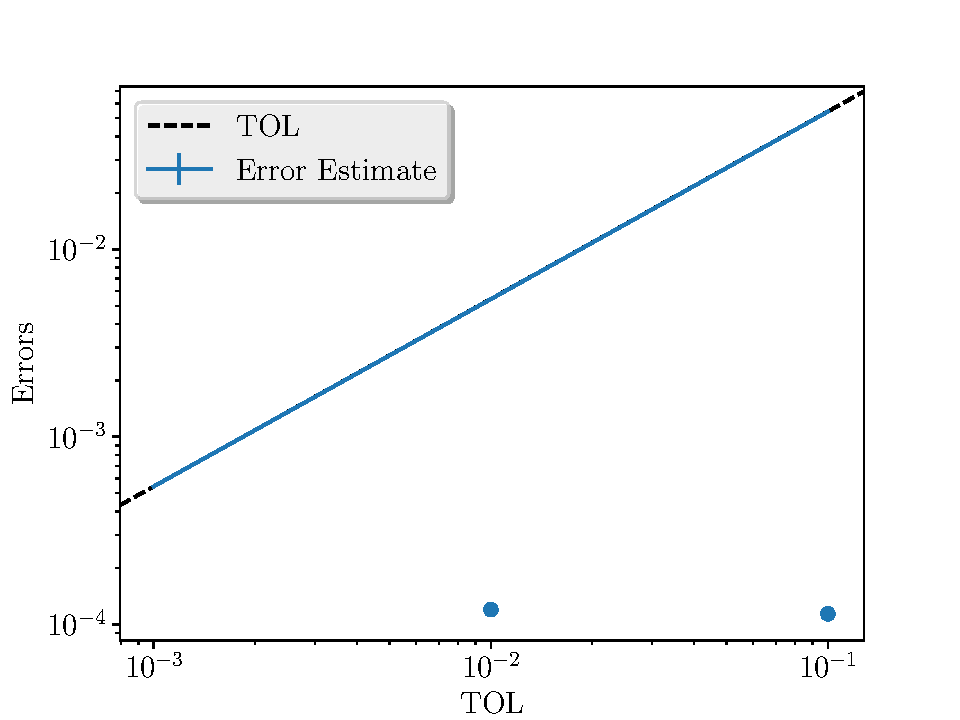
\includegraphics[width=1\linewidth]{./figures/25D_basket/error_estimate.pdf}
		\caption{Error estimate}
		\label{fig:misc_25D_Basket_sub1}
	\end{subfigure}%
	\begin{subfigure}{.4\textwidth}
		\centering
		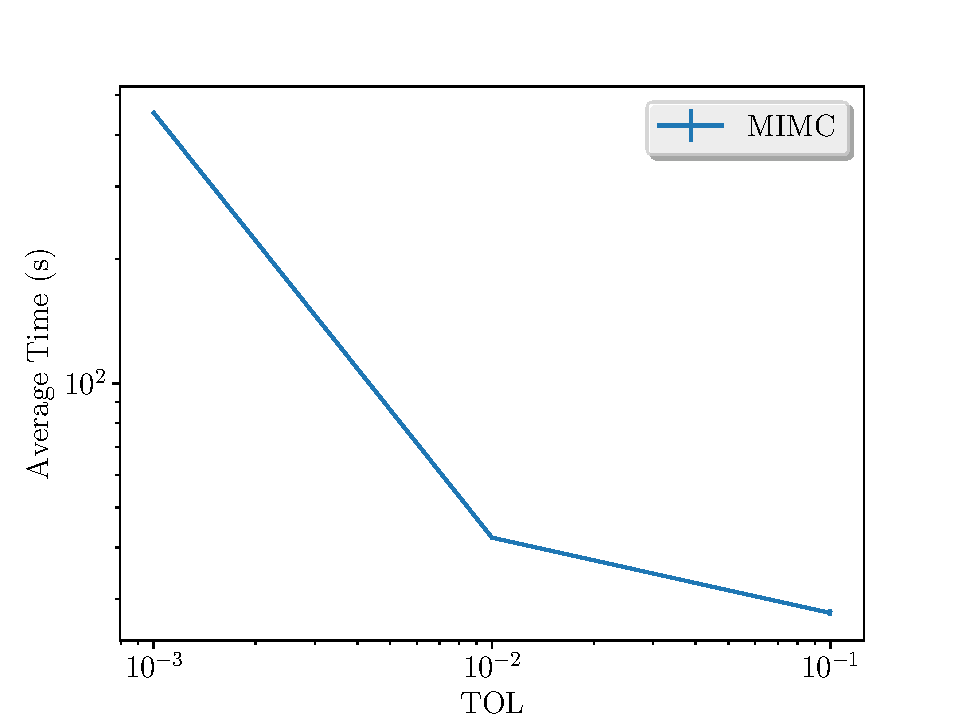
\includegraphics[width=1\linewidth]{./figures/25D_basket/average_running_time.pdf}
		\caption{Average running time as a function of $TOL$}
		\label{fig:misc_25D_Basket_sub2}
	\end{subfigure}%
	\caption{Convergence and complexity results for  the $25$-dimensional basket option using BS model.}
	\label{fig:misc_25D_Basket_1}
\end{figure}



\begin{figure}[h!]
	\centering
	\begin{subfigure}{.4\textwidth}
		\centering
		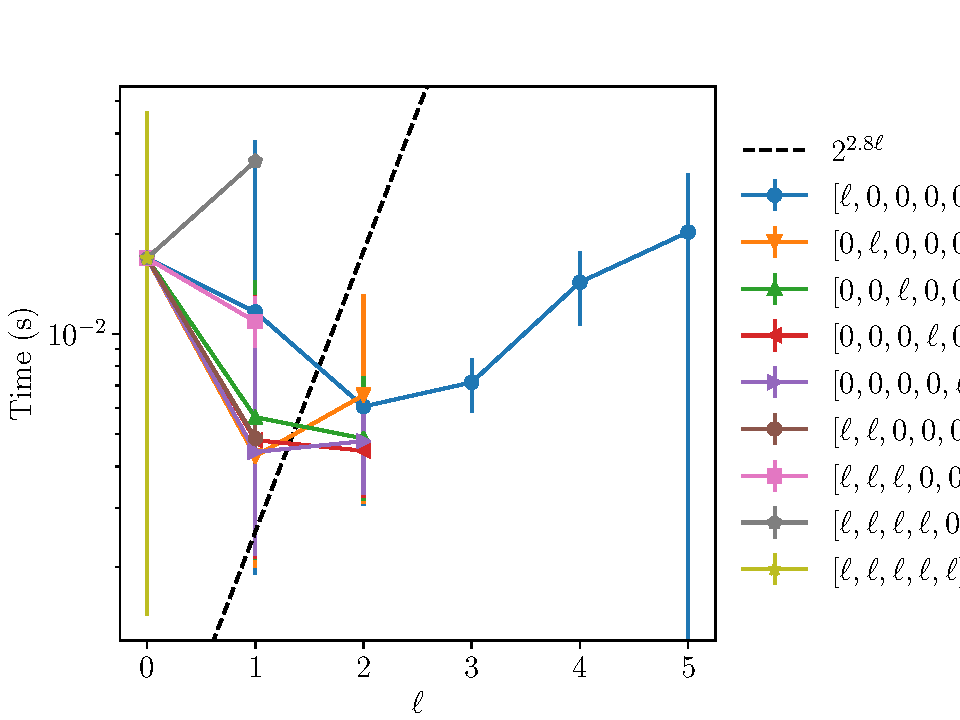
\includegraphics[width=1\linewidth]{./figures/25D_basket/level_work.pdf}
		\caption{Average Computational time per level.}
		\label{fig:misc_25D_Basket_sub3}
	\end{subfigure}%
	\begin{subfigure}{.4\textwidth}
		\centering
		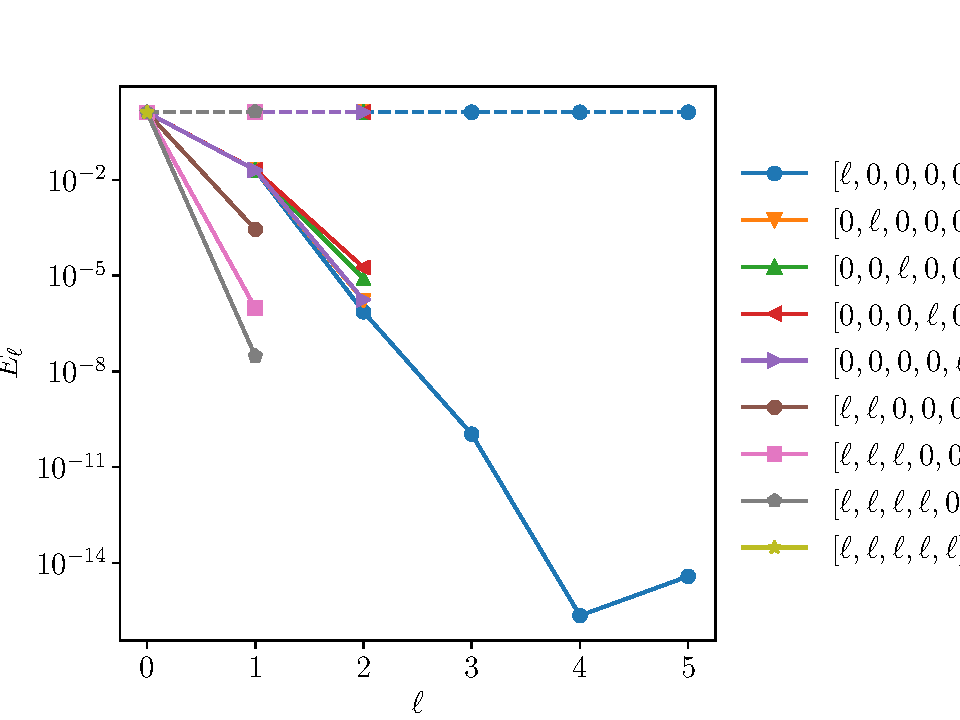
\includegraphics[width=1\linewidth]{./figures/25D_basket/levels_error_rate.pdf}
		\caption{The convergence rate of mixed differences per level.}
		\label{fig:misc_25D_Basket_sub4}
	\end{subfigure}%
	\caption{Convergence and work rates for discretization levels for the $25$-dimensional basket option using BS model.}
	\label{fig:misc_25D_Basket_2}
\end{figure}


\FloatBarrier 




%\subsection{Results for  the CIR process}
%
%The impact of the Brownian bridge will disappear in the limit, which may make the effect of the smoothing, but also of the errors in the kink location difficult to identify . For this reason, we study a more complicated 1-dimensional problem. In fact, we use a CIR process. To avoid complications at the boundary, we use nice parameter choices, such that the discretized process is very unlikely to hit the boundary (Feller condition).
%
%
%
%The CIR model specifies that the instantaneous interest rate follows the SDE given by
%\begin{equation}\label{CIR_process}
%dX_t=a(b-X_t)dt+\sigma \sqrt{X_t} dW_t,\: X(0)=X_0>0
%\end{equation}
%where and $a>0$, $b>0$ and $\sigma>0$, are the parameters. The parameter $a$ corresponds to the speed of adjustment, $b$ to the mean and $\sigma$ to volatility. 
%
%If the parameters obey the following condition (known as the Feller condition) then the process $X_t$  is strictly positive
%\begin{equation}\label{Feller_condition}
%2 a b \geq\sigma^2.
%\end{equation}
%
%The SDE \eqref{CIR_process} is not explicitly solvable. In general there are two ways to do it, namely, exact simulation methods and approximation schemes. Exact simulation in general requires more time
%than a simulation with approximation schemes (Up to a factor 10). Therefore, it is used to compute expectations that depend on the values of the process at just a few fixed times. However, for expectations that depends on all the path (such as integrals) discretization schemes should be preferred. 
%
%The main problem  when discretizing a CIR process using Euler scheme is that it can lead to negative values for which the square root is not defined. In fact, if we consider the following straightforward Euler scheme on the time interval $[0,T]$ for a CIR process $X(t)$:
%\begin{equation}\label{Euler_CIR}
%\bar{X}(t_{i+1})=\bar{X}(t_i)+a(b-\bar{X}(t_i)) \Delta t_i+\sigma \sqrt{\bar{X}(t_i)} \Delta W_i,
%\end{equation}
%
%then it can lead to negative values since the Gaussian
%increment is not bounded from below. Thus, this  scheme is not well defined.
%
%Many modified Euler schemes were proposed to overcome this issue. For instance, Deelstra and Delbaen \cite{deelstra1998convergence} have propose the full truncation scheme given by
%\begin{equation}\label{Full_truncation_CIR}
%\bar{X}(t_{i+1})=\bar{X}(t_i)+a(b-\bar{X}(t_i)) \Delta t_i+\sigma \sqrt{\bar{X}(t_i)^+} \Delta W_i.
%\end{equation}
%
%Higham and Mao \cite{mao2007stochastic} proposed the following scheme
% \begin{equation}\label{partial_reflection_CIR}
% \bar{X}(t_{i+1})=\bar{X}(t_i)+a(b-\bar{X}(t_i)) \Delta t_i+\sigma \sqrt{\abs{\bar{X}(t_i)}} \Delta W_i.
% \end{equation}
% Lord et al \cite{lord2010comparison} proposed the following scheme
% 
% \begin{equation}\label{truncation_CIR}
% \bar{X}(t_{i+1})=\bar{X}(t_i)+a(b-\bar{X}(t_i)^+) \Delta t_i+\sigma \sqrt{\bar{X}(t_i)^+} \Delta W_i.
% \end{equation}
% 
% 
%Diop proposed in \cite{berkaoui2008euler} proposed the reflection scheme, given by
%\begin{equation}\label{Reflection_CIR}
%\bar{X}(t_{i+1})=\mid\bar{X}(t_i)+a(b-\bar{X}(t_i)) \Delta t_i+\sigma \sqrt{\bar{X}(t_i)} \Delta W_i \mid.
%\end{equation}
%Also, implicit and higher order schemes were proposed by Alfonsi \cite{alfonsi2005discretization,alfonsi2008second,alfonsi2010high}.
%
%Those modified Euler schemes were studied  numerically in \cite{alfonsi2005discretization}. It is observed that when $\sigma$ is small enough, typically $\sigma^2 \le 2a$, these schemes have a weak error of order one and a strong error of order $1/2$. However, when $\sigma$ is getting large, say $\sigma^2\gg 4a$, the convergence of all these schemes is degraded. As observed
%by Lord et al. \cite{lord2010comparison}, the schemes \eqref{Full_truncation_CIR} and \eqref{truncation_CIR} behave better than the schemes \eqref{partial_reflection_CIR} and \eqref{Reflection_CIR}. In fact, when $\sigma$ gets large, the CIR process spends more time close to zero and get stuck in the neighbourhood of zero when $\sigma$ is really large. When the scheme takes a negative value, the absolute value in  both schemes (\eqref{partial_reflection_CIR},\eqref{Reflection_CIR}) produces a noise that pushes the scheme away from zero. On the other hand, the positive part in truncation schemes cancels the noise when the scheme gets negative, which better reproduces the behaviour of the
%CIR process. 
%
%In the following, we use the scheme given by \eqref{Full_truncation_CIR} to simulate the discrete CIR process.
%\subsubsection{Location of the kink for the discrete problem: Using full truncation scheme}\label{sec:kink_location_full_truncation)_CIR}
%
%
%The full truncation scheme simulating the CIR process is given by \eqref{Full_truncation_CIR}. Here we are interested in finding the location of the kink for hockey-stick function.
%
%
%Using Brownian bridge construction given by \eqref{Brownian_bridge}, we have
%\begin{align}\label{recursion_full_truncation_CIR}
%X_{t_1}&= X_{t_0} \left[ 1- a \Delta t  \right]+ \sigma \sqrt{X_{t_0}^+} \left[   Y \frac{\Delta t}{\sqrt{T}} + \Delta B_0\right]+ ab \Delta t\nonumber\\
%X_{t_2}&= X_{t_1} \left[ 1- a \Delta t  \right]+ \sigma \sqrt{X_{t_1}^+} \left[   Y \frac{\Delta t}{\sqrt{T}} + \Delta B_1\right]+ ab \Delta t \nonumber\\ 
%\vdots &= \vdots =\vdots \nonumber\\
%X_{t_N}&= X_{t_{N-1}} \left[ 1- a \Delta t  \right]+ \sigma \sqrt{X_{t_{N-1}}^+} \left[   Y \frac{\Delta t}{\sqrt{T}} + \Delta B_{N-1} \right]+ ab \Delta t ,
%\end{align}
%
%
%to simplify the notation we set $f_i(y):=X_{t_i}$. Then  the location of the kink point for the approximate problem is equivalent to finding the roots of the polynomial $P(y_\ast(K))$, given by
%\begin{align}\label{polynomial_kink_location_CIR_full_truncation}
%P(y_{\ast}(K))=f_N(y_\ast(K))-\frac{K}{X_0},
%\end{align}
%where $f_N(y)$ is computed using recursion \eqref{recursion_full_truncation_CIR}.
%
%To apply the \textbf{Newton iteration method}, we need the derivative $P'=\frac{d P}{d y_\ast}=f_N'$, which is deduced from recursion \eqref{recursion_full_truncation_CIR}, and given by the the following relation
%\begin{align}
%f_i'(y) &= f_{i-1}'(y)\left[1-a \Delta t \right]+ \sigma \sqrt{f_{i-1}(y)^+} \left[ \frac{\Delta t}{\sqrt{T}}+ \left[y \frac{\Delta t}{\sqrt{T}}+\Delta B_{i-1}\right] \frac{f_{i-1}'(y)}{2} \right],\: 1 \le i \le N \nonumber\\
%f_0'&=0.
%\end{align}
%
%
%
%
%\subsubsection{Results}
%The code of this section is found in the script discretized\_CIR.py, which compares the different ways of determining the kink location for 1D CIR model.
%
%
%
%
%
%
%\FloatBarrier

